\newcommand{\econtexRoot}{Paper/}
% The \commands below are required to allow sharing of the same base code via Github between TeXLive on a local machine and ShareLaTeX.  This is an ugly solution to the requirement that custom LaTeX packages be accessible, and that ShareLaTeX seems to ignore symbolic links (even if they are relative links to valid locations)
\providecommand{\econtex}{\econtexRoot/texmf-local/tex/latex/econtex}
\providecommand{\econtexSetup}{\econtexRoot/texmf-local/tex/latex/econtexSetup}
\providecommand{\econtexShortcuts}{\econtexRoot/texmf-local/tex/latex/econtexShortcuts}
\providecommand{\econtexBibMake}{\econtexRoot/texmf-local/tex/latex/econtexBibMake}
\providecommand{\econtexBibStyle}{\econtexRoot/texmf-local/bibtex/bst/econtex}
\providecommand{\notes}{\econtexRoot/texmf-local/tex/latex/handout}
\providecommand{\handoutSetup}{\econtexRoot/texmf-local/tex/latex/handoutSetup}
\providecommand{\handoutShortcuts}{\econtexRoot/texmf-local/tex/latex/handoutShortcuts}
\providecommand{\handoutBibMake}{\econtexRoot/texmf-local/tex/latex/handoutBibMake}
\providecommand{\handoutBibStyle}{\econtexRoot/texmf-local/bibtex/bst/handout}

  

\documentclass{beamer}  %[handout]
\usepackage{remreset}
\usepackage{etoolbox}
\usepackage{comment}
\usepackage{graphicx}
%\usepackage{dtklogos}
\usepackage{dsfont}
\usepackage{amsmath,amssymb}
\usepackage{\econtexShortcuts}
\usepackage[english]{babel}
\usepackage{tikz} 
\usetikzlibrary{tikzmark,fit,shapes.geometric}
\usetikzlibrary{tikzmark,calc,arrows,shapes,decorations.pathreplacing}
\tikzset{every picture/.style={remember picture}}
\usepackage{cancel}
\usepackage{booktabs,natbib}
\setbeamercovered{invisible}

\usepackage{dcolumn}


\makeatletter
\@removefromreset{subsection}{section}
\patchcmd{\beamer@part}{\setcounter{subsection}{0}}{}{}
\makeatother
\setcounter{subsection}{1}
\setbeamercovered{transparent}
\setbeamertemplate{navigation symbols}{}%remove navigation symbols

\mode<presentation>{}
%% preamble
\title[Consumption Heterogeneity: Micro Drivers and Macro Implications]{Consumption Heterogeneity: \\ Micro Drivers and Macro Implications}
\author{Edmund Crawley \& Andreas Kuchler}
\date[9/28/2018]{Norges Bank, Danmarks Nationalbank and Deutsche Bundesbank conference on Heterogeneous households, firms and financial intermediaries
\\
September 28, 2018}
\usetheme{Frankfurt}
\begin{document}
\newcolumntype{d}[1]{D{.}{.}{#1}}
%circled draws a circle around a number
\newcommand*\circled[1]{\tikz[baseline=(char.base)]{
		\node[shape=circle,draw,inner sep=2pt] (char) {#1};}}


\frame{\titlepage}
\section{Motivation}
\setbeamercovered{invisible}
\frame
{
	\frametitle{Is Heterogeneity Important for Macroeconomics?}
\textbf{Theory:} Consumption heterogeneity is \textit{potentially} very important for macroeconomic dynamics
\begin{itemize}
	\item e.g. Recent HANK models\\
\end{itemize}
\bigskip
Macroeconomic events can redistribute wealth between High and Low MPC households, affecting aggregate consumption\\
\bigskip
\pause
\textbf{Empirics:} Testing and quantifying these effects often boils down to measuring the distribution of MPC along some dimension of redistribution\\
\bigskip
Ability to do so is limited by:
\begin{itemize}
	\item Methods to measure MPCs
	\item Consumption data
	\item Household balance sheet data
\end{itemize}	
}
\frame
{
	\frametitle{What does this paper do?}
	Two Empirical Contributions\\
	\begin{itemize}
	\item[1] \textbf{Method:} New methodology to measure MPCs out of transitory and permanent income shocks
	\begin{itemize}
		\item Builds on \cite{blundell_consumption_2008}
		\item Correctly accounts for the Time Aggregation Problem
	\end{itemize}
	\bigskip
	\item[2] \textbf{Data:} Panel data covering all Danish households 2004-2015 
	\begin{itemize}
		\item Large sample size reveals clear, systemic heterogeneity
		\item Detailed household balance sheets allow us to infer implications for monetary policy transmission
	\end{itemize}
	\end{itemize}
	\pause
	\bigskip
	We also test to what extent a buffer-stock model can fit the observed distribution of MPC with liquid wealth
}
\frame
{
	\frametitle{What does this paper find?}
	\begin{tikzpicture}
	\node (img1) {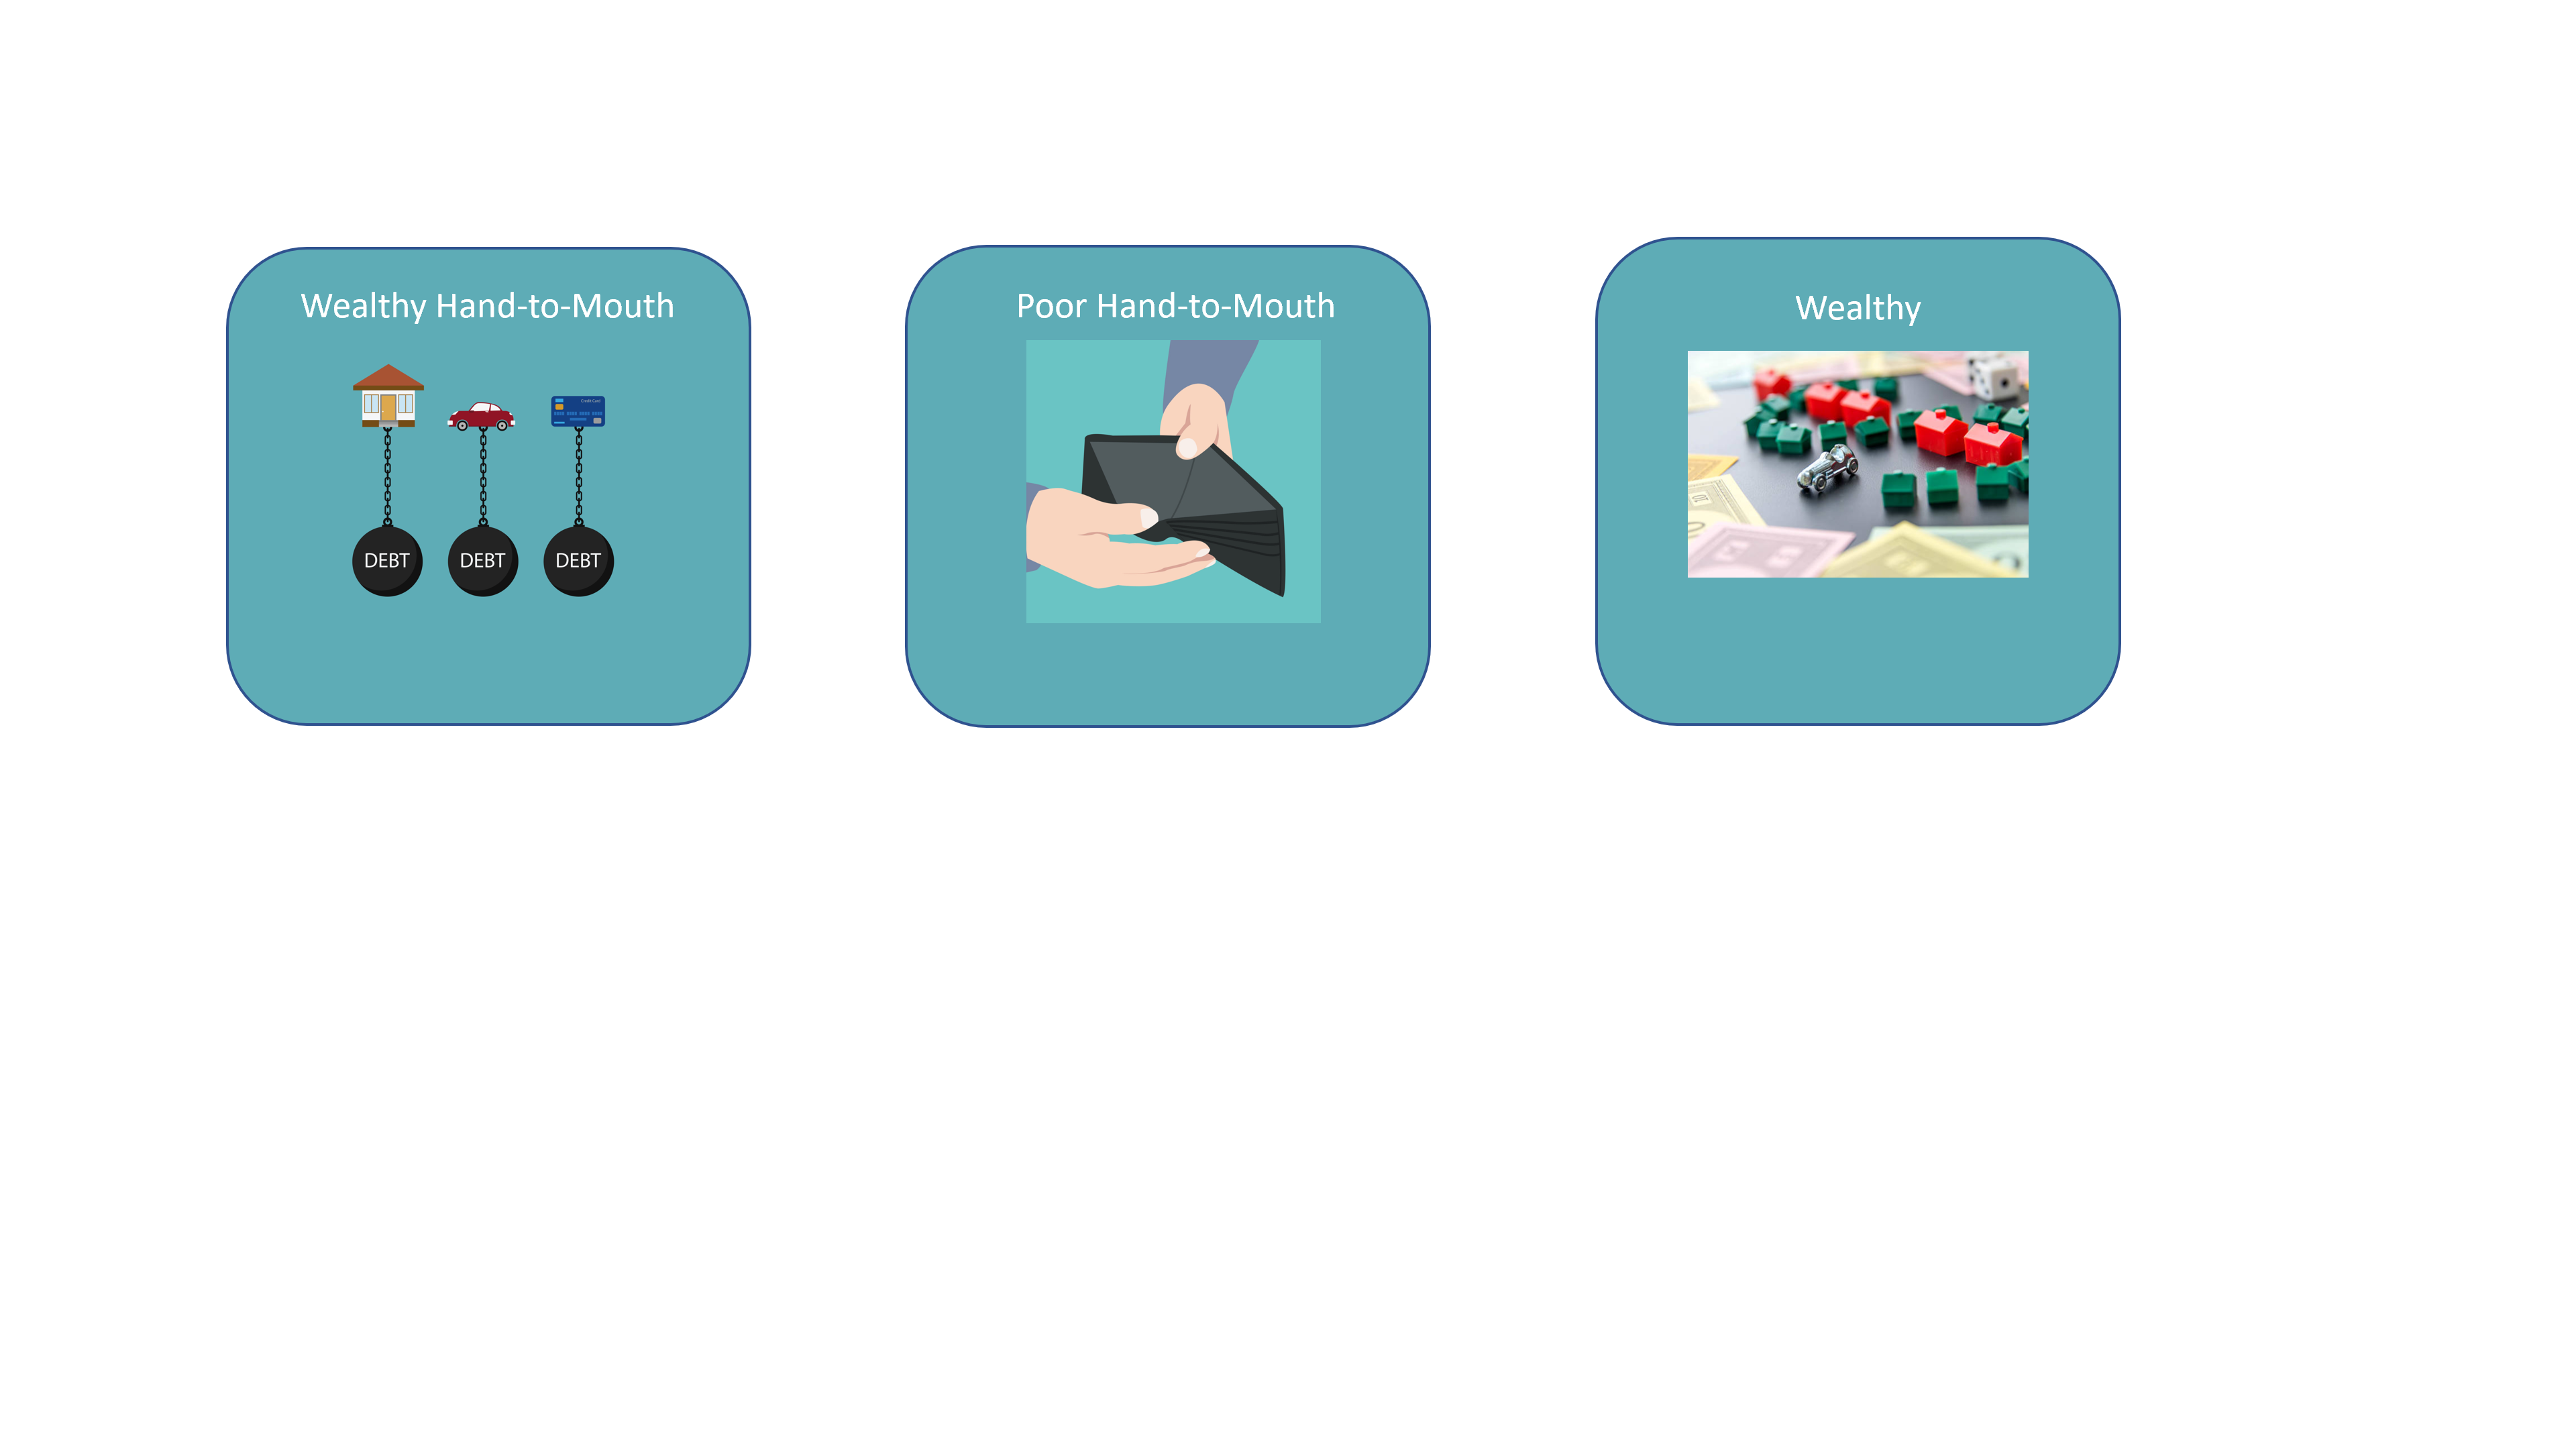
\includegraphics[height=6cm,trim= 3cm 1.9cm 0 3.5cm, clip]{./SlideFigures/IRE1.png}};
	\pause
	\node (img2) {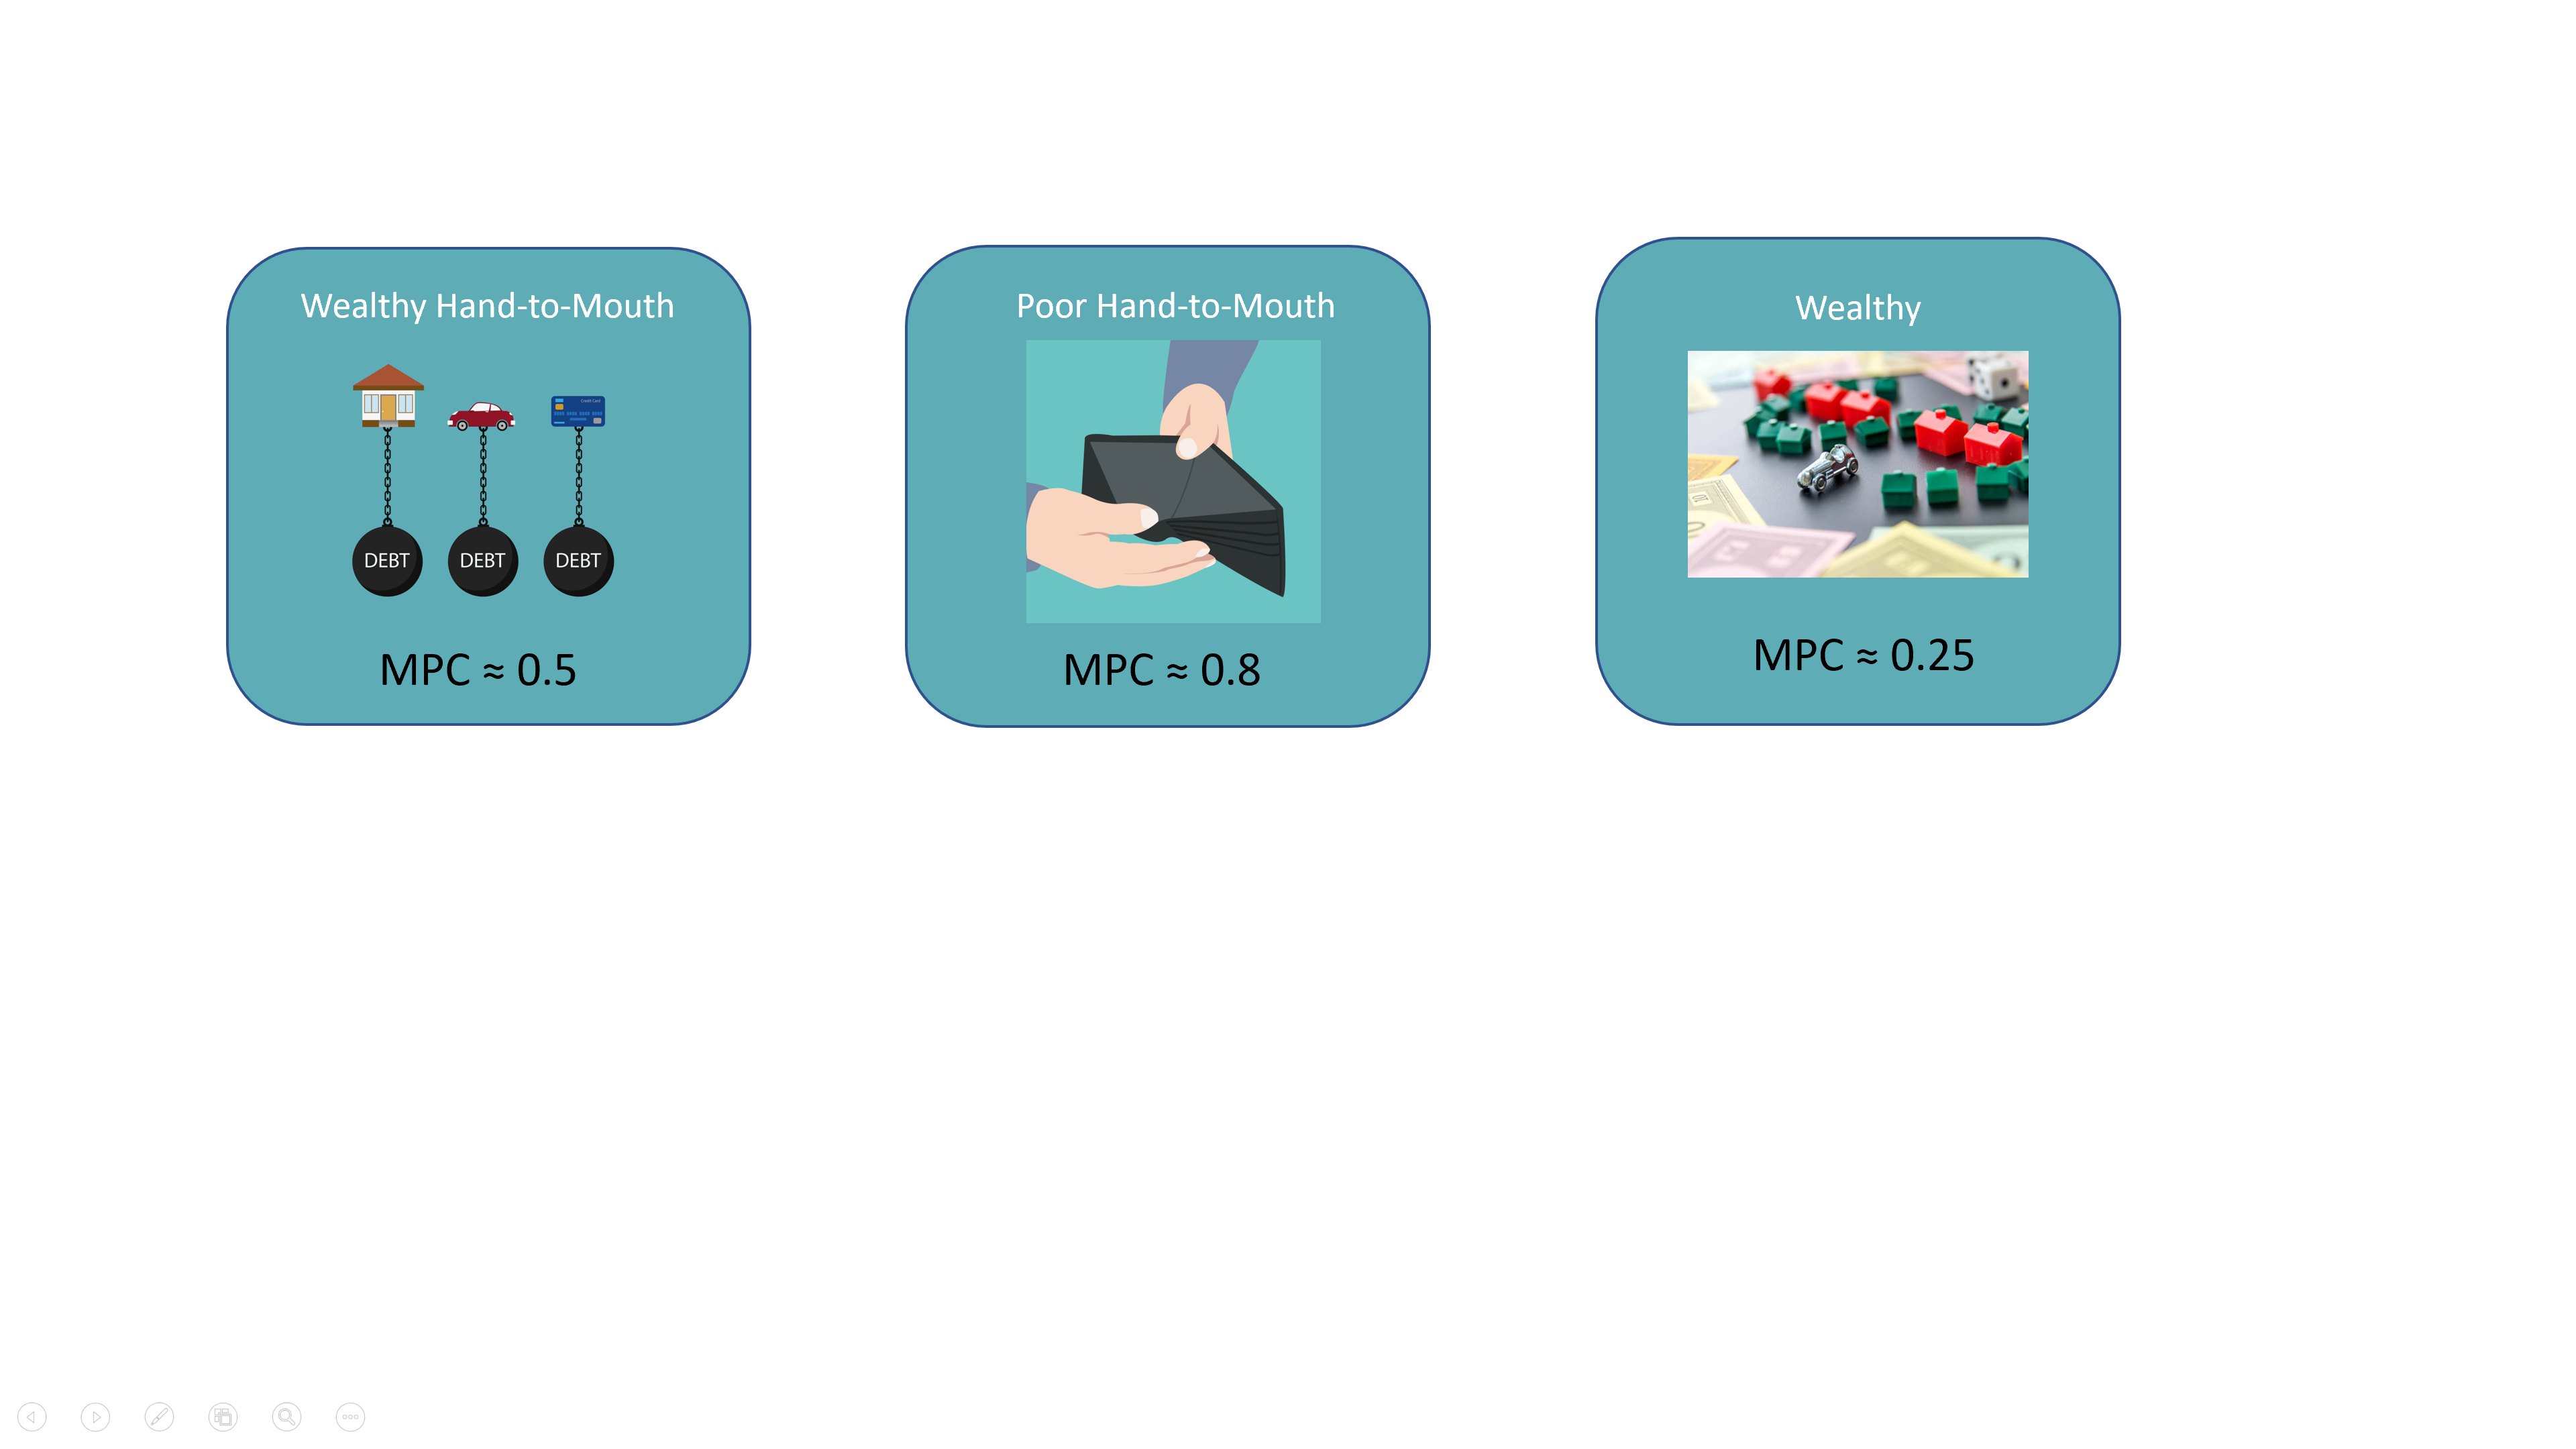
\includegraphics[height=6cm,trim= 3cm 1.9cm 0 3.5cm, clip]{./SlideFigures/IRE2.png}};
	\pause
	\node (img3) {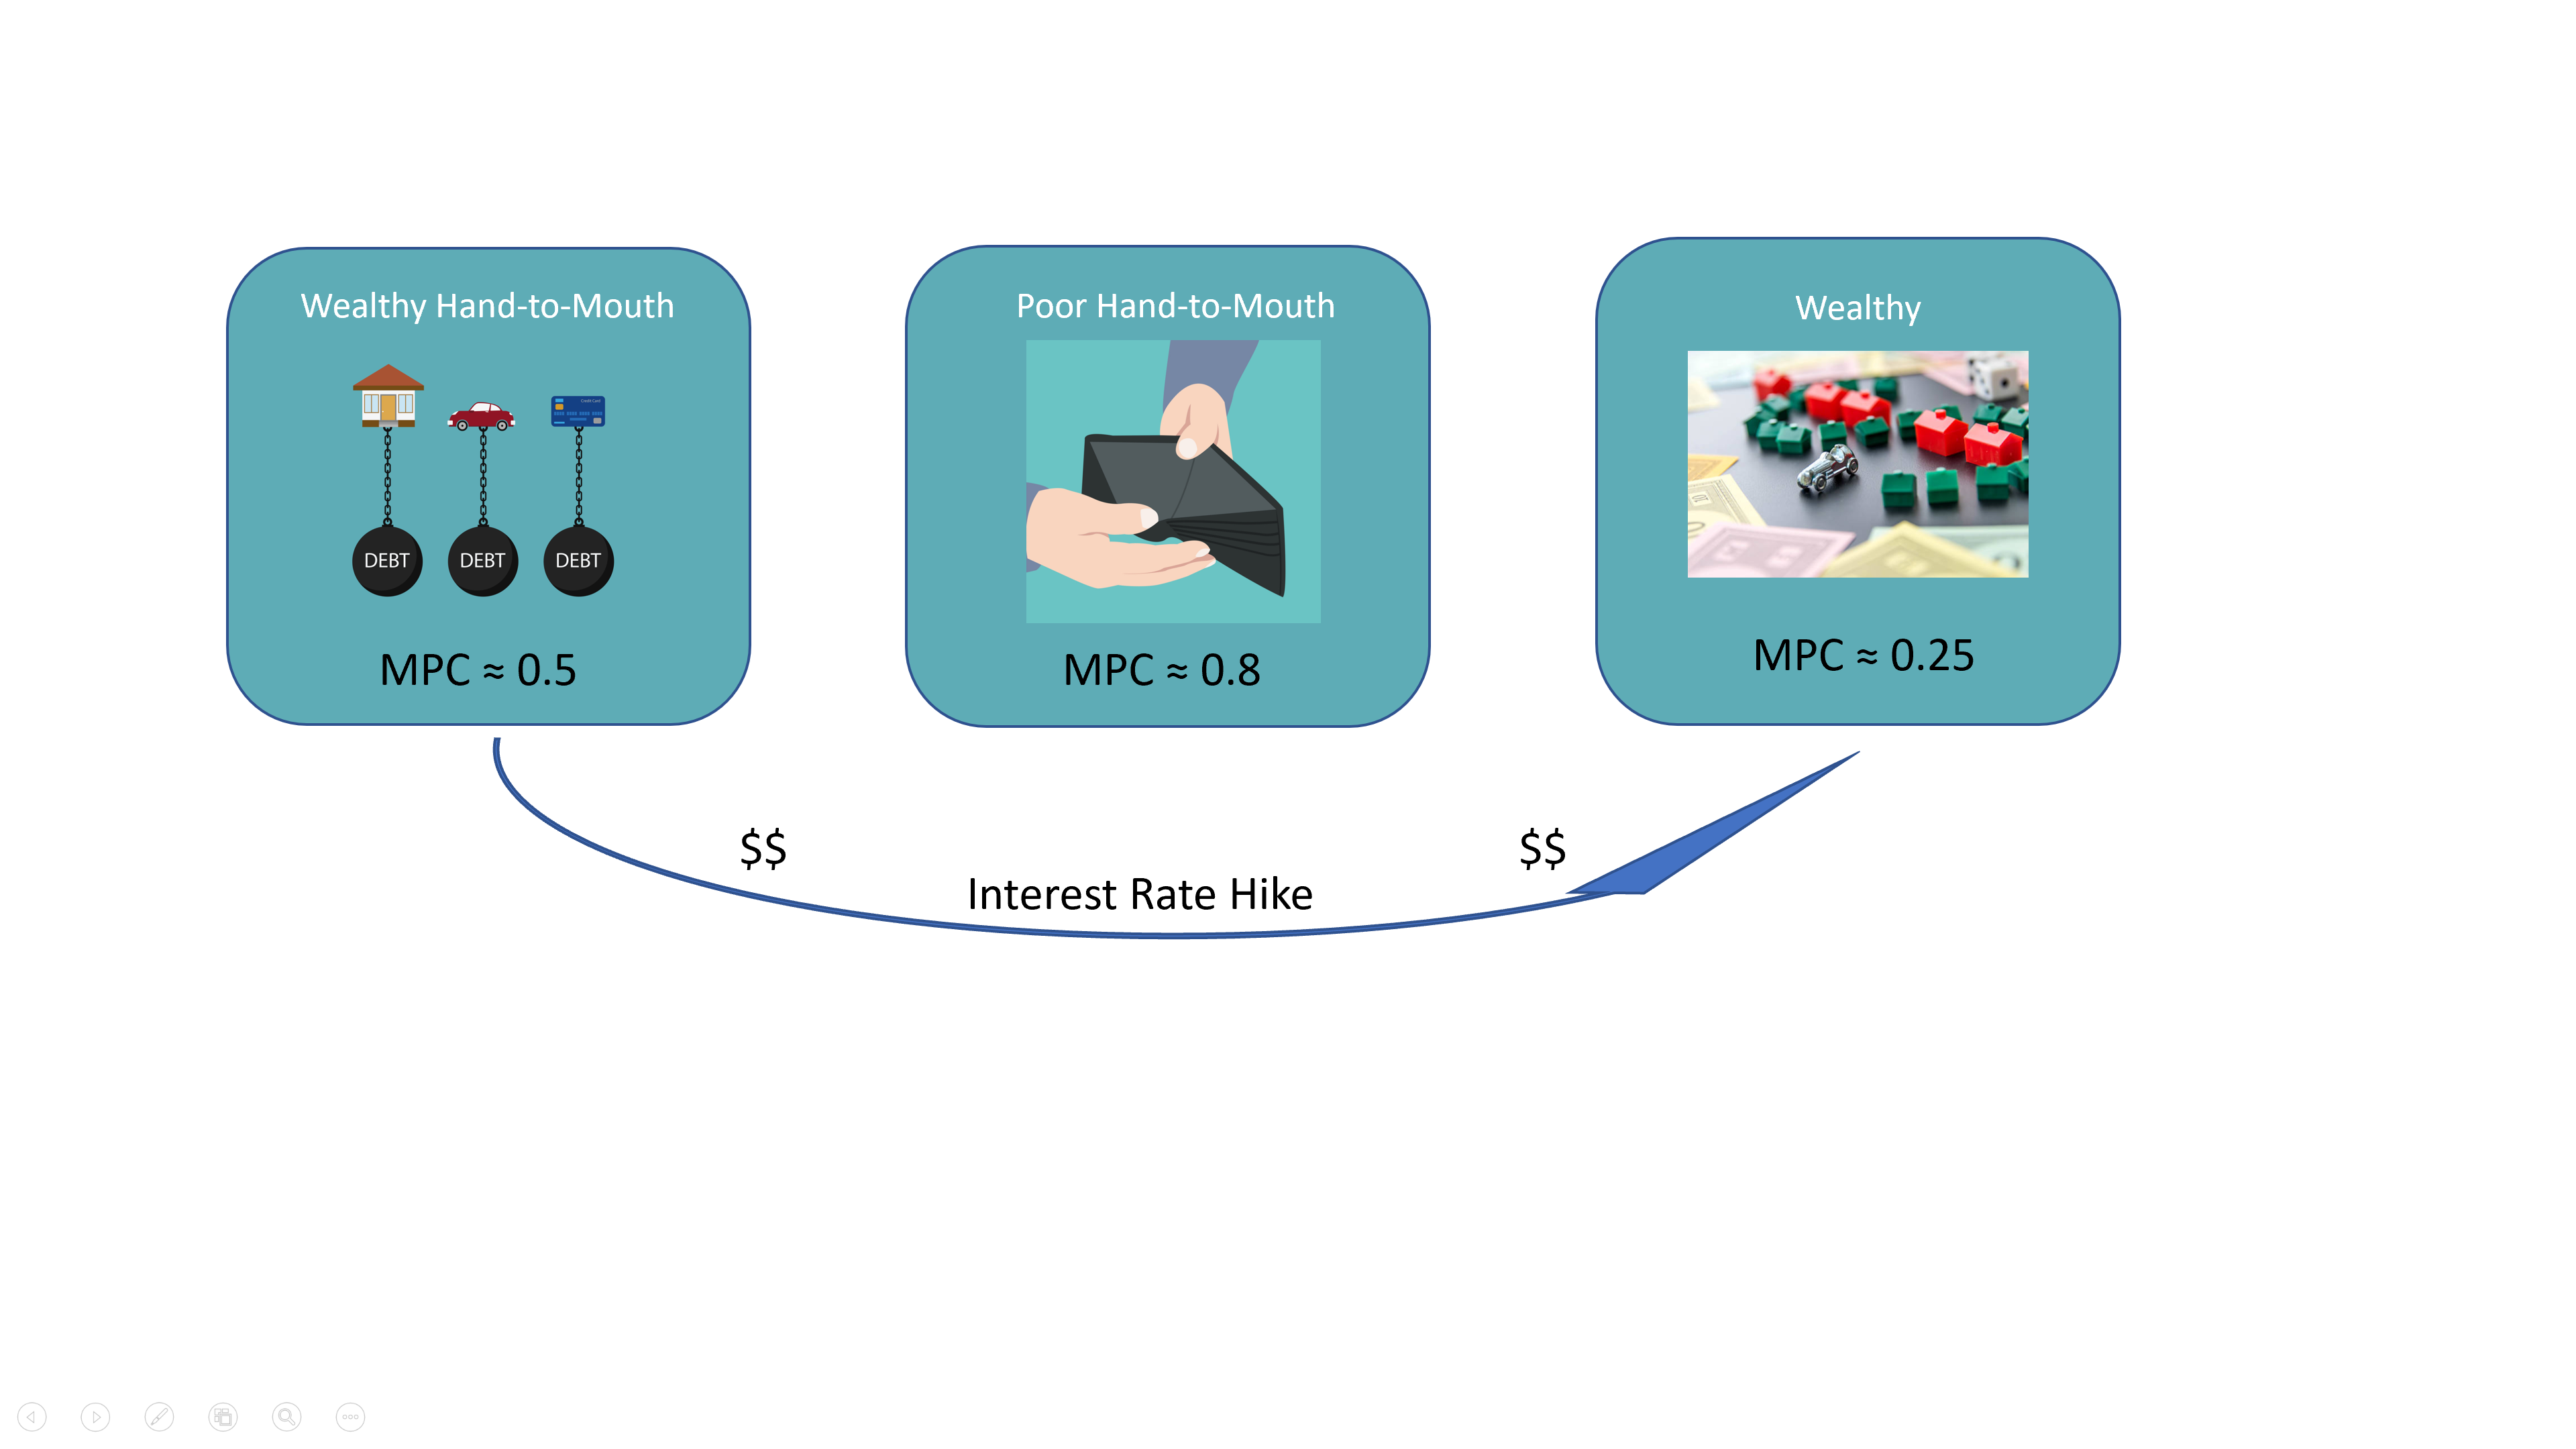
\includegraphics[height=6cm,trim= 3cm 1.9cm 0 3.5cm, clip]{./SlideFigures/IRE3.png}};
%	\pause
%	\node (img4) {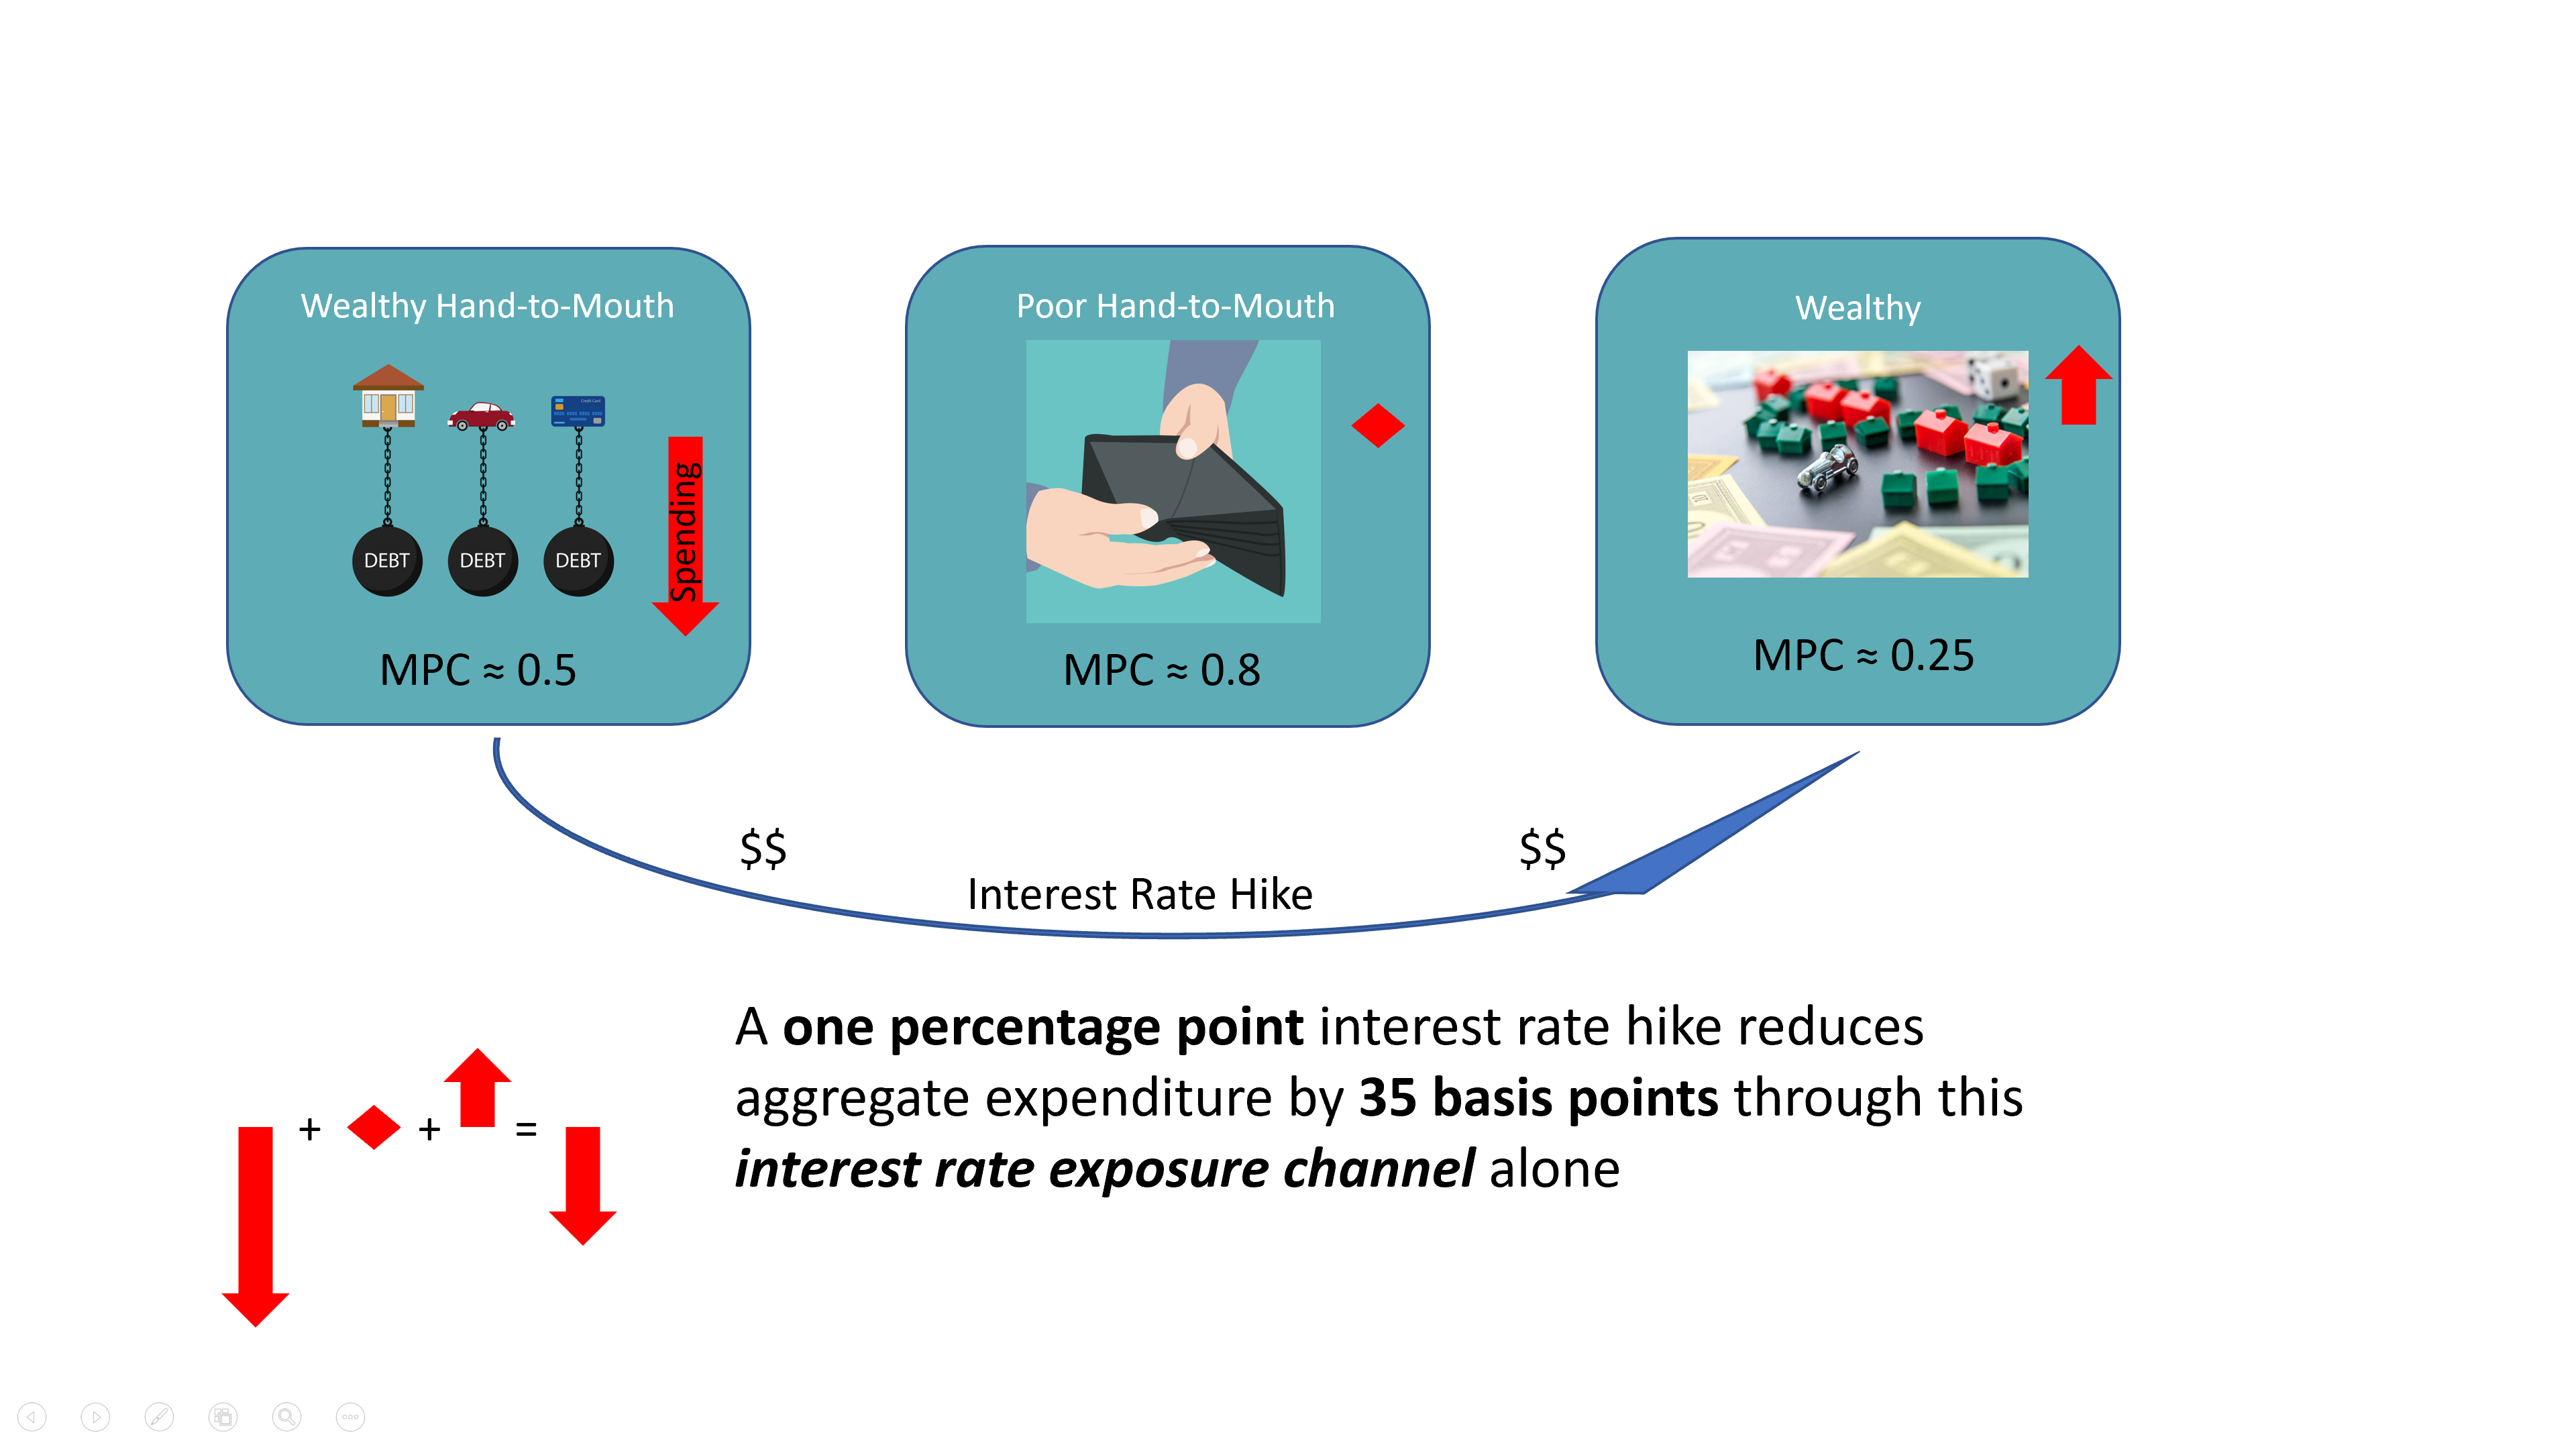
\includegraphics[height=6cm,trim= 3cm 1.9cm 0 3.5cm, clip]{./SlideFigures/IRE5.png}};
	\pause
	\node (img5) {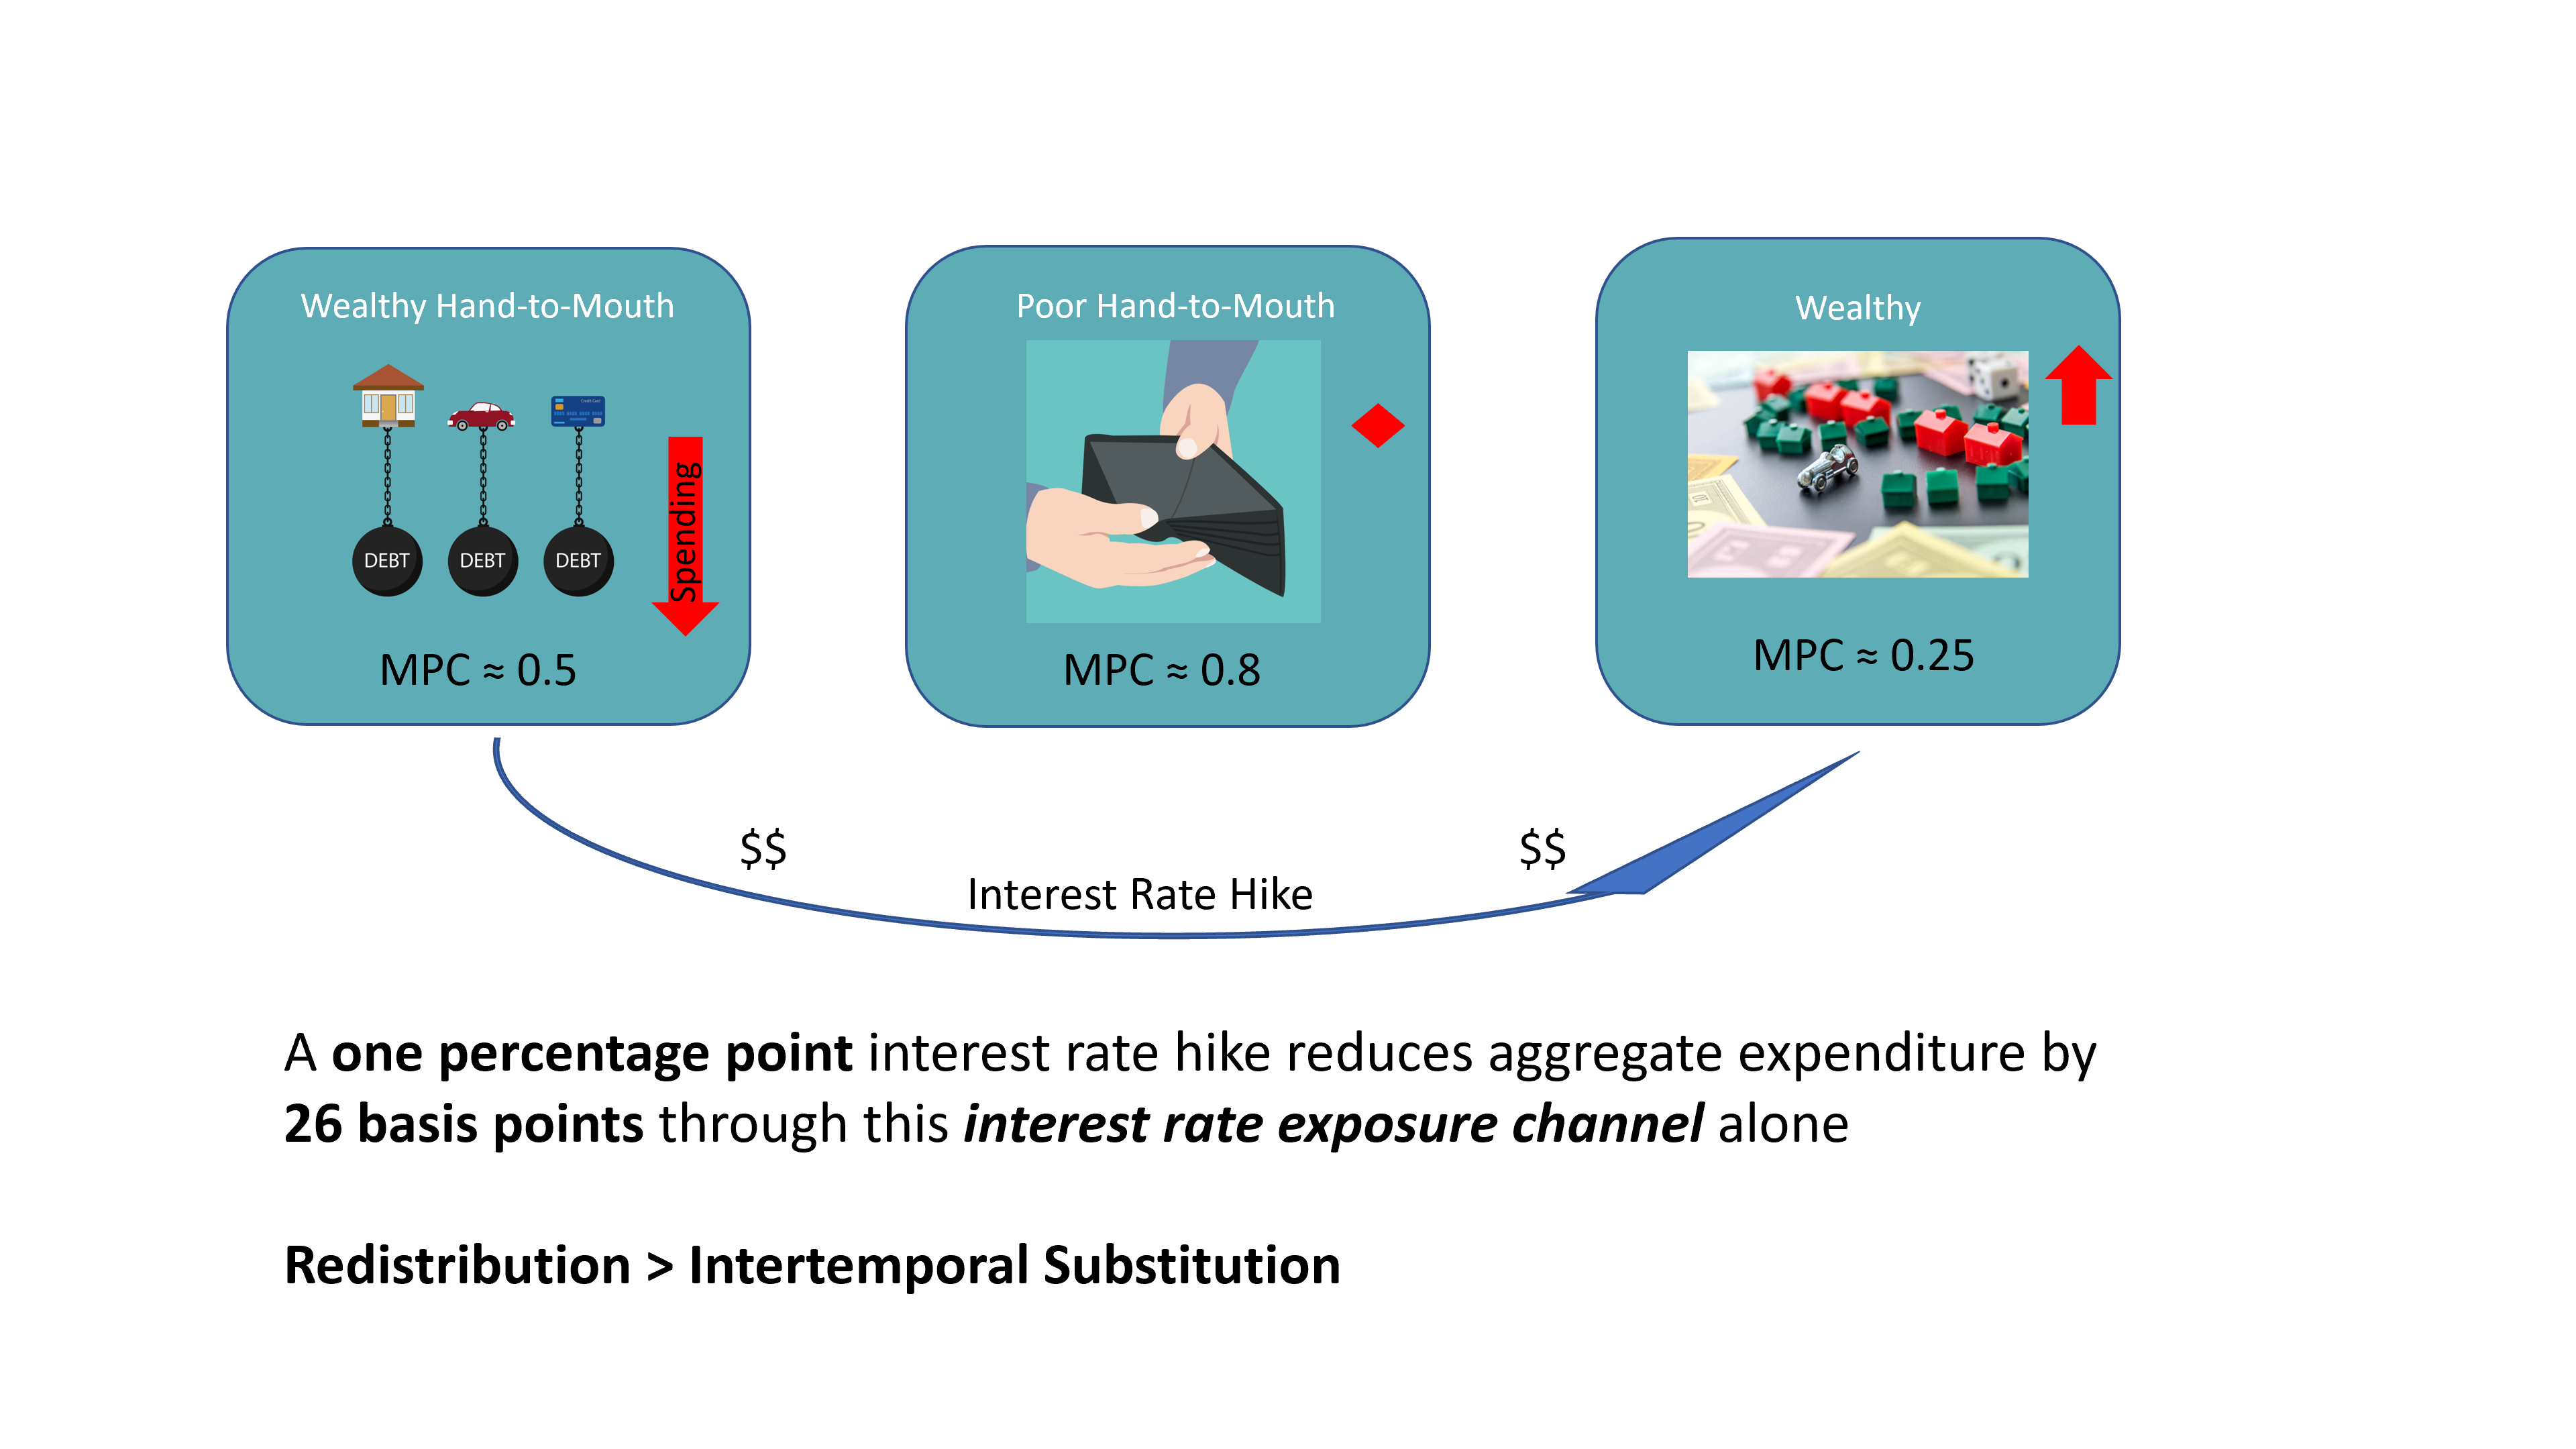
\includegraphics[height=6cm,trim= 3cm 1.9cm 0 3.5cm, clip]{./SlideFigures/IRE6.png}};
	\end{tikzpicture}
}
\frame{
	\frametitle{What has the Empirical MPC literature Found?}
	General consensus: \textbf{MPCs are large} ($\approx 0.5$ including durables)\\
	\begin{itemize}
		\item For both expected and unexpected transitory shocks
	\end{itemize}
	\pause
	\bigskip
	Few studies have enough power to say much about the distribution of MPCs in the population
	\begin{itemize}
		\item \cite{jappelli_fiscal_2014} Italian Survey Data
		\item \cite{fuster_what_2018} NY Fed Survey
		\item \cite{fagereng_mpc_2016} Norway Lottery Data
		\item \cite{gelman_what_2016} Financial App Data
	\end{itemize}
	\bigskip
	\textbf{Liquid assets} and \textbf{income} are key predictors of transitory MPC \\
	\bigskip
	Our method and data can uncover detailed heterogeneity - Many potential applications
}
\section{Empirical Strategy}
\setbeamercovered{invisible}
\frame{
	\frametitle{How Are Consumption Responses Typically Measured?}
	Three methods:
	\begin{itemize}
		\item[1] (Natural) Experiments - stimulus checks, lotteries etc
		\begin{itemize}
			\item Few true experiments, especially for permanent shocks
			\item Data limitations
		\end{itemize}
		\item[2] Ask people
		\begin{itemize}
			\item Unclear how to interpret
		\end{itemize}
		\item[3] Make identifying restrictions on income and consumption dynamics
		\begin{itemize}
			\item Empirical methods (until now!) have been flawed
		\end{itemize}
	\end{itemize}
	\bigskip
	We develop a robust method based on 3
	\bigskip
	
	\hyperlink{BPP}{\beamerbutton{Relation to BPP}}
}



\frame
{
	\frametitle{Identification: Income}
	Income flow consists of:
	\begin{itemize} 
		\item Permanent Income (random walk)
		\item Transitory Income (persistence $<$ 2 years)
	\end{itemize}
    \begin{align*}
	\only<1->{\bar{y}_T  &= \int_{T-1}^{T} p_t dt + \int_{T-1}^{T} \int_{t-2}^{t} f(t-s)dq_s dt \\[7pt]
	 }
	\end{align*}
	\begin{align*}
		\implies \mathrm{Var}(\Delta^N \bar{y}_T) &= (N-\frac{1}{3})\sigma^2_p +  2 \sigma^2_{\tilde{q}} \text{   for }N \geq 3 
			\end{align*}
			\hyperlink{Income_process}{\beamerbutton{Details on income process}}
}
\frame
{
\frametitle{Identification: Consumption}
Assumptions on Consumption\\
	\begin{itemize}
		\item Permanent: Consumption permanently moves by fraction $\phi$ of the income shock
		\item Transitory: Persistence $<$ 2 years
		\end{itemize}
			\begin{align*}
	c_t  &= \phi p_t  + \int_{t-2}^{t} g(t-s)dq_s  \\
	\implies \mathrm{Cov}&(\Delta^N \bar{c_T},\Delta^N \bar{y_T} ) = \phi (N-\frac{1}{3}) \sigma^2_p + 2 \psi \sigma^2_{\tilde{q}}
	\end{align*}
	where  $\psi = \frac{\mathrm{Cov}(\tilde{c},\tilde{q})}{\mathrm{Var}(\tilde{q})}$, the regression coefficient of `transitory' consumption on transitory income \\
		\hyperlink{cons_identification}{\beamerbutton{Consumption identification}}
}		

\frame
{
	\frametitle{Full Identification}
We use GMM on the equations:
\begin{align*}
\mathrm{Var}(\Delta^N \bar{y_T} ) &=  (N-\frac{1}{3}) \sigma^2_p + 2  \sigma^2_{\tilde{q}} \\
\mathrm{Cov}(\Delta^N \bar{c_T},\Delta^N \bar{y_T} ) &= \phi (N-\frac{1}{3}) \sigma^2_p + 2 \psi \sigma^2_{\tilde{q}}
\end{align*}
with $N=3,4,5$ (and $T=2007,..,2015$) to identify the four unknowns:
\begin{itemize}
	\item $\sigma^2_p$: Permanent shock variance
	\item $\sigma^2_{\tilde{q}}$: (Time aggregated) transitory shock variance
	\item $\phi$: MPX out of permanent income shocks
	\item $\psi$: MPX out of transitory income shocks
\end{itemize}
	\textbf{M}arginal \textbf{P}ropensity to e\textbf{X}pend (includes durables)
\hyperlink{Intuition}{\beamerbutton{Methodology intuition}}
}
\section{Data}
\frame
{
	\frametitle{Data}
	What we need:
	\begin{itemize}
		\item Panel Data on Income and Expenditure
		\item Household Balance Sheet Data (detail on nominal assets)
	\end{itemize}
	\pause
	Income:
	\begin{itemize}
		\item Starting point: Register based micro data for all Danish households made available by Statistics Denmark
		\begin{itemize}
			\item We use after-tax income for the household head, based on third-party reported tax data
			\item Restrict sample to heads aged 30-55
		\end{itemize}
		\item We divide through by permanent income (mean income over all observed years) and take the residual after controlling for age, education, marital status etc. (along with interactions of these)
	\end{itemize}
}
\frame
{
	\frametitle{Data: Expenditure}
	We impute expenditure from the budget constraint
		\begin{align*}
			C_t \equiv Y_t - S_t = Y_t - P_t - \Delta NW
		\end{align*}
	\begin{itemize}
		\item Deposit and brokerage accounts all third party reported
		\item Works well for households with simple financial lives
		\item Main issue: Capital gains and losses
		\begin{itemize}
			\item Exclude households where methodology will not work well (eg business owners)
			\item Exclude housing wealth and years with housing transactions
			\item Capital gains for stocks based on a diversified index
		\end{itemize}
		\item Noisy, but perhaps better than surveys (\cite{abildgren_consistency_2018})
		\item Huge sample size advantage: sample covers 7.6 million observations over 2004-2015
	\end{itemize}
		\hyperlink{measurement_error}{\beamerbutton{On measurement error}}
}

\section{Liquid Wealth}
\frame
{
	\frametitle{Results by Liquid Wealth}
	\label{MPXbyLiquidWealth}
	\begin{columns}
		\column{0.5\linewidth}
		\centering
		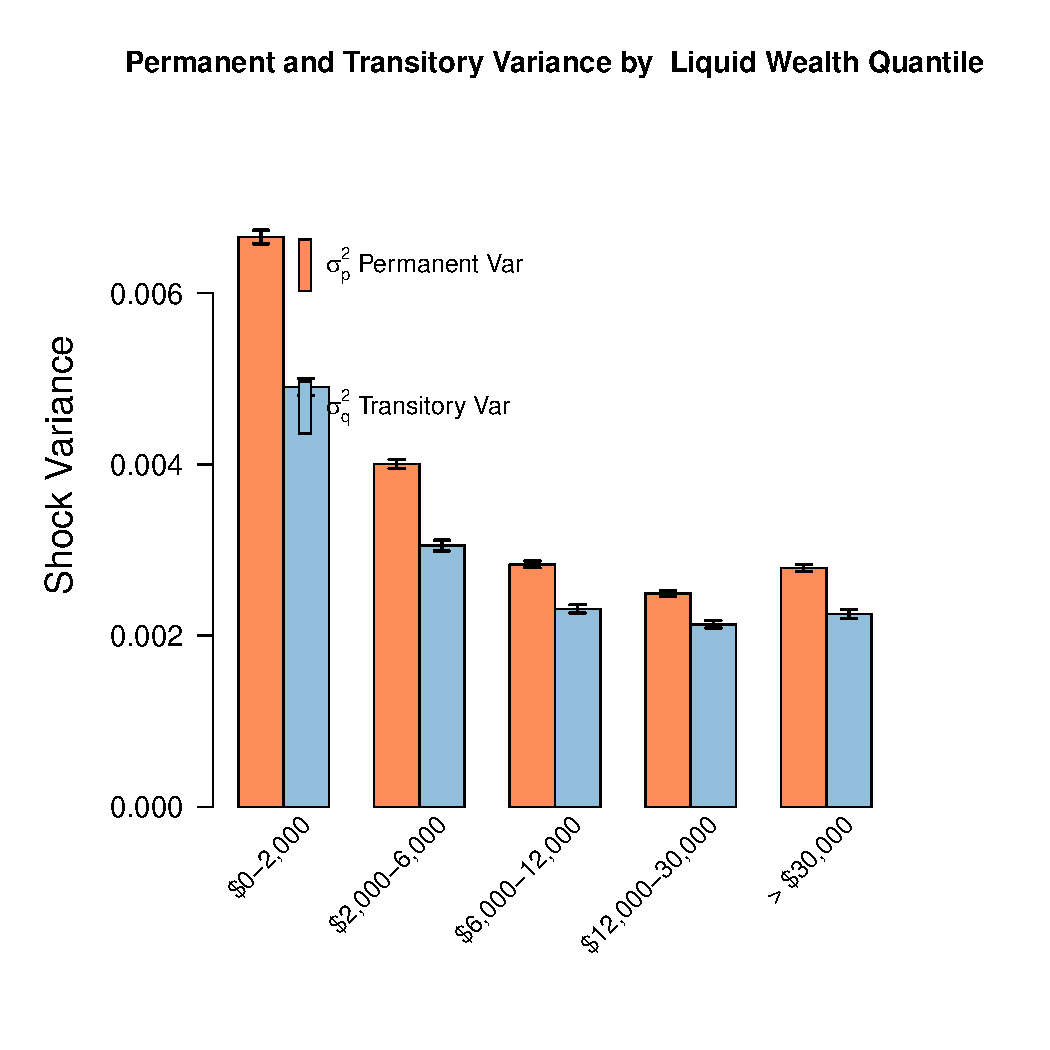
\includegraphics[scale=0.35]{../Figures/VarianceByLiquidWealth_level_lincome_head.pdf}
		\column{0.5\linewidth}
		\centering
		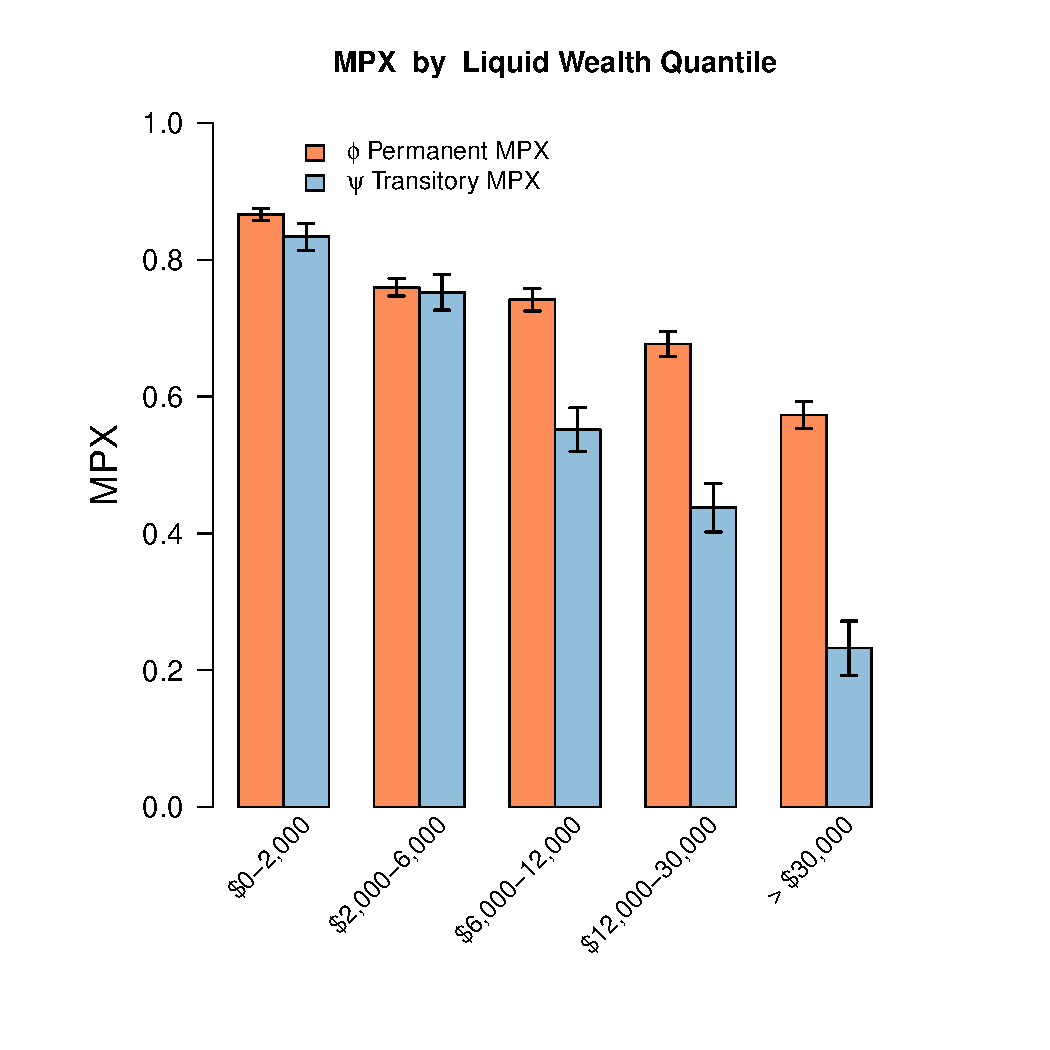
\includegraphics[scale=0.35]{../Figures/MPXByLiquidWealth_level_lincome_head.pdf}
	\end{columns} 
	\hyperlink{MPXbyNetWealth}{\beamerbutton{MPX by Net Wealth}}	
}

\section{Monetary Policy}
\frame{
	\frametitle{Monetary Policy: Auclert's Decomposition}
	How does Monetary Policy Effect Aggregate Consumption?\\
	\bigskip
	\begin{itemize}
		\item Intertemporal Substitution \tikz[baseline]{\node(topbrace1){}}
		\item Aggregate Income \tikz[baseline]{\node(bottombrace1){}}
	\begin{tikzpicture}[overlay, remember picture]
	\draw [decoration={brace,amplitude=0.5em},decorate,ultra thick,black]
	let \p1=(topbrace1), \p2=(bottombrace1) in
	({max(\x1,\x2)+1.8em}, {\y1+0.8em}) -- node[right=0.6em] {Representative Agent Channels} ({max(\x1,\x2)+1.8em}, {\y2});
	\end{tikzpicture}
	\pause
	\only<2>{
	\begin{tikzpicture}[remember picture,overlay]
	\node (topbrace1a)  at ([shift={(-5,0.1)}]topbrace1) {};
	\node (topbrace1b)  at ([shift={(-5,1.8)}]topbrace1) {};
	\node (bottombrace1a)  at ([shift={(-3.7,0.1)}]bottombrace1) {};
	\node (bottombrace1b)  at ([shift={(-3.7,-0.7)}]bottombrace1) {};
	\draw[blue,thick,->] (topbrace1a)  to [in=180,out=180] (topbrace1b) node[anchor=west,text = blue] {Dominates in Rep. Agent NK models};
	\draw[blue,thick,->] (bottombrace1a)  to [in=180,out=180] (bottombrace1b) node[anchor=west,text = blue] {Large in Spender-Saver, or TANK models};
	\end{tikzpicture}
	}
		\pause
		\item Fisher (Inflationary debt relief) \tikz[baseline]{\node(topbrace2){}}
		\item Earnings Heterogeneity
		\item Interest Rate Exposure \tikz[baseline]{\node(m1){}}
	\begin{tikzpicture}[overlay, remember picture]
\draw [decoration={brace,amplitude=0.5em},decorate,ultra thick,black]
let \p1=(topbrace2), \p2=(m1) in
({max(\x1,\x2)}, {\y1+0.8em}) -- node[right=0.6em] {Redistribution Channels} ({max(\x1,\x2)}, {\y2});
\end{tikzpicture}
	\end{itemize}
	\bigskip
	\pause
	How can we \textit{empirically} measure the size of the redistribution channels?\\
	\bigskip
	Need to know the distribution of MPCs along the relevant dimension of redistribution
}
\frame{
	\frametitle{Interest Rate Exposure: Auclert's Experiment}
	\begin{itemize}
		\item Real interest rate increases 1\% for 1 year
		\item Hold constant income and inflation
	\end{itemize}
	\bigskip
	How does the subsequent redistribution impact aggregate consumption?\\
	\bigskip
	Dimension of Redistribution: Unhedged Interest Rate Exposure
}
\frame{
	\frametitle{Interest Rate Exposure: Dimension of Redistribution}
	Define \textbf{Unhedged Interest Rate Exposure} for household $i$ as the total savings the household will invest at this year's interest rate:
	\begin{align*}
	URE_i = Y_i - C_i + A_i - L_i
	\end{align*}
	Where
	\begin{itemize}
		\item $Y_i = $ Total after tax income 
		\item $C_i = $ Total Expenditure, including interest payments
		\item $A_i = $ Maturing assets
		\item $L_i = $ Maturing liabilities
	\end{itemize}
	Following a change in the interest rate $dR$, the size of the Interest Rate Exposure channel on household $i$'s expenditure is:
	\begin{align*}
		dc_i = MPC_i URE_i  \frac{dR}{R}
	\end{align*}
}
\frame{
	\frametitle{Interest Rate Exposure: Aggregation}
	Aggregate to find size of channel:
	\begin{align*}
	dc_i &= \quad \ \ MPC_i URE_i  \ \ \ \frac{dR}{R} \\
	\implies \frac{dC}{C} &= \mathbb{E}_I \Big(MPC_i \frac{URE_i}{\mathbb{E}_I (c_i)}   \Big) \frac{dR}{R} 
	\end{align*}
	Define sufficient statistic:
	\begin{align*}
	\mathcal{E}_R  = \mathbb{E}_I \Big(MPC_i \frac{URE_i}{\mathbb{E}_I (c_i)}   \Big) 
	\end{align*}
	\bigskip
	$\implies$ Need to know the distribution of $MPC_i$ with $URE_i$\\
	\bigskip
	We can do that!
}
\frame{
	\frametitle{Interest Rate Exposure: MPX Distribution}
		\begin{center}
		\begin{tikzpicture}
%		\node (img1) {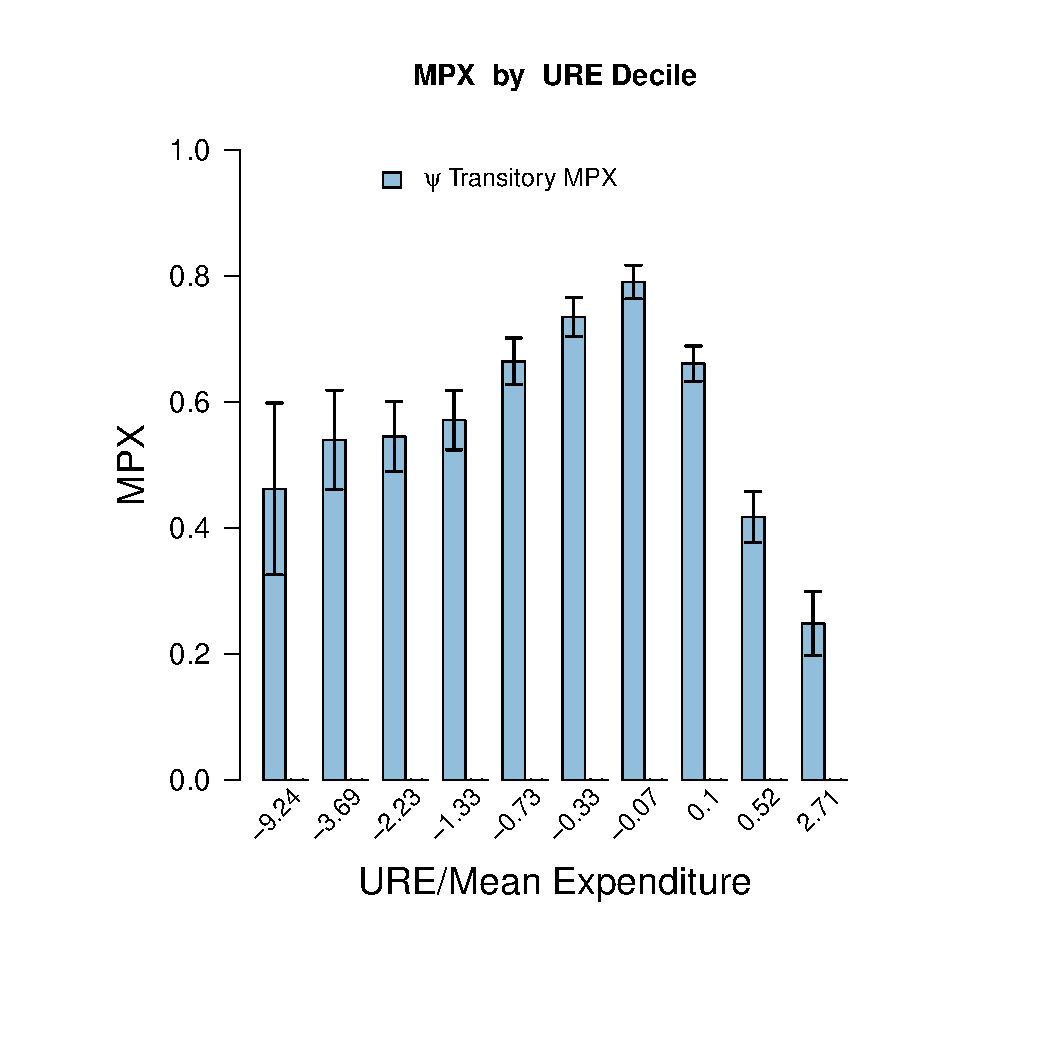
\includegraphics[scale=0.5]{../Figures/MPXByUREdetails1_level_lincome_head.pdf}};
%		\pause
		\node (img2) {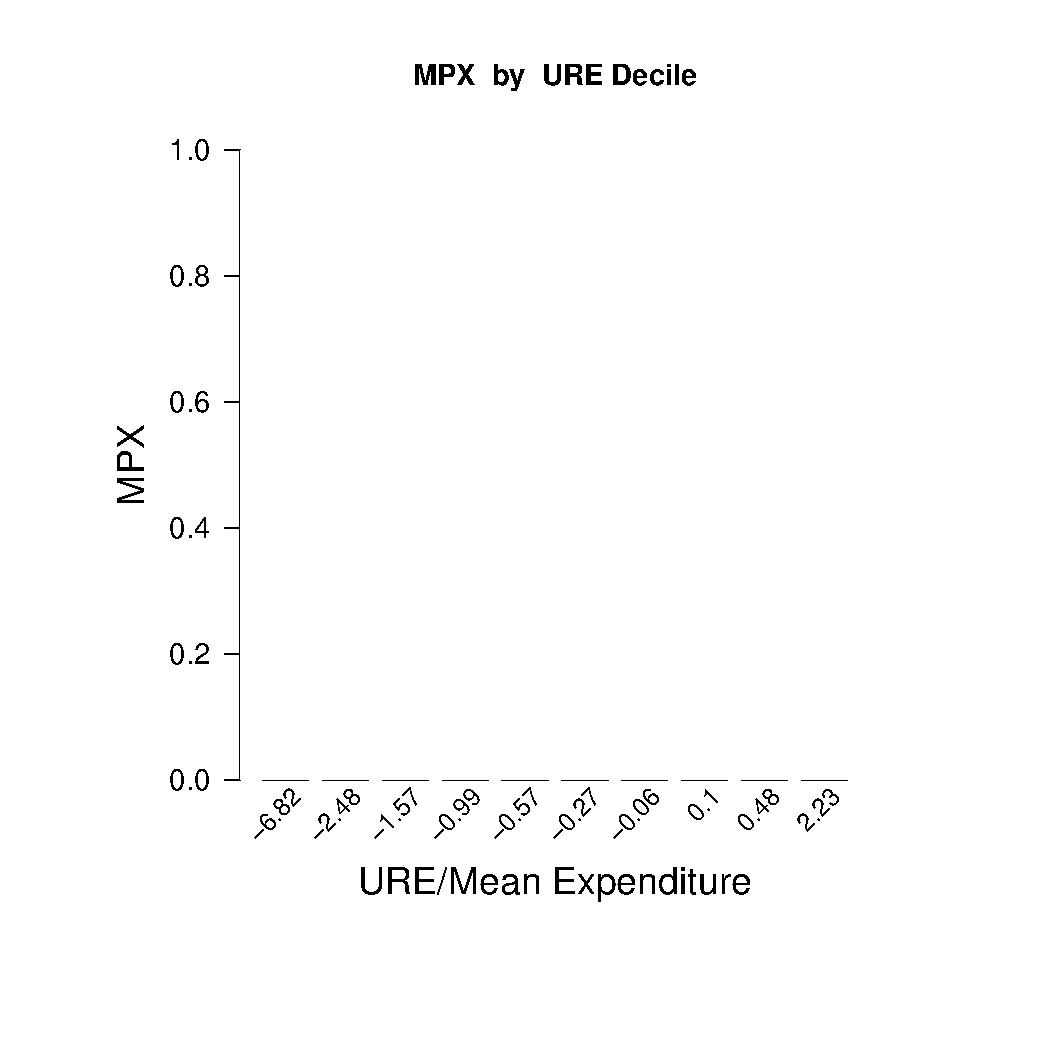
\includegraphics[scale=0.5]{../Figures/MPXByUREdetailsblank_level_lincome_head.pdf}};
		\node (img3)
		{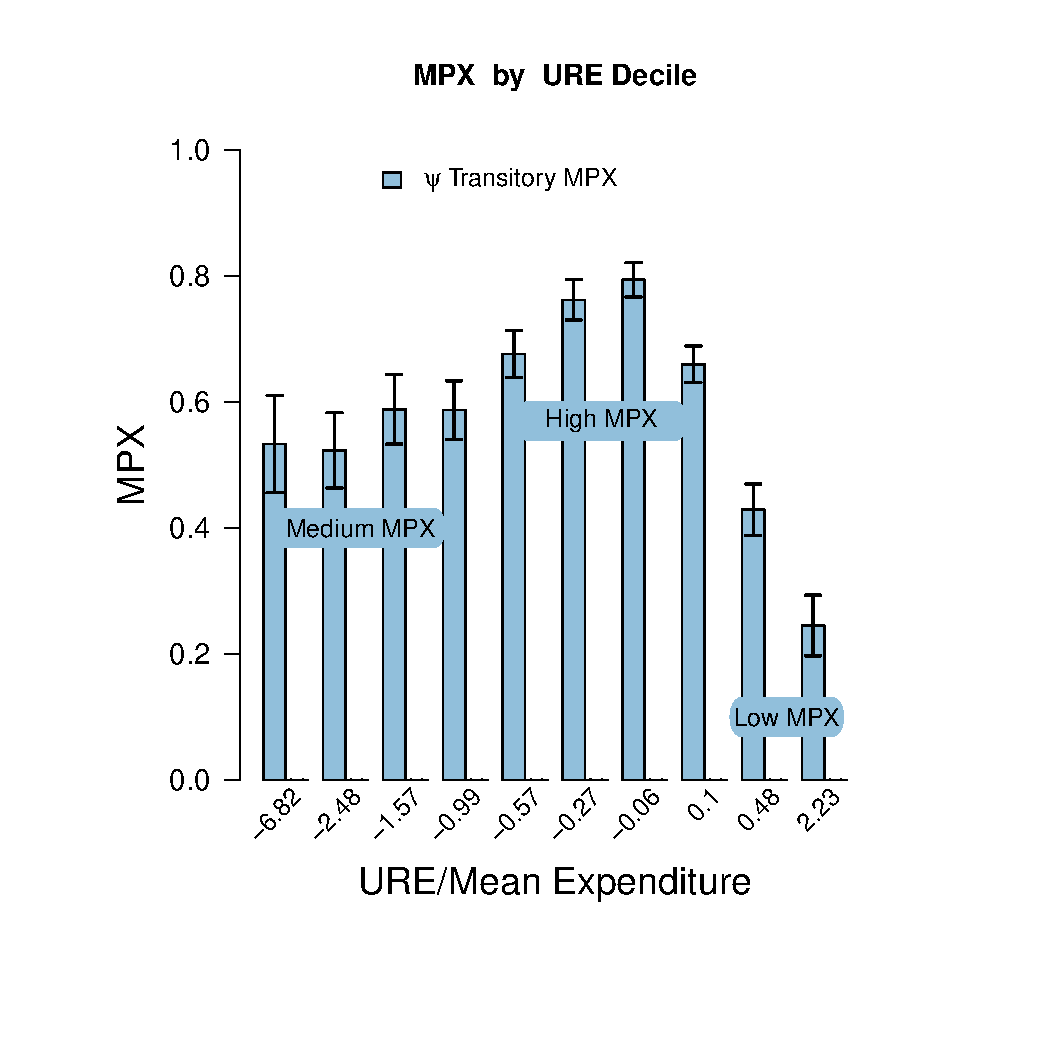
\includegraphics[scale=0.5]{../Figures/MPXByUREdetails1a_level_lincome_head.pdf}};
%		\pause
%		\node (img4) {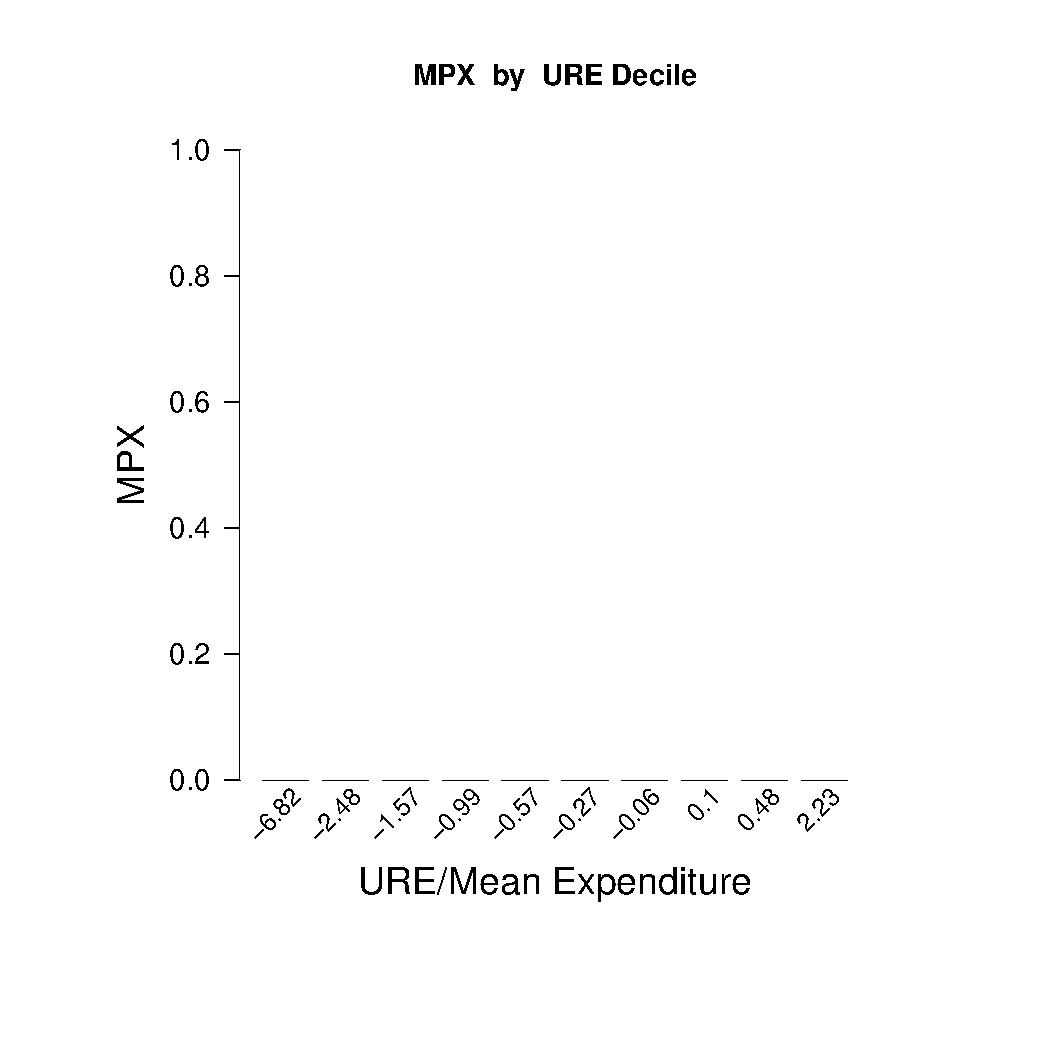
\includegraphics[scale=0.5]{../Figures/MPXByUREdetailsblank_level_lincome_head.pdf}};
%		\node (img5) {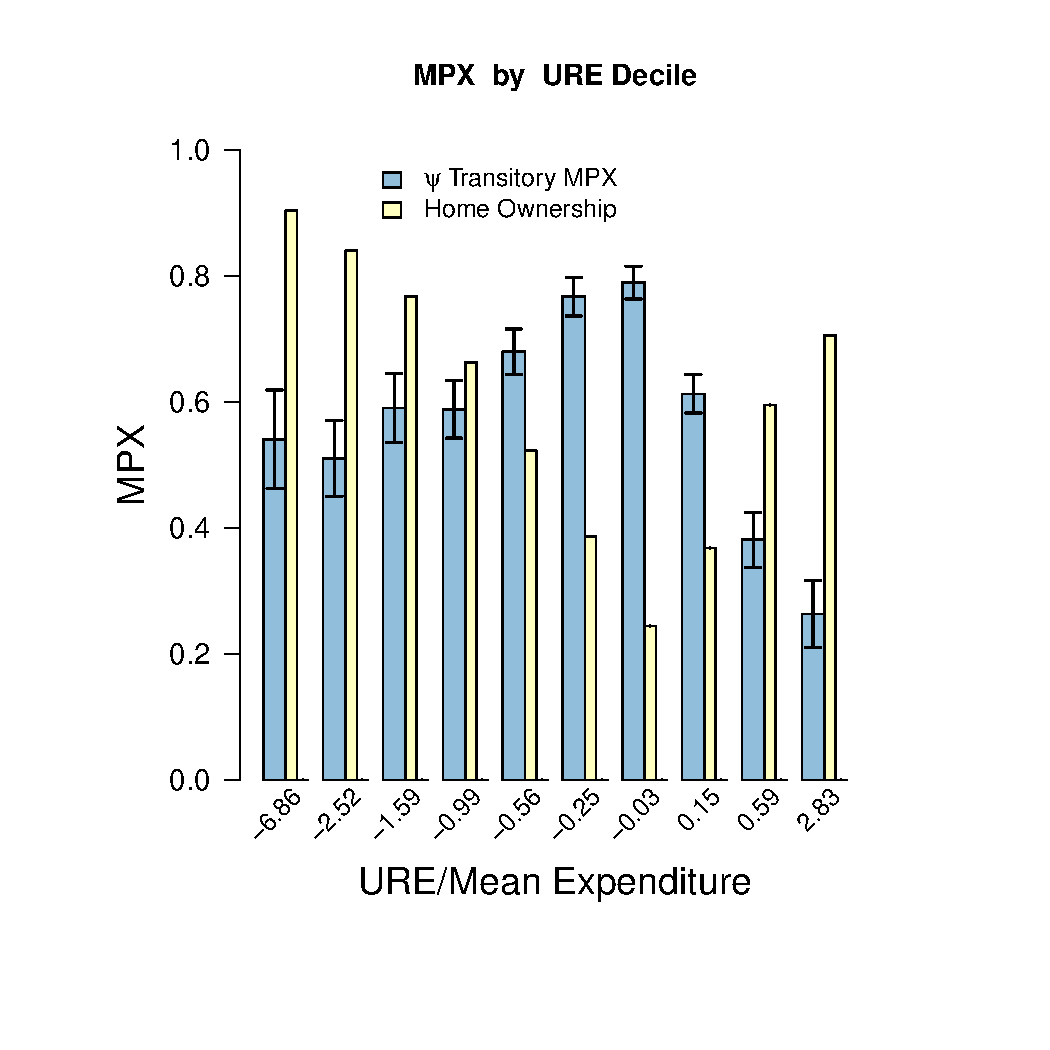
\includegraphics[scale=0.5]{../Figures/MPXByUREdetails2_level_lincome_head.pdf}};
		\pause
		\node (img6) {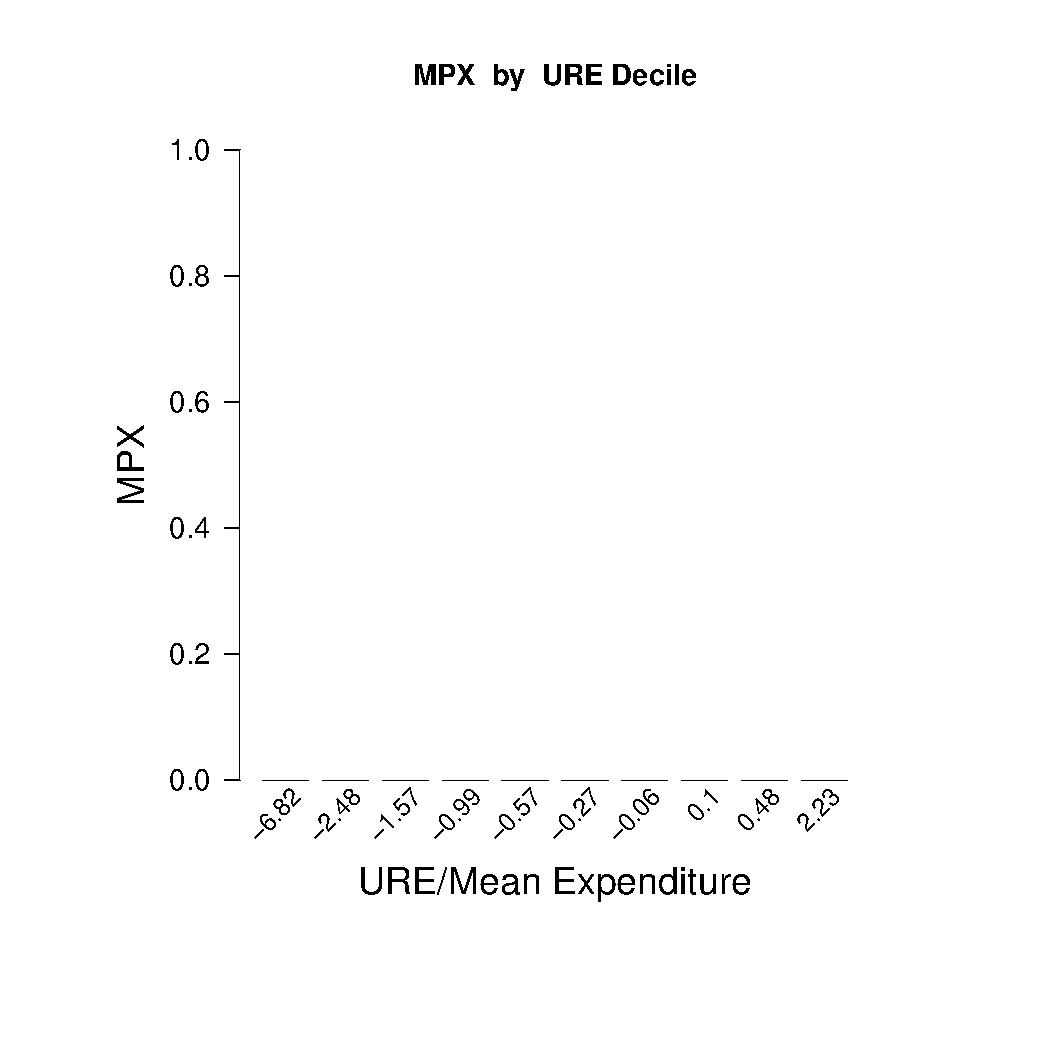
\includegraphics[scale=0.5]{../Figures/MPXByUREdetailsblank_level_lincome_head.pdf}};
		\node (img7)
		{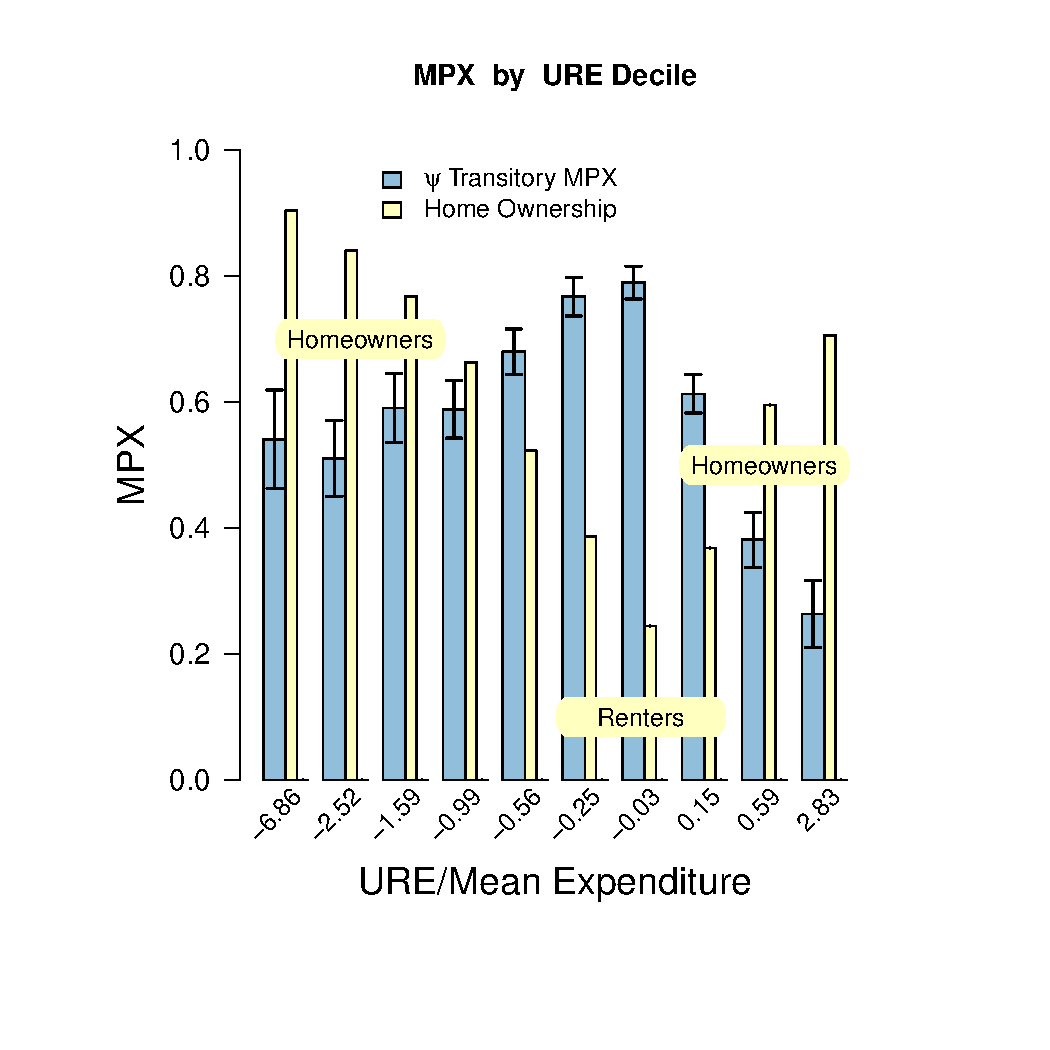
\includegraphics[scale=0.5]{../Figures/MPXByUREdetails2a_level_lincome_head.pdf}};
%		\pause
%		\node (img8) {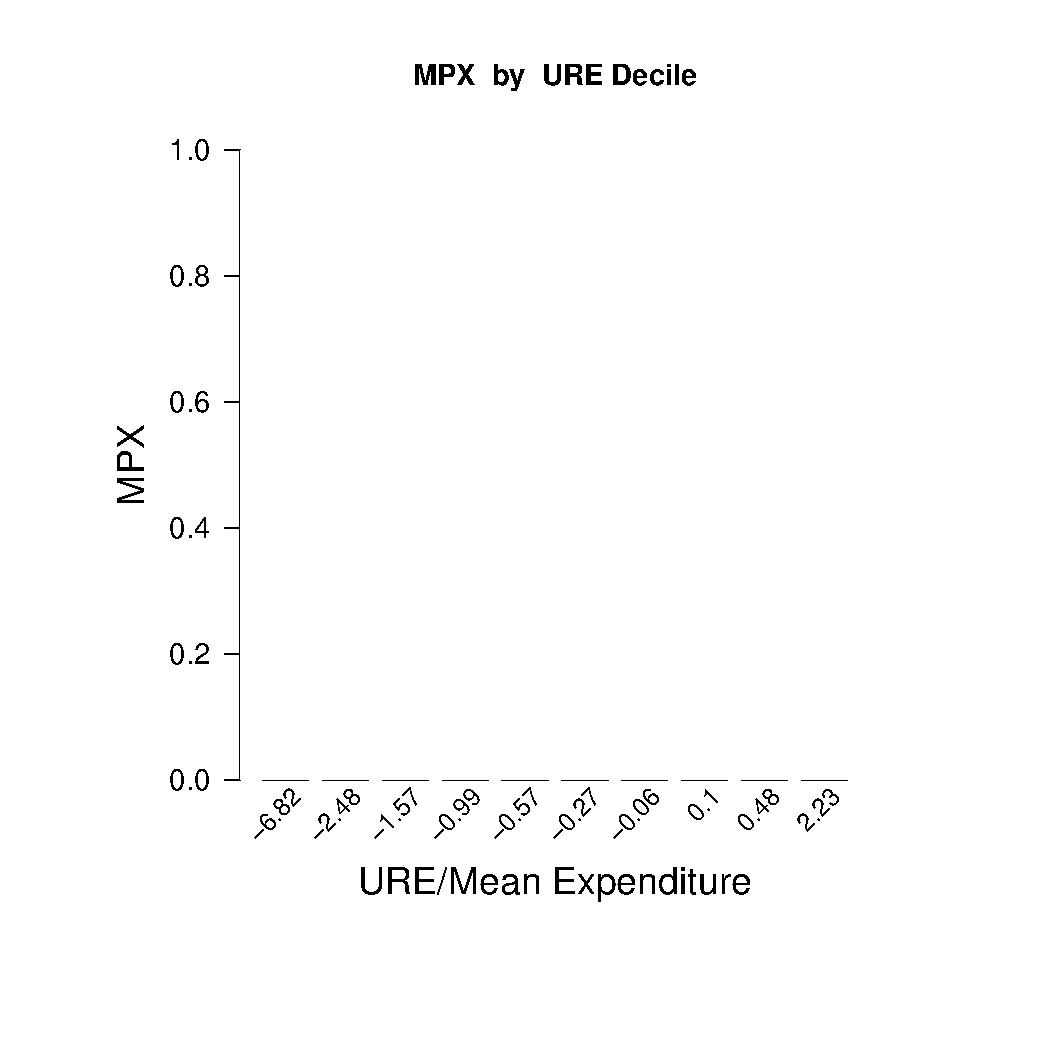
\includegraphics[scale=0.5]{../Figures/MPXByUREdetailsblank_level_lincome_head.pdf}};
%		\node (img9) {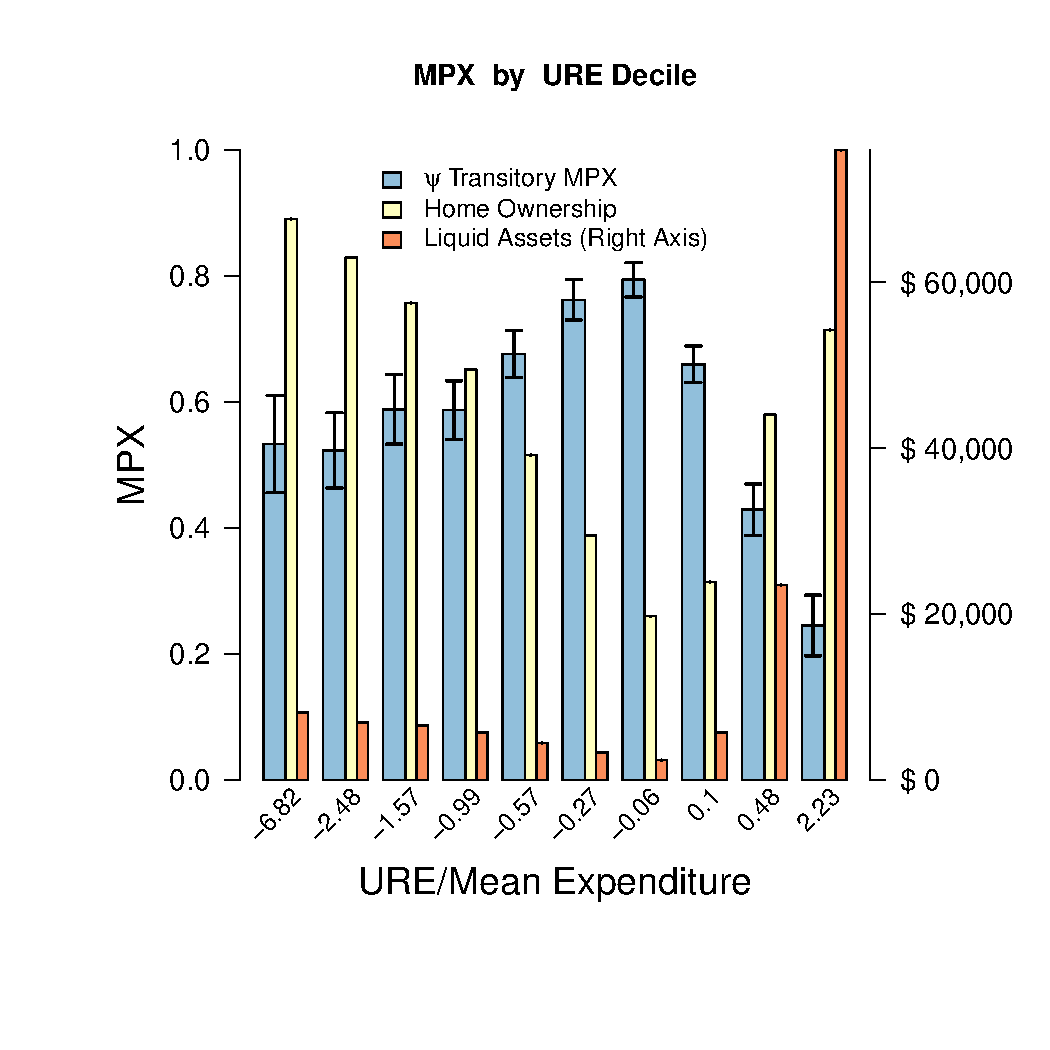
\includegraphics[scale=0.5]{../Figures/MPXByUREdetails3_level_lincome_head.pdf}};
		\pause
		\node (img10) {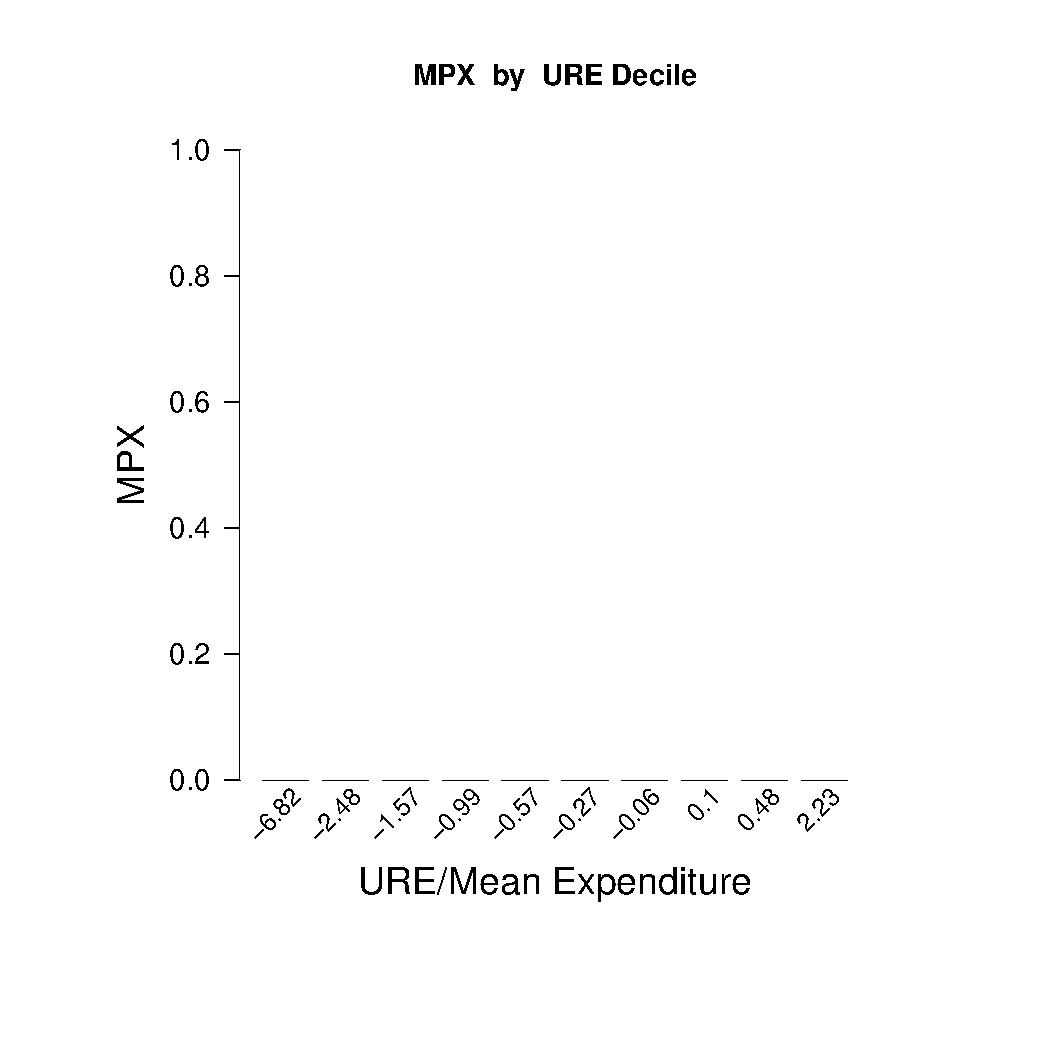
\includegraphics[scale=0.5]{../Figures/MPXByUREdetailsblank_level_lincome_head.pdf}};
		\node (img11) {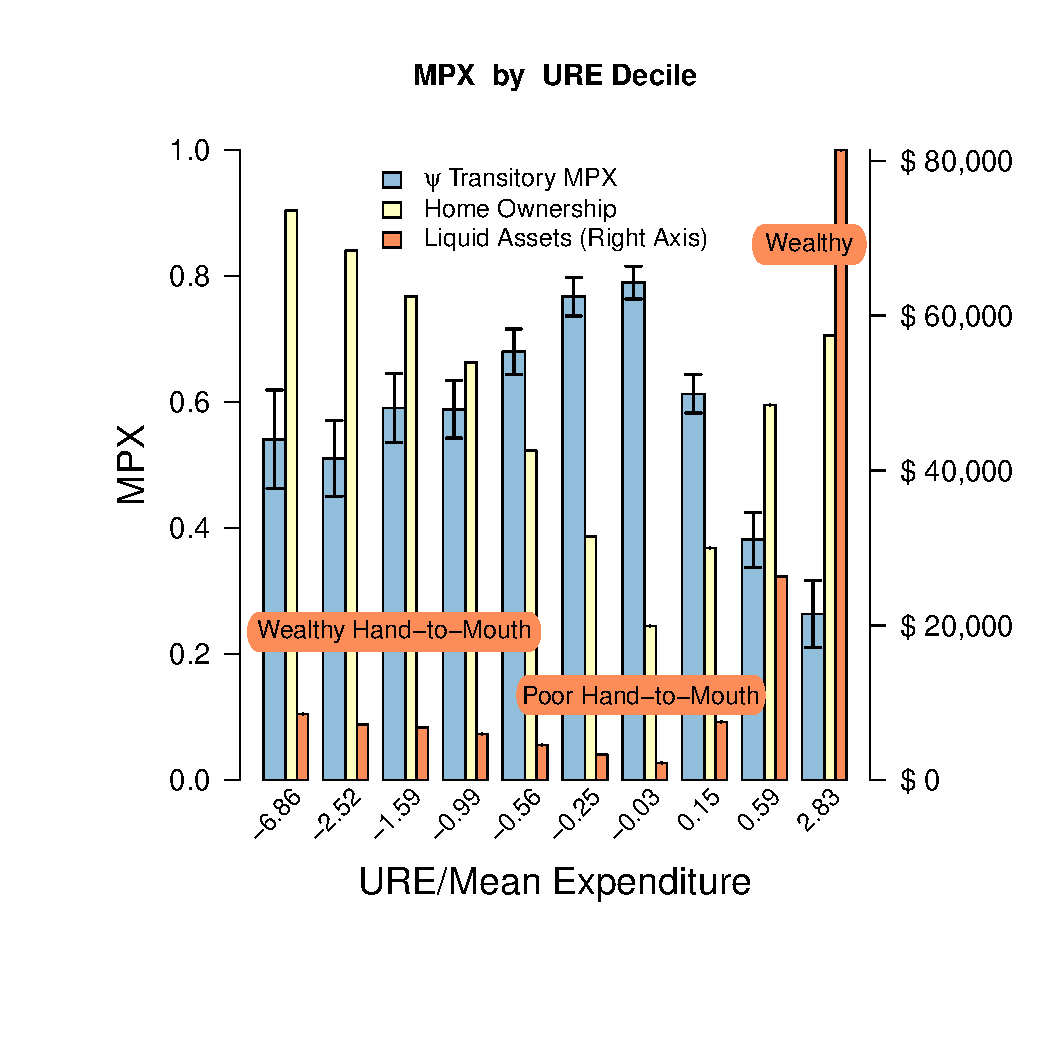
\includegraphics[scale=0.5]{../Figures/MPXByUREdetails3a_level_lincome_head.pdf}};
		\end{tikzpicture}
	\end{center}
}
\frame{
	\frametitle{Interest Rate Exposure: Out of Sample}
	\textit{Total} URE sums to zero - this is not true for our household sample 
	\begin{itemize} 
		\item -57bn USD 
	\end{itemize}
	\bigskip
	\tiny
	\input ../Tables/URE_table.tex
}
\frame{
	\frametitle{All Five Transmission Channels}
	\begin{align*} 
	\frac{dC}{C} &= \overbrace{\mathcal{M}\frac{dY}{Y}}^{\text{Aggregate Income Channel}\qquad} \overbrace{ + \gamma \mathcal{E}_Y \frac{dY}{Y}}^{\text{Earnings Heterogeity Channel}\qquad} \overbrace{ - \mathcal{E}_P\frac{dP}{P}}^{\text{Fisher Channel}}  \nonumber \\
	& \qquad \underbrace{ + \mathcal{E}_R \frac{dR}{R}}_{\text{Interest Rate Exposure Channel}\qquad}  \underbrace{ - \sigma \mathcal{S}\frac{dR}{R}}_{\text{Intertemporal Substitution Channel}} \label{auclert_channels}
	\end{align*}
	\begin{columns}
	\column{0.5\linewidth}
	\centering
		\input ../Tables/sufficient_stats2.tex
	\column{0.5\linewidth}
	\pause
	Compare $\mathcal{E}_R$ to $\sigma S$:\\
	\bigskip
	$\sigma$ in the range of 0.1 to 0.5 (maybe) \\
	\bigskip
	 $\sigma S \approx 0.05 - 0.25$ \\
	\end{columns}

	\begin{tikzpicture}[remember picture,overlay]
	\draw[red,thick] (2.84,0.87) circle (0.45cm);
	\draw[red,thick] (7.1,0.51) circle (0.45cm);
	\end{tikzpicture} 
}
\section{Model}
\frame{
	\frametitle{Aim of Modeling Exercise}
	Can we calibrate a standard Buffer-Stock saving model to fit the distribution of MPC with liquid wealth?
	\begin{columns}
	\column{0.5\linewidth}
	\centering
	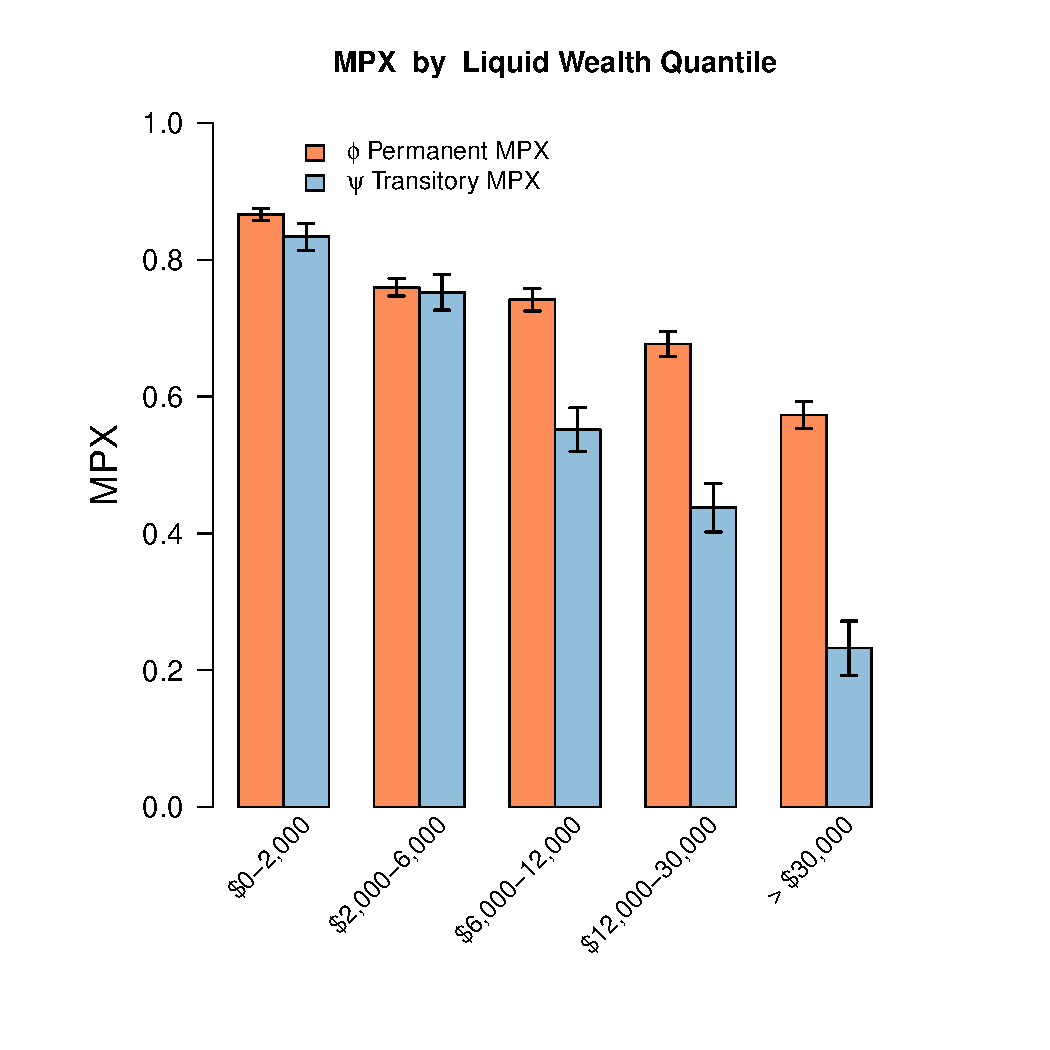
\includegraphics[scale=0.35]{../Figures/MPXByLiquidWealth_level_lincome_head.pdf}
	\column{0.5\linewidth}
	Key features:
	\begin{itemize}
		\item High overall Transitory MPC
		\item Decreasing with liquid wealth
	\end{itemize}
\end{columns}
	\hyperlink{Model}{\beamerbutton{Model details}}
}
\frame
{
	\frametitle{Taste Shock Model: Results}
	\begin{columns}
	\column{0.5\linewidth}
	\centering
	\begin{tikzpicture}
	\node (img1) {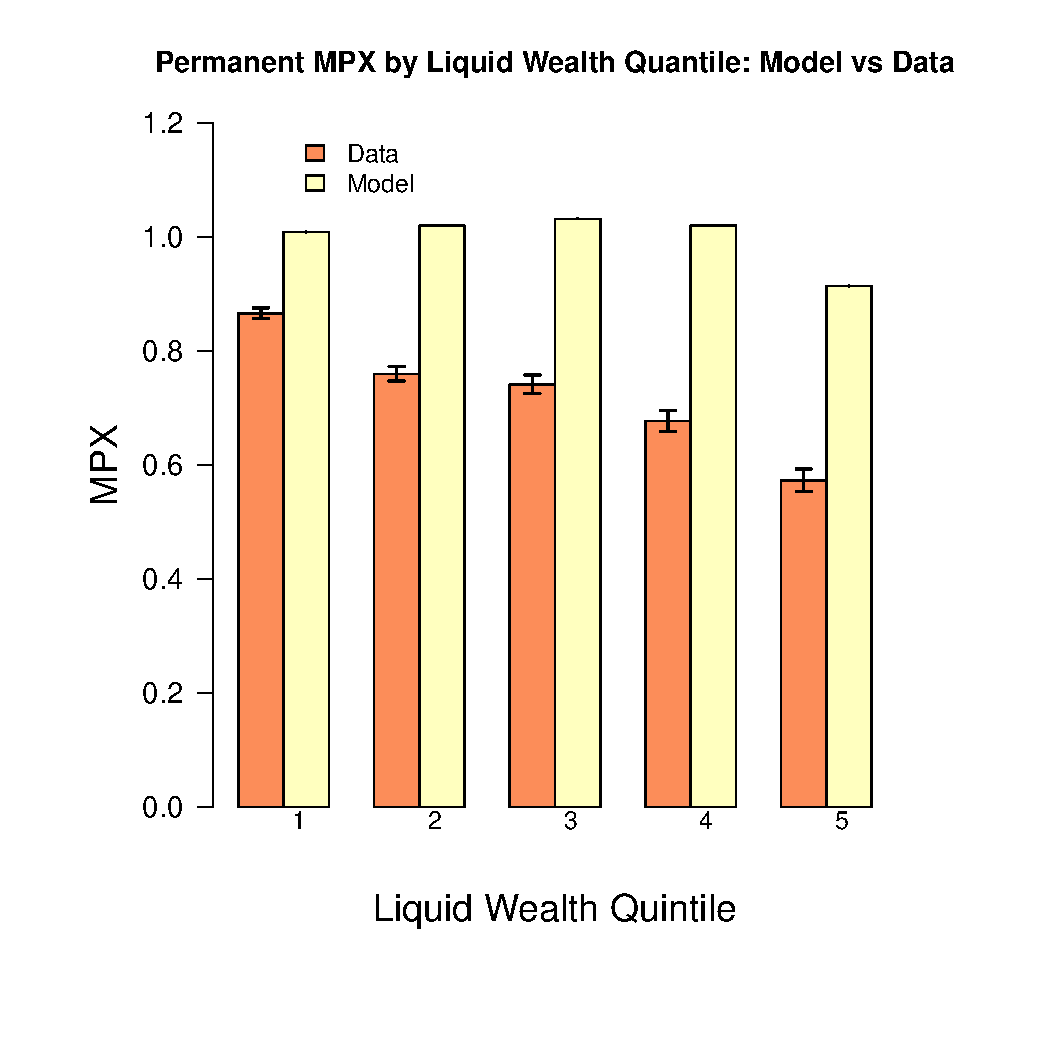
\includegraphics[scale=0.35]{../Figures/CSTW_perm_denmark_pref.pdf}};
	\end{tikzpicture}
	\column{0.5\linewidth}
	\centering
	\begin{tikzpicture}
	\node (img3) {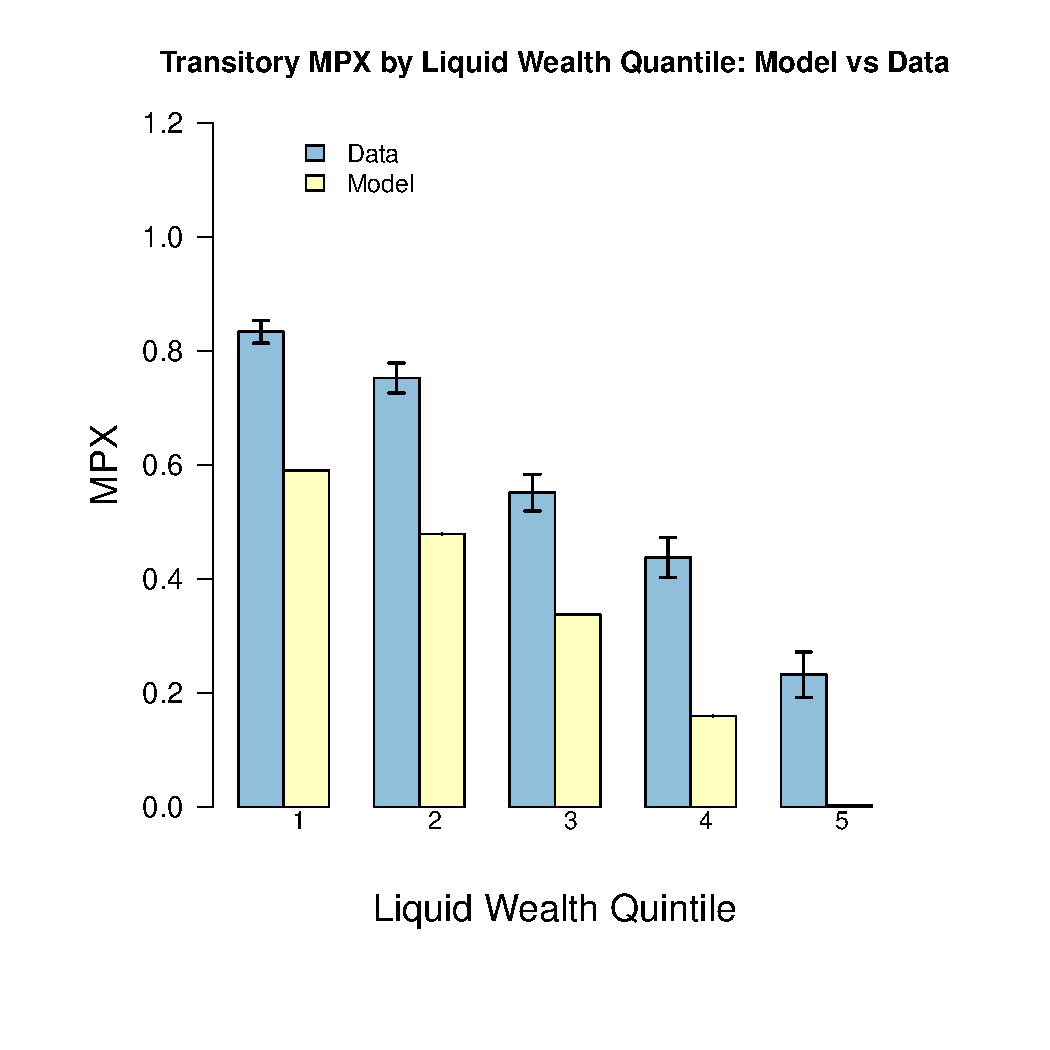
\includegraphics[scale=0.35]{../Figures/CSTW_tran_denmark_pref.pdf}};
	\end{tikzpicture}
\end{columns} 
}
\section{Conclusion}
\frame{
	\frametitle{Conclusion}
	\begin{itemize}
		\item We have designed a new method to estimate consumption responses to income shocks
		\item It appears to work well, both in theory and practice
		\item We can use it to show that heterogeneity plays a key role in monetary policy transmission
	\end{itemize}
	\bigskip
	Thank you!
}
\appendix
\section{MPC vs MPX}
\frame
{
	\frametitle{Durables}
	We have data on value of household cars\\
	\begin{itemize}
		\item Construct expenditure excluding car purchases and sales
		\begin{align*}
		C_T^{\text{nocar}} = C_T - \Delta \text{CarValue}
		\end{align*}
		\item Construct proxy for non durable consumption (Cars $\approx 42.1\%$ durable expenditure)
		\begin{align*}
		C_T^{\text{nondurable}} = C_T - \frac{1}{0.421}\Delta \text{CarValue}
		\end{align*}
	\end{itemize}
}
\frame
{
	\frametitle{Durables}
	\begin{center}
		\begin{tikzpicture}
		\node (img1) {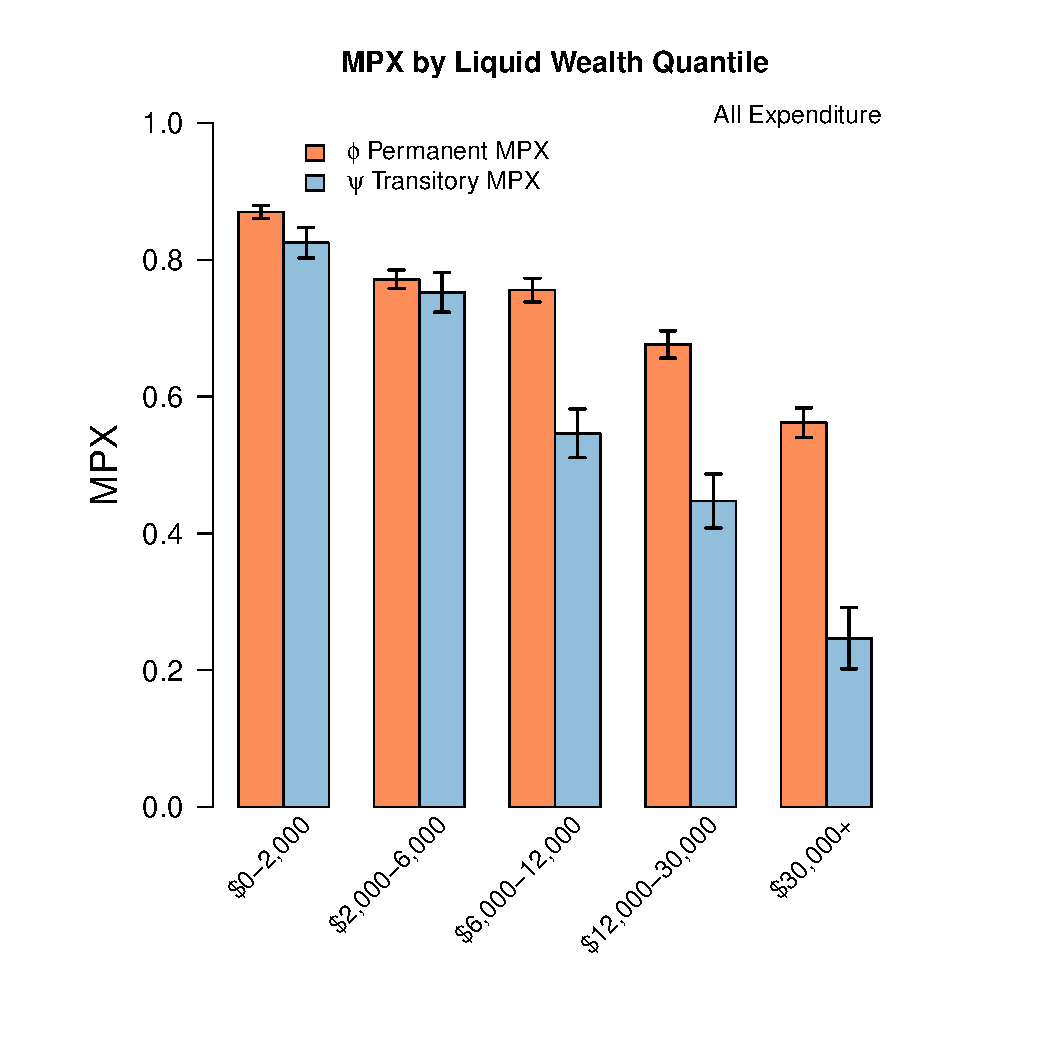
\includegraphics[scale=0.4]{../Figures/MPXByDurables_all.pdf}};
		\pause
		\node (img2)
		{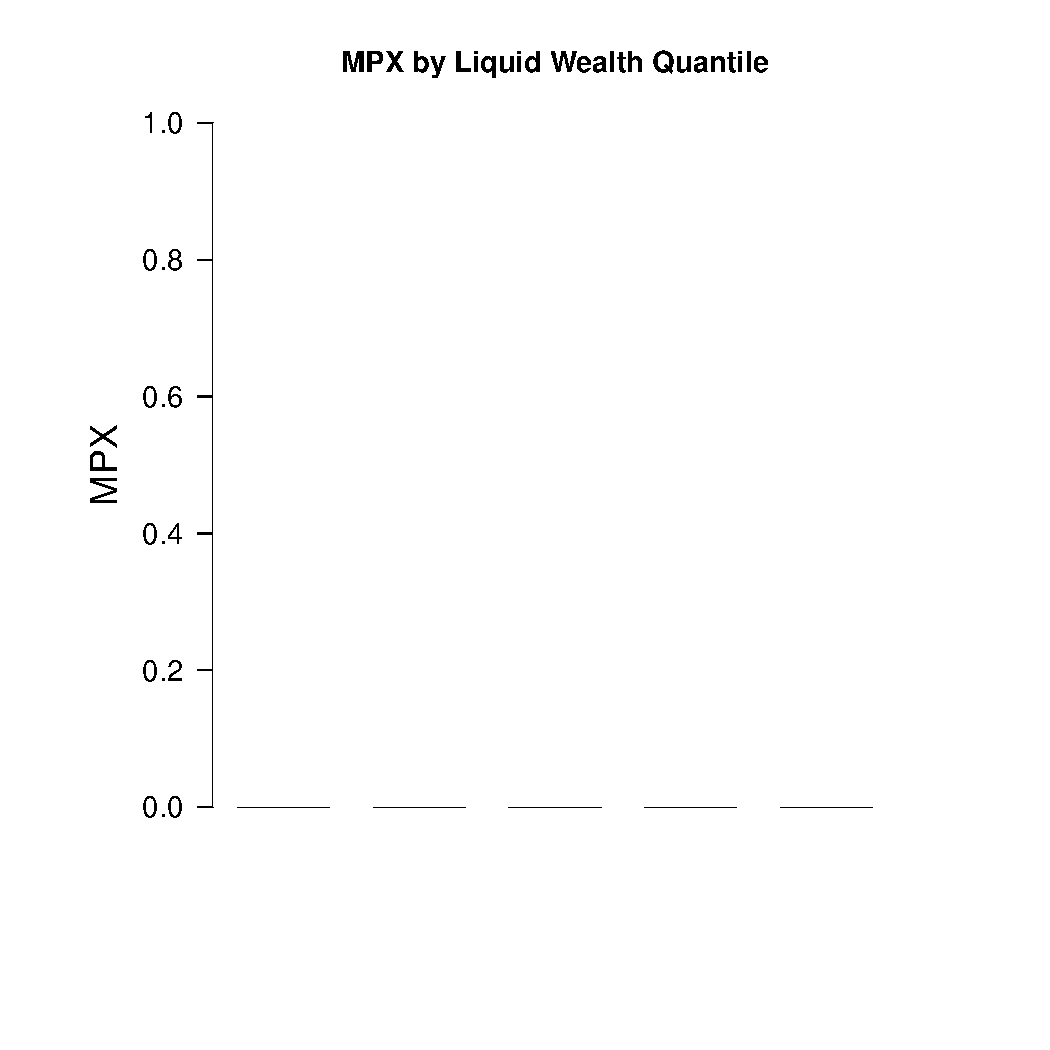
\includegraphics[scale=0.4]{../Figures/MPXByDurables_blank.pdf}};
		\node (img3) {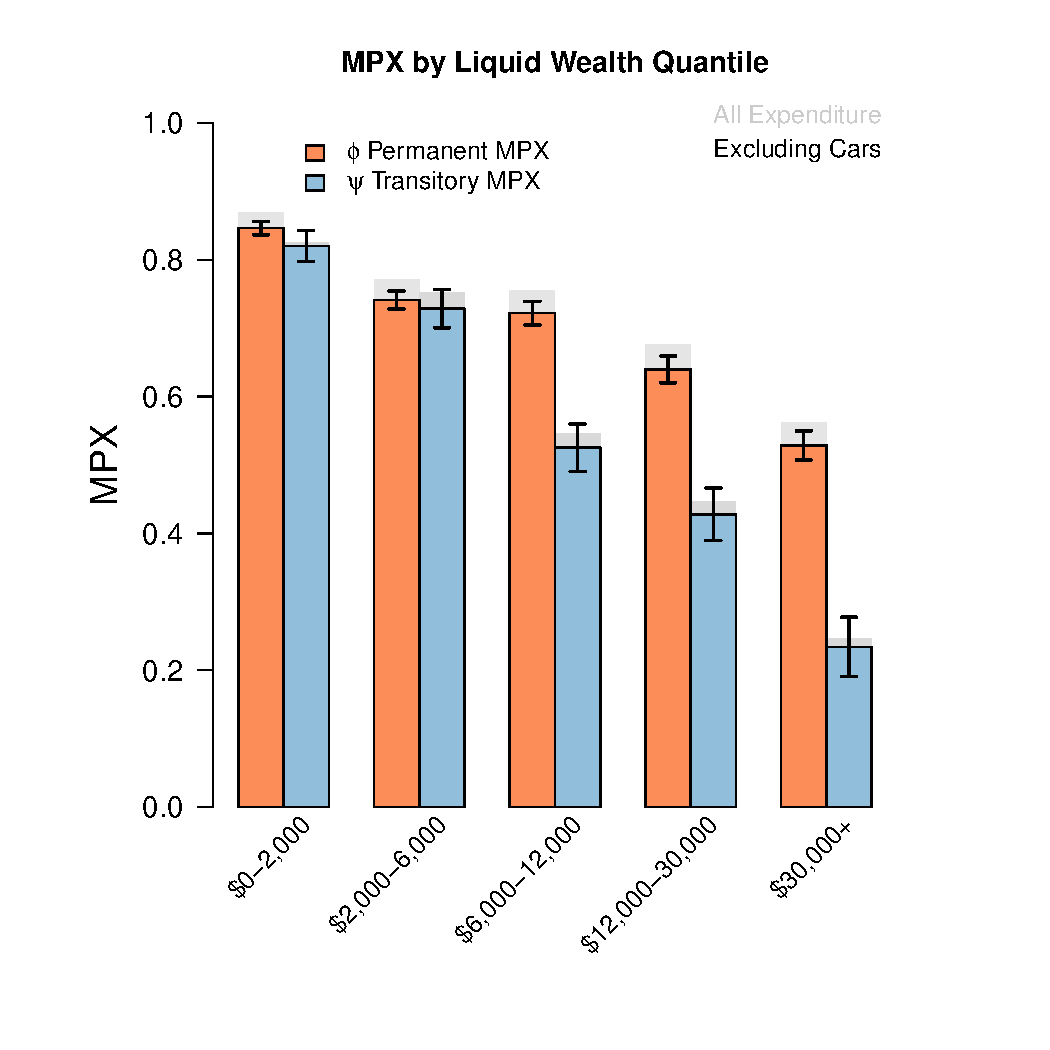
\includegraphics[scale=0.4]{../Figures/MPXByDurables_nocar.pdf}};
		\pause
		\node (img4)
		{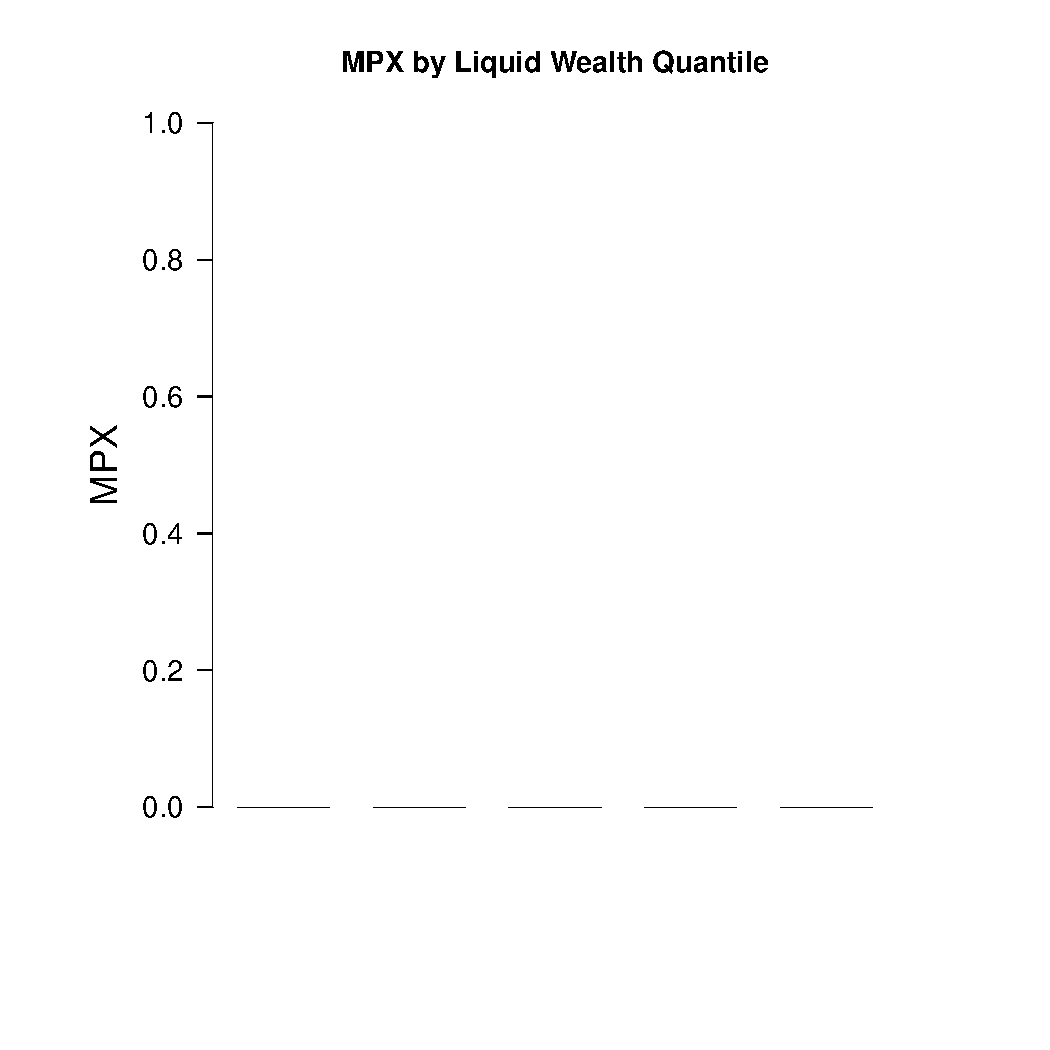
\includegraphics[scale=0.4]{../Figures/MPXByDurables_blank.pdf}};
		\node (img5) {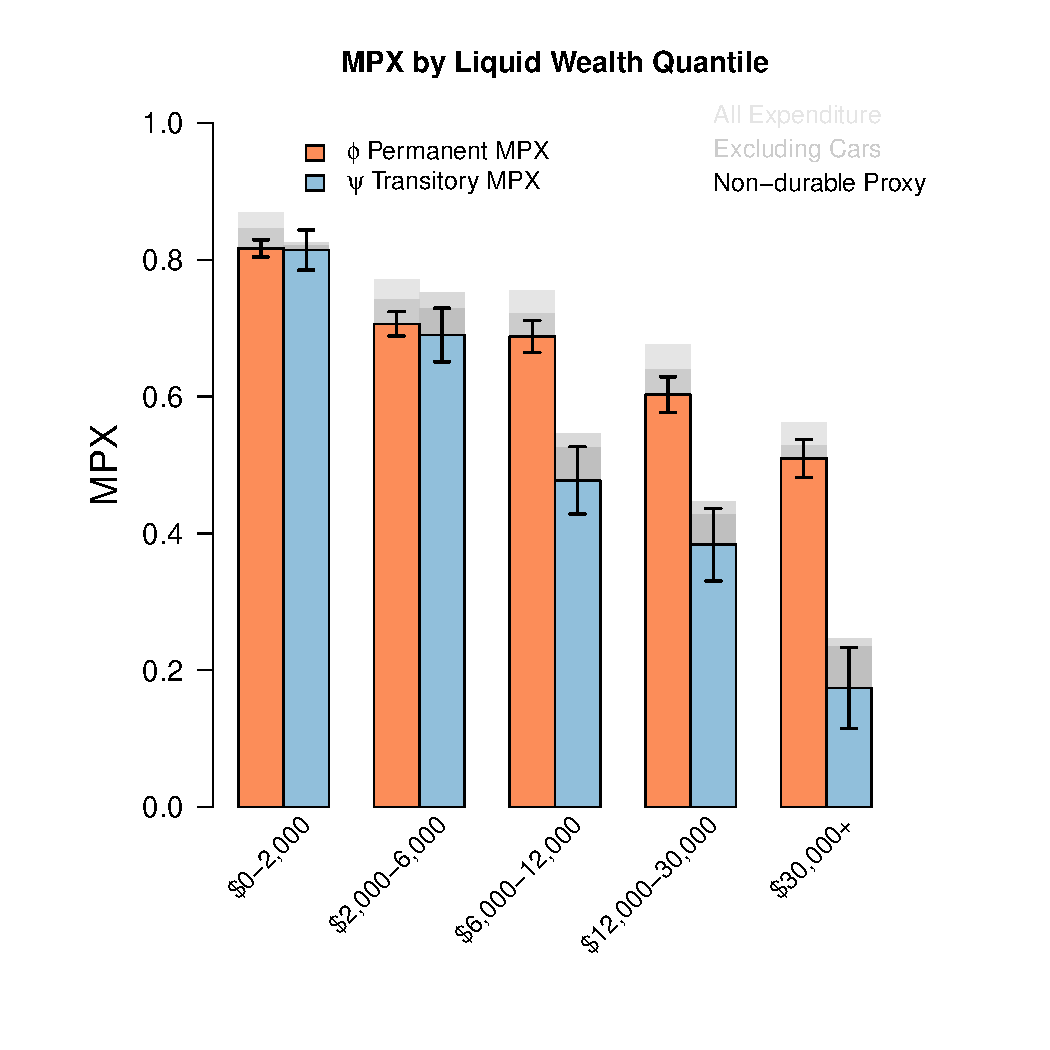
\includegraphics[scale=0.4]{../Figures/MPXByDurables_nodurableproxy.pdf}};
		\end{tikzpicture}
	\end{center}
}
\section{Appendix}
\frame
{
	\frametitle{Methodology Intuition and Suggestive Findings}
	\label{Intuition}
	Exploit increasing importance of permanent shocks as the time over which growth is measured increases
	\begin{columns}
	\column{0.6\linewidth}
	\centering
	\begin{tikzpicture}
	\node (img1) {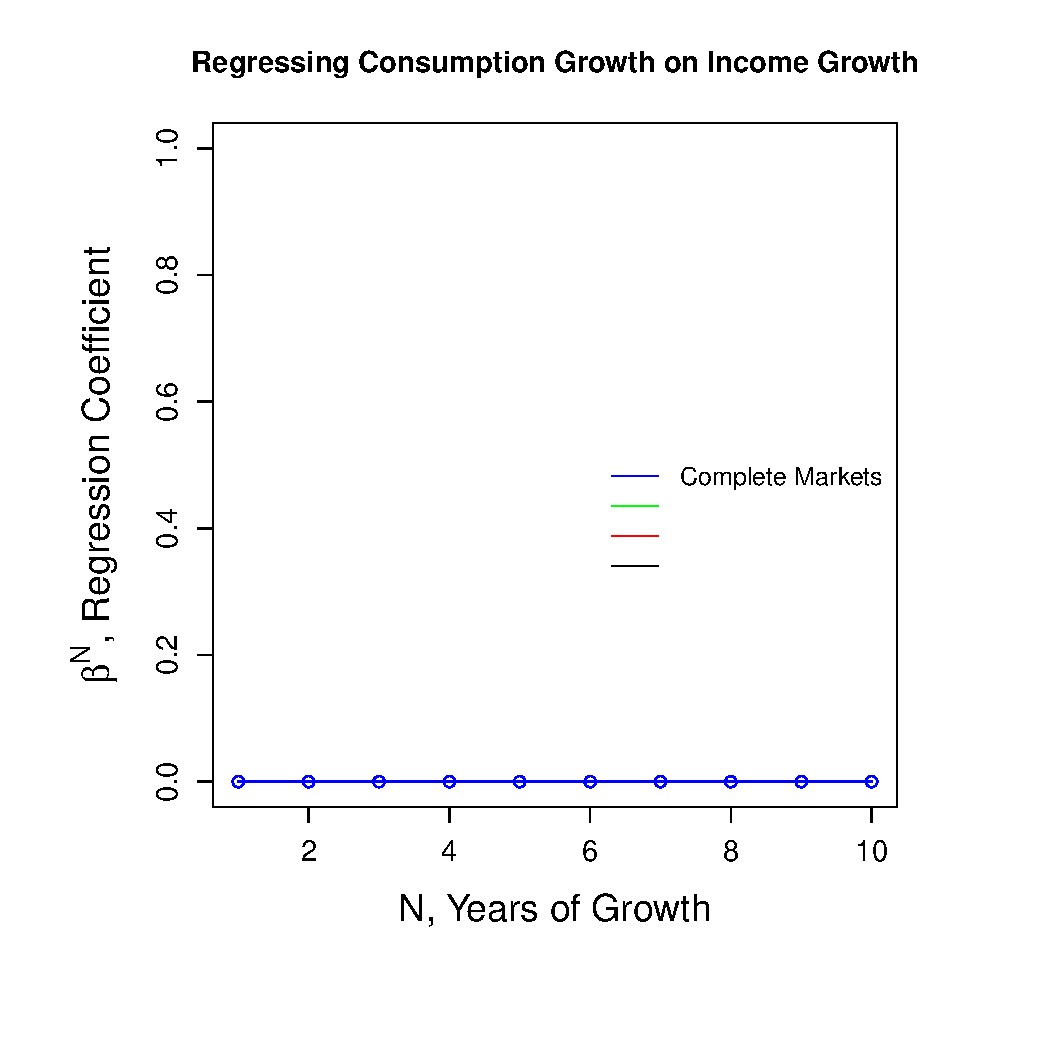
\includegraphics[height=6.5cm]{../Figures/basic_regression_complete_level_lincome_head.pdf}};
	\pause
	\node (img2) {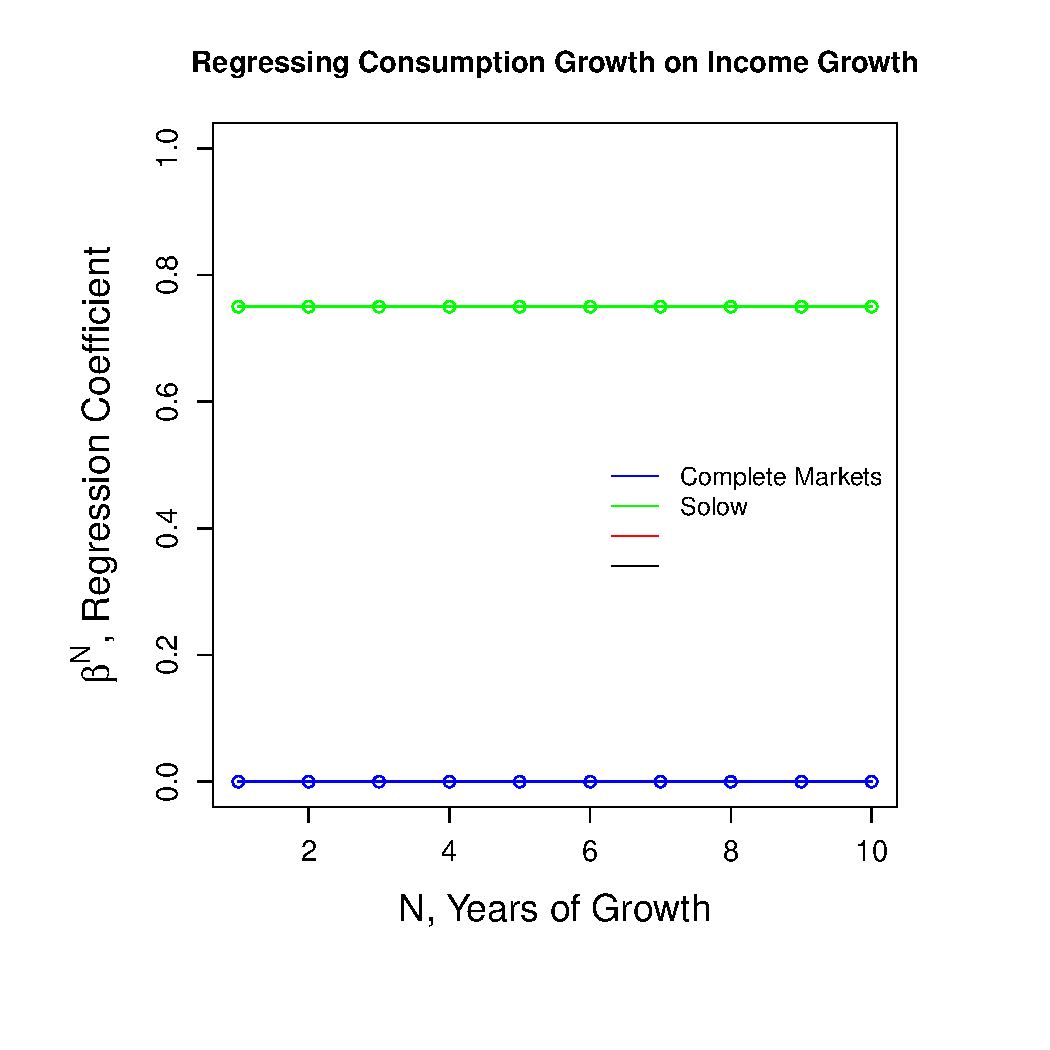
\includegraphics[height=6.5cm]{../Figures/basic_regression_solow_level_lincome_head.pdf}};
	\pause
	\node (img3) {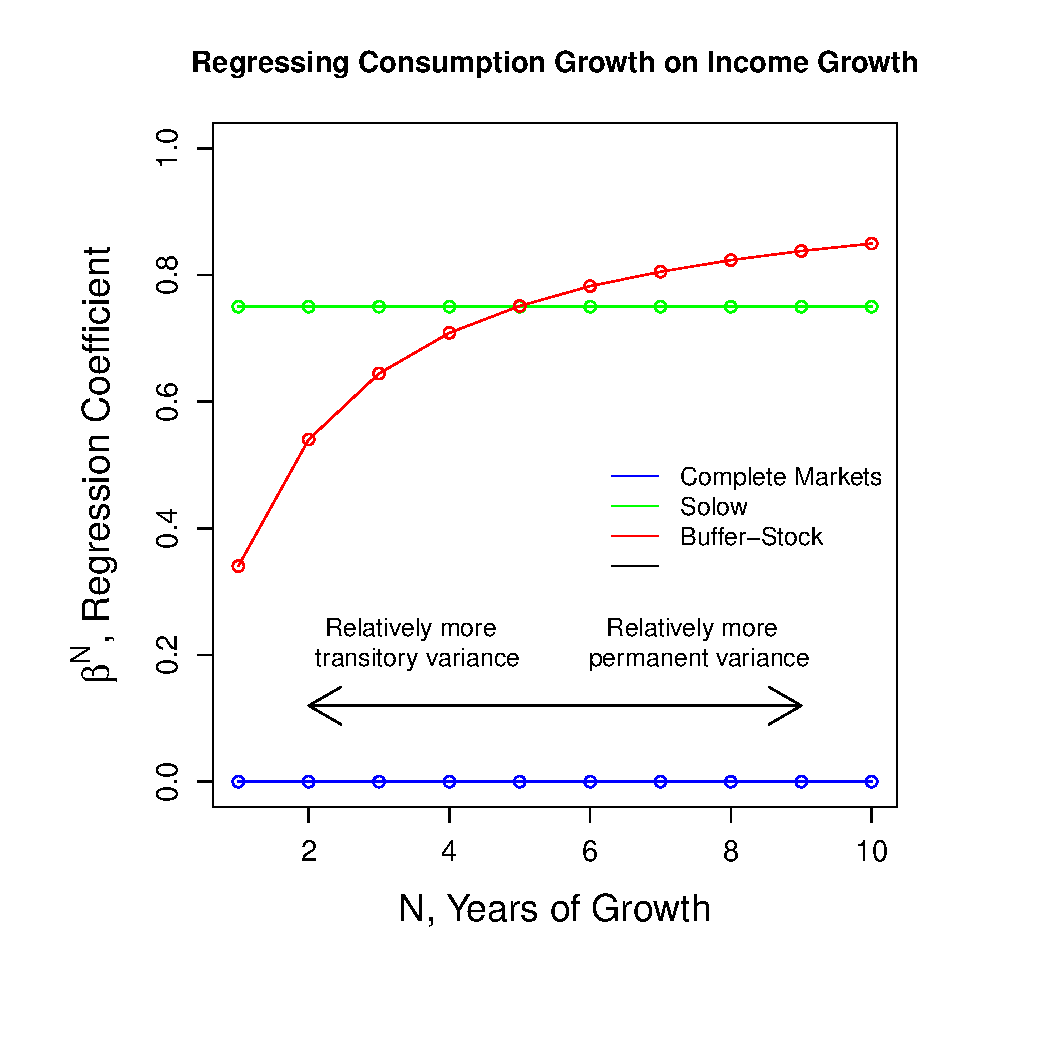
\includegraphics[height=6.5cm]{../Figures/basic_regression_BS_level_lincome_head.pdf}};
	\pause
	\node (img4) {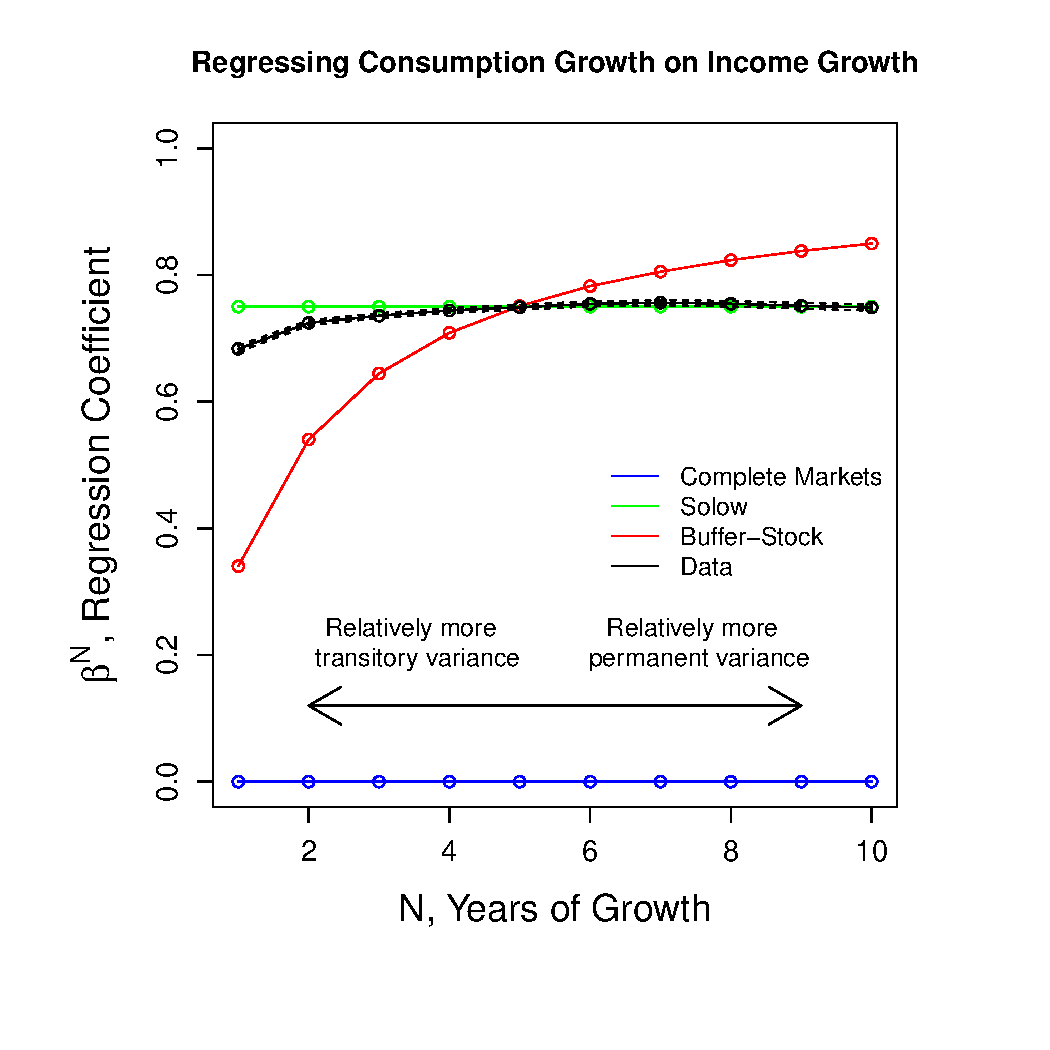
\includegraphics[height=6.5cm]{../Figures/basic_regression_level_lincome_head.pdf}};
	\pause
	\node (img5) {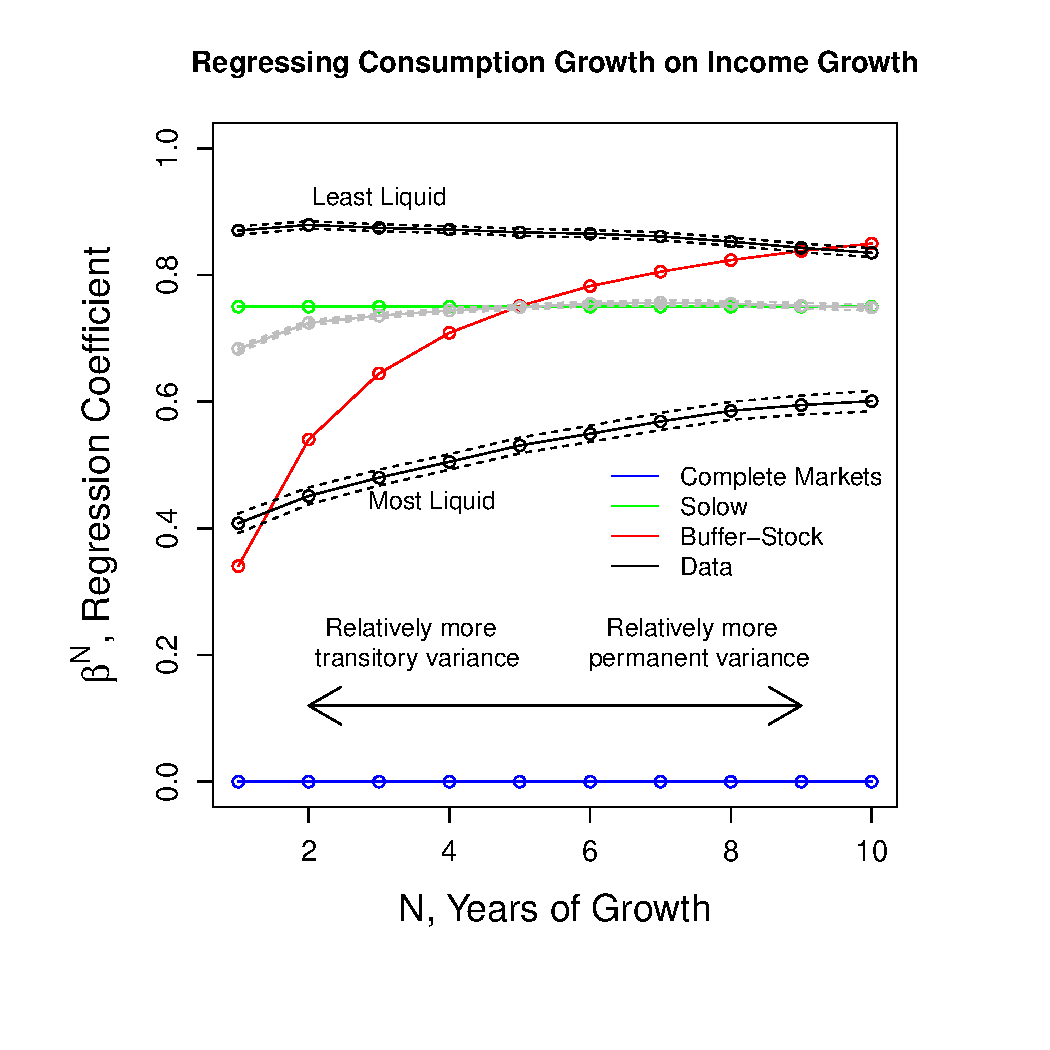
\includegraphics[height=6.5cm]{../Figures/basic_regression_liquid_wealth_level_lincome_head.pdf}};
	\end{tikzpicture}
	\column{0.4\linewidth}
	\begin{align*}
	\Delta^N c_i = \alpha^N + \beta^N \Delta^N y_i +\varepsilon_i
	\end{align*}
	\end{columns}

}
\frame
{
	\frametitle{Aside: Why Not Blundell, Pistaferri and Preston 2008?}
	\label{BPP}
	\textbf{Common Assumptions}\\
	Income $y_t$ is made up of:
	\begin{itemize}
		\item Permanent Income (random walk)
		\item Transitory Income (uncorrelated over time)
	\end{itemize}
	\bigskip
	\textbf{Key to BPP Identification}\\
	$\Delta y_{t+1}$ is a \textit{valid instrument} for transitory shocks in year $t$
	\begin{itemize}
		\item Negatively correlated with transitory shocks in year $t$
		\item U\tikzmark{start}ncorrelated with permanent shocks in year \tikzmark{end}$t$ \\
	\end{itemize}
	\pause
	\bigskip
	Fails due to the \textbf{Time Aggregation Problem}
	
\begin{tikzpicture}[remember picture,overlay]
	\node[draw,line width=2pt,red,ellipse,inner ysep=10pt,fit={(pic cs:start) (pic cs:end)}] {};
	\end{tikzpicture} 
	\hyperlink{Time_aggregation}{\beamerbutton{Time aggregation problem}}
}
\frame
{
	\frametitle{Time Aggregation Problem (Crawley 2018)}
	\label{time_aggregation}
	\begin{columns}
	\column{0.5\linewidth}
	\centering
	\onslide<1->{
	\begin{tikzpicture}
	\node (img1) {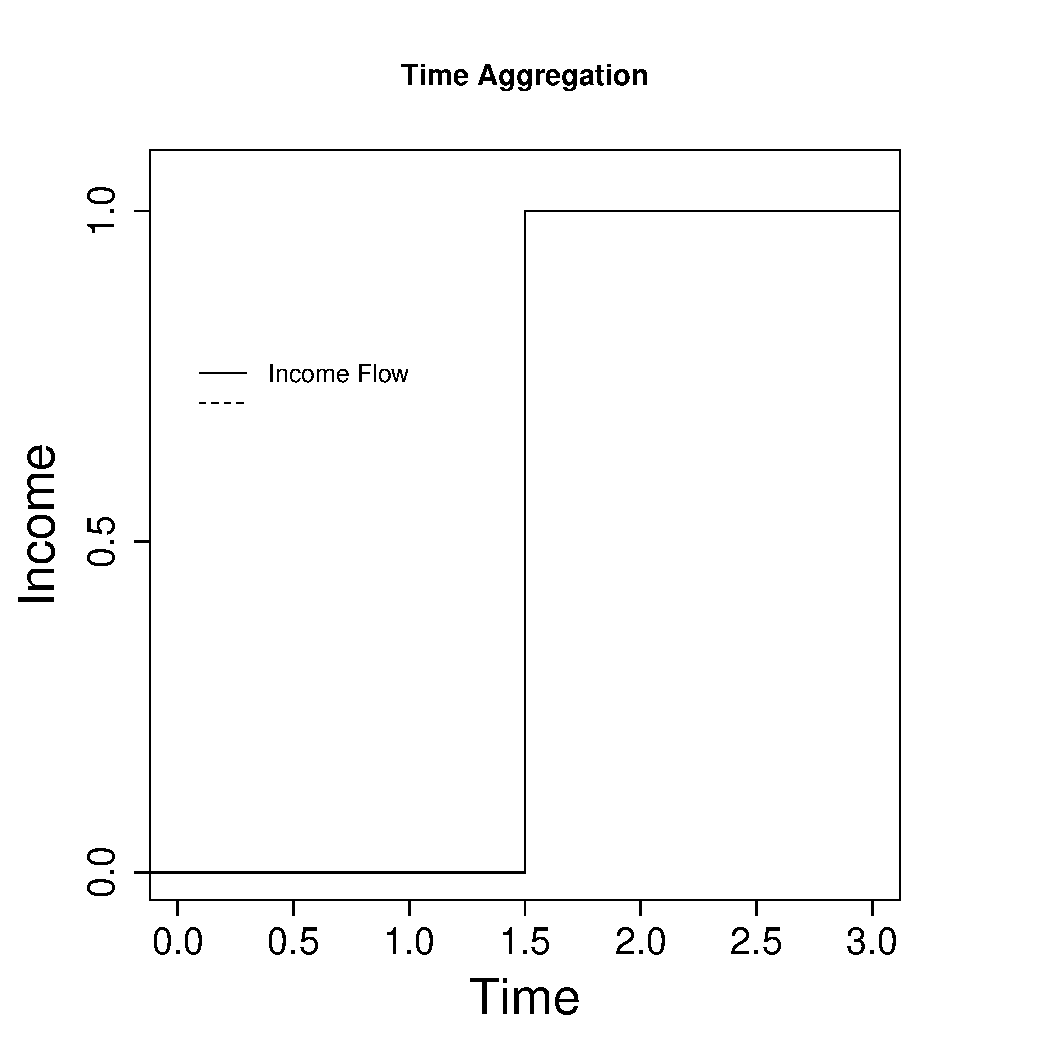
\includegraphics[height=5cm]{../Figures/TimeAggExample1.pdf}};
	\onslide<2->{
	\node (img2) {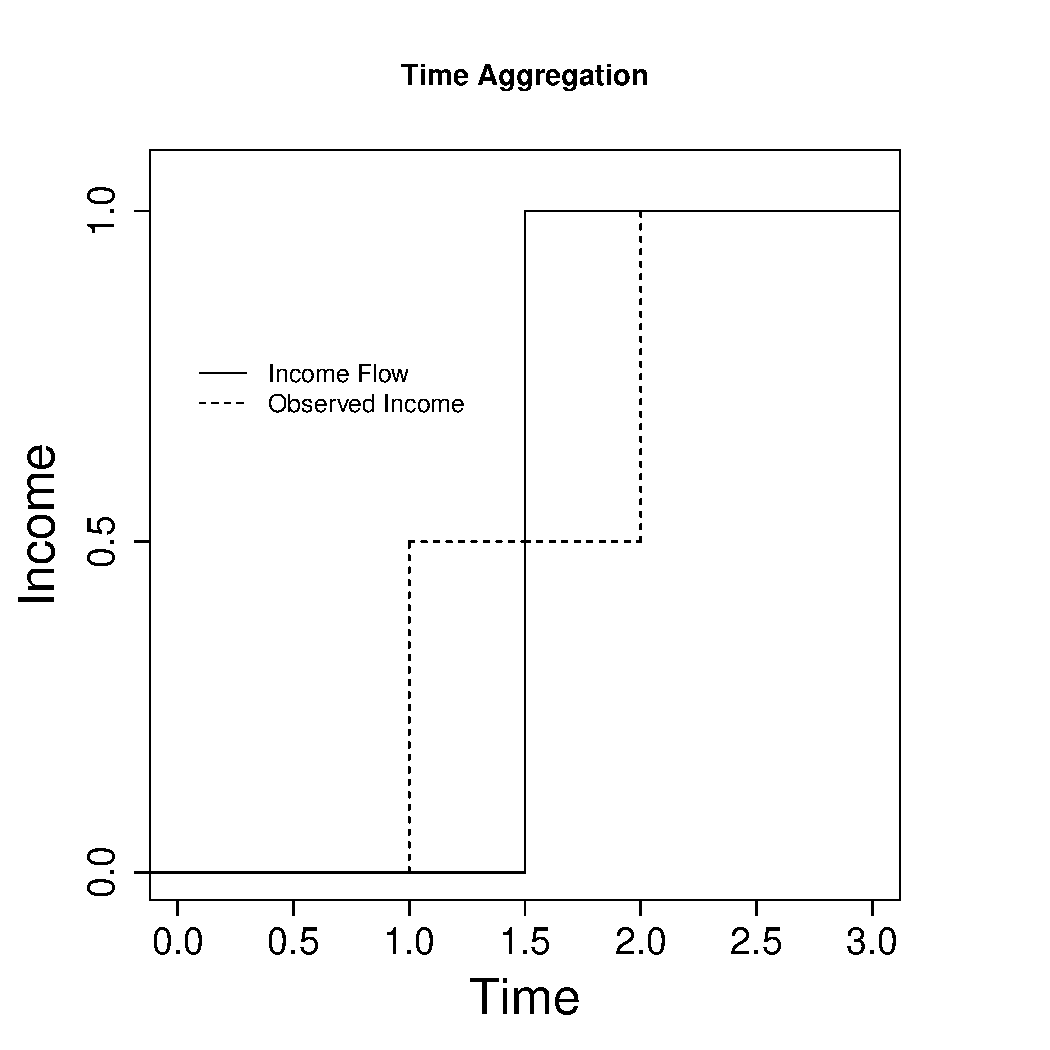
\includegraphics[height=5cm]{../Figures/TimeAggExample2.pdf}};
	}
	\end{tikzpicture}
	}
	\column{0.5\linewidth}
	\onslide<3->{Observed permanent income growth is \textit{positively} autocorrelated\\
	\bigskip
	BPP misinterprets \textit{positive} permanent income shocks as \textit{negative} transitory shocks\\
	\bigskip
	$\implies$ Thinks negative transitory shocks result in consumption \textit{increasing}
	\end{columns}
	}
	\onslide<4->{If the Permanent Income Hypothesis holds, BPP will estimate the MPC to be -0.6}
}

\frame
{
	\frametitle{Identification Restrictions: Income}
	\label{Income_process}
	Income flow consists of:
	\begin{itemize} 
		\item Permanent Income (random walk)
		\item Transitory Income (persistence $<$ 2 years)
	\end{itemize}
	\begin{figure}
		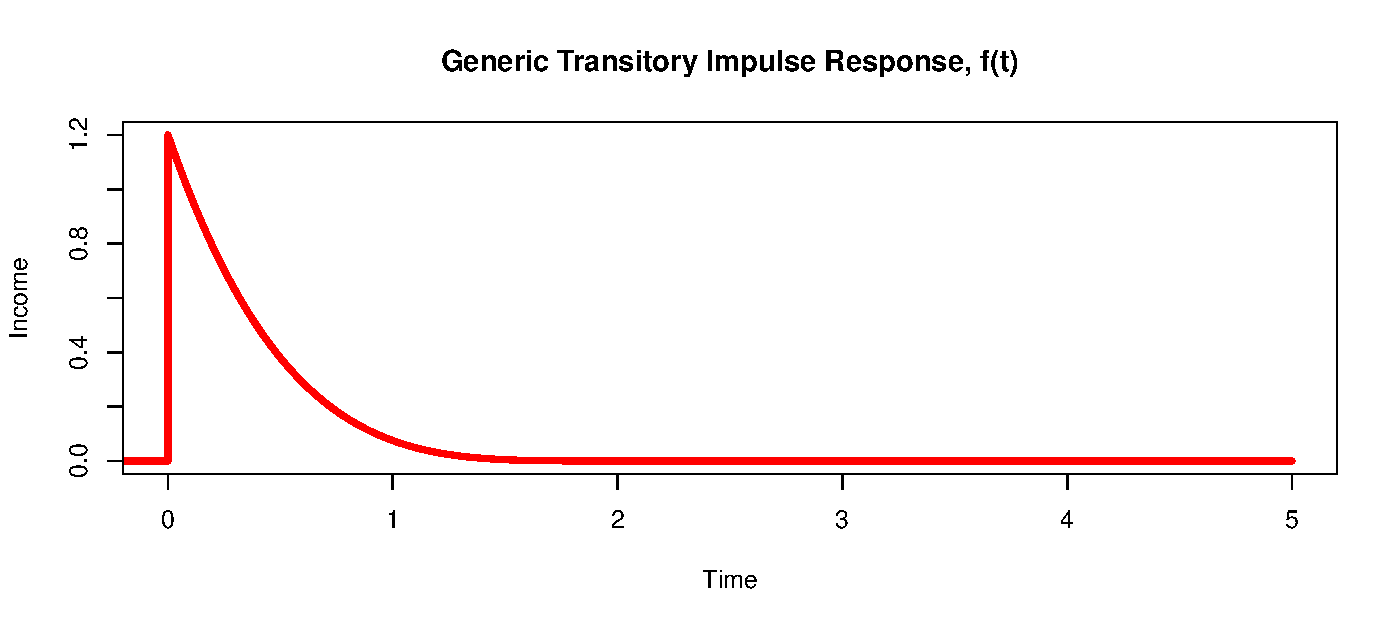
\includegraphics[scale=0.35,trim= 0 2.5cm 0 1cm]{../Figures/GenericTransitory.pdf}
	\end{figure}
	\begin{align*}
	\onslide<2->{\color{red} \tikz[baseline]{\node(n1){}}\bar{y}_T =} \onslide<2->{\tikz[baseline]{\node(n2){}}\int_{T-1}^{T}}\color{black} y_t\onslide<2->{\color{red}dt} &= \onslide<2->{ \color{red} \int_{T-1}^{T}}\color{black} \tikz[baseline]{\node(n4){}}p_t \onslide<2->{\color{red}dt} \color{black} + \onslide<2->{\color{red}\int_{T-1}^{T}}\color{black}\int_{t-2}^{t} \tikz[baseline]{\node(n5){}}f(t-s)dq_s\onslide<2->{\color{red}dt}
	\end{align*}
	\only<1>{
	\begin{tikzpicture}[remember picture,overlay]
	\node (n4a)  at ([shift={(0.2,-0.05)}]n4) {};
	\node (n5a)  at ([shift={(0.5,-0.2)}]n5) {};
	\draw[blue,thick,->] (n4a)  to [in=90,out=245] + (225:1.3cm) node[anchor=north,text = blue] {Permanent income flow};
	\draw[blue,thick,->] (n5a) to [in=90,out=245] + (290:0.8cm) node[anchor=north,text = blue] {Transitory income flow};
	\end{tikzpicture}
	}
	\only<2>{
	\begin{tikzpicture}[remember picture,overlay]
	\node (n1a)  at ([shift={(0.25,0.2)}]n1) {};
	\node (n2a)  at ([shift={(0.45,-0.45)}]n2) {};
	\draw[blue,thick,->] (n1a)  to [in=270,out=90] + (90:0.6cm) node[anchor=south,text = blue] {Observed Income};
	\draw[blue,thick,->] (n2a)  to [in=90,out=270] + (270:0.6cm) node[anchor=north,text = blue] {Time Aggregation};
	\end{tikzpicture}
	}
}
\frame
{
	\frametitle{Identification Restrictions: Income}
	
	\begin{align*}
	\only<1->{\bar{y}_T  &= \int_{T-1}^{T} p_t dt + \int_{T-1}^{T} \int_{t-2}^{t} f(t-s)dq_s dt \\[7pt]
		\Delta^N \bar{y}_T &= \bar{y}_T - \bar{y}_{T-N} \\
		                   &= \int_{T-1}^{T} (p_t-p_{T-1})dt \tikz[baseline]{\node(d1){}} - \int_{T-N-1}^{T-N} (p_t-p_{T-N})dt \tikz[baseline]{\node(d2){}}\\ 
		& \qquad   + (p_{T-1}-p_{T-N}) \tikz[baseline]{\node(d3){}}\\
		& + \int_{T-1}^{T} \int_{t-2}^{t} f(t-s)dq_s dt \tikz[baseline]{\node(d4){}} - \int_{T-N-1}^{T-N} \int_{t-2}^{t} f(t-s)dq_s dt \tikz[baseline]{\node(d5){}} }
	\end{align*}
	\vspace{1cm}
		\begin{align*}
		\only<3->{\implies \mathrm{Var}(\Delta^N \bar{y}_T) &= (N-\frac{1}{3})\sigma^2_p +  2 \sigma^2_{\tilde{q}} \text{   for }N \geq 3 }
		\end{align*}
	\only<1->{
	\begin{tikzpicture}[remember picture,overlay]
	\node (d1a)  at ([shift={(-1.0,-0.1)}]d1) {};
	\node (d2a)  at ([shift={(-2.0,-0.1)}]d2) {};
	\node (d3a)  at ([shift={(2.9,0.1)}]d3) {};
	\node (d4a)  at ([shift={(-2.1,-0.2)}]d4) {};
	\node (d5a)  at ([shift={(-2.1,-0.2)}]d5) {};
	\node (d6)  at ([shift={(0.3,-1.0)}]d4) {};
	\draw[blue,thick,->] (d1a)  to [in=180,out=330] (d3a) node[anchor=north,text = black] {};
	\draw[blue,thick,->] (d2a)  to [in=180,out=245] (d3a) node[anchor=north,text = black] {};
	\draw[blue,thick,->] (d3)   to [in=180,out=0  ] (d3a) node[anchor=west,text = blue, text width=3.5cm,font=\small] {Independent increments $\mathrm{Var} = (\frac{1}{3}+\frac{1}{3}+N-1)\sigma^2_p$};
	\end{tikzpicture}
	}
	\only<2->{
	\begin{tikzpicture}[remember picture,overlay]
	\draw[blue,thick,->] (d4a)  to [in=150,out=330] (d6) node[anchor=north,text = black] {};
	\draw[blue,thick,->] (d5a)  to [in=30,out=245] (d6) node[anchor=north,text = blue,font=\small] {Independent if $N\geq 3$};
	\end{tikzpicture}
	}	
}
\frame
{
	\frametitle{Identification Restrictions: Consumption}
	\label{cons_identification}
	Assumptions on Consumption\\
	\begin{itemize}
		\item Permanent: Consumption permanently moves by fraction $\phi$ of the income shock
		\item Transitory: Persistence $<$ 2 years \qquad \qquad \qquad \qquad \hyperlink{cons_decay}{\beamerbutton{Evidence}}
	\end{itemize}
	\vspace*{-0.2in}
	\begin{center}
	\begin{tikzpicture}
	\node (img1) {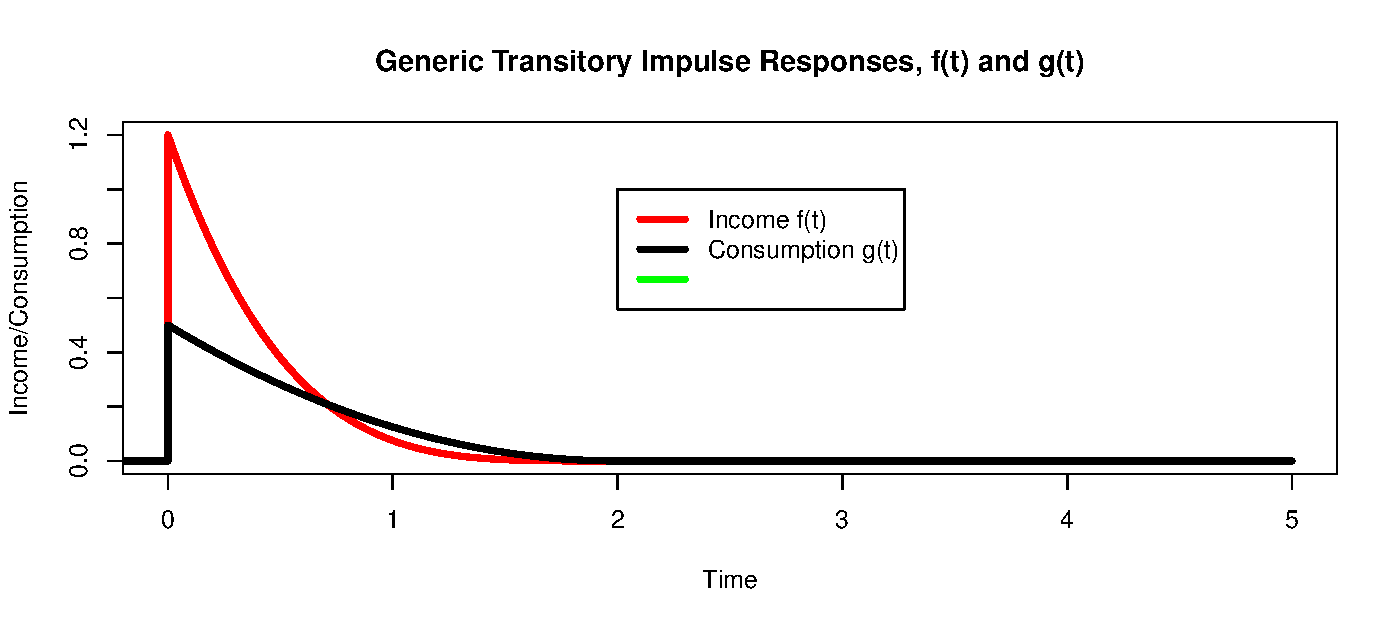
\includegraphics[height=3.5cm]{../Figures/GenericTransitoryConsumption.pdf}};
	\pause
	\node (img2) at (img1) {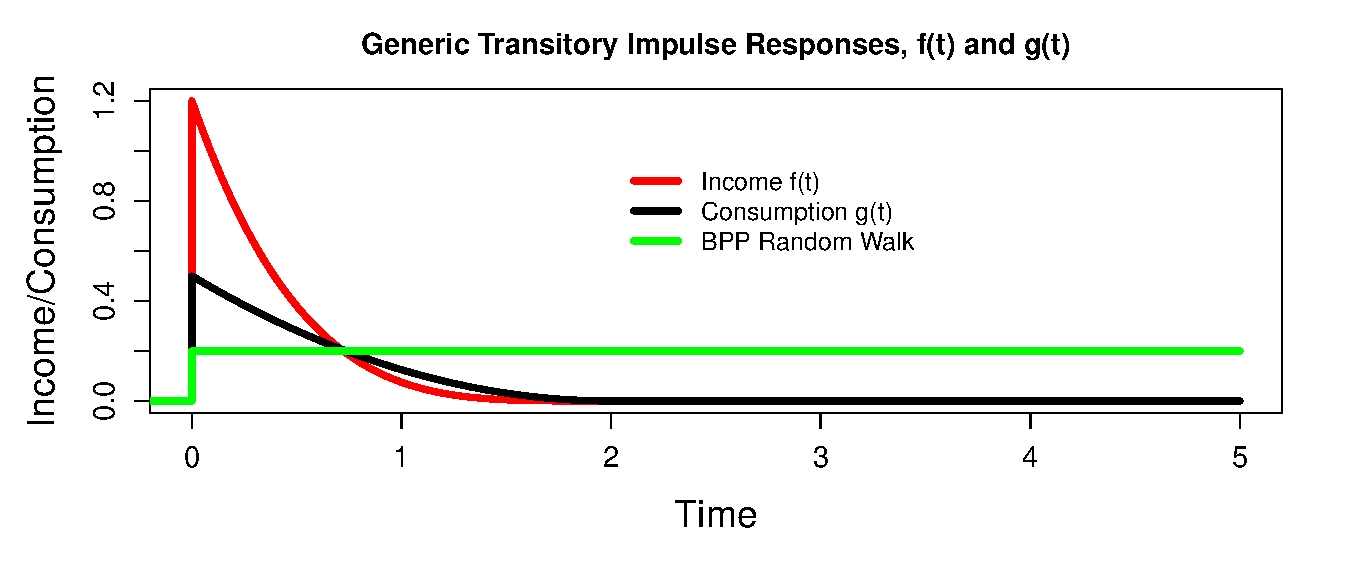
\includegraphics[height=3.5cm]{../Figures/GenericTransitoryConsumptionWithBPP.pdf}};
	\node (text)  at ([shift={(-1,-2.0)}]img1) {This is a key difference between what we assume and BPP};
	\end{tikzpicture}
	\end{center}
}
\frame
{
	\frametitle{Identification Restrictions: Consumption}
	Consumption flow is given by:
	\begin{align*}
	c_t  &= \phi p_t  + \int_{t-2}^{t} g(t-s)dq_s  \\
	\implies \mathrm{Cov}&(\Delta^N \bar{c_T},\Delta^N \bar{y_T} ) = \phi (N-\frac{1}{3}) \sigma^2_p + 2 \psi \sigma^2_{\tilde{q}}
	\end{align*}
	where  $\psi = \frac{\mathrm{Cov}(\tilde{c},\tilde{q})}{\mathrm{Var}(\tilde{q})}$, the regression coefficient of `transitory' consumption on transitory income \\
	\pause
	\bigskip
	\begin{itemize}
		\item $\phi$: MPX out of permanent income shocks
		\item $\psi$: MPX out of transitory income shocks
	\end{itemize}
	\textbf{M}arginal \textbf{P}ropensity to e\textbf{X}pend (includes durables)
}
\frame{
	\frametitle{Evidence of Consumption Decay Within 2 Years}
	\label{cons_decay}
	\begin{columns}
	\column{0.35\linewidth}
	\begin{figure}
	From \cite{fagereng_mpc_2016}
	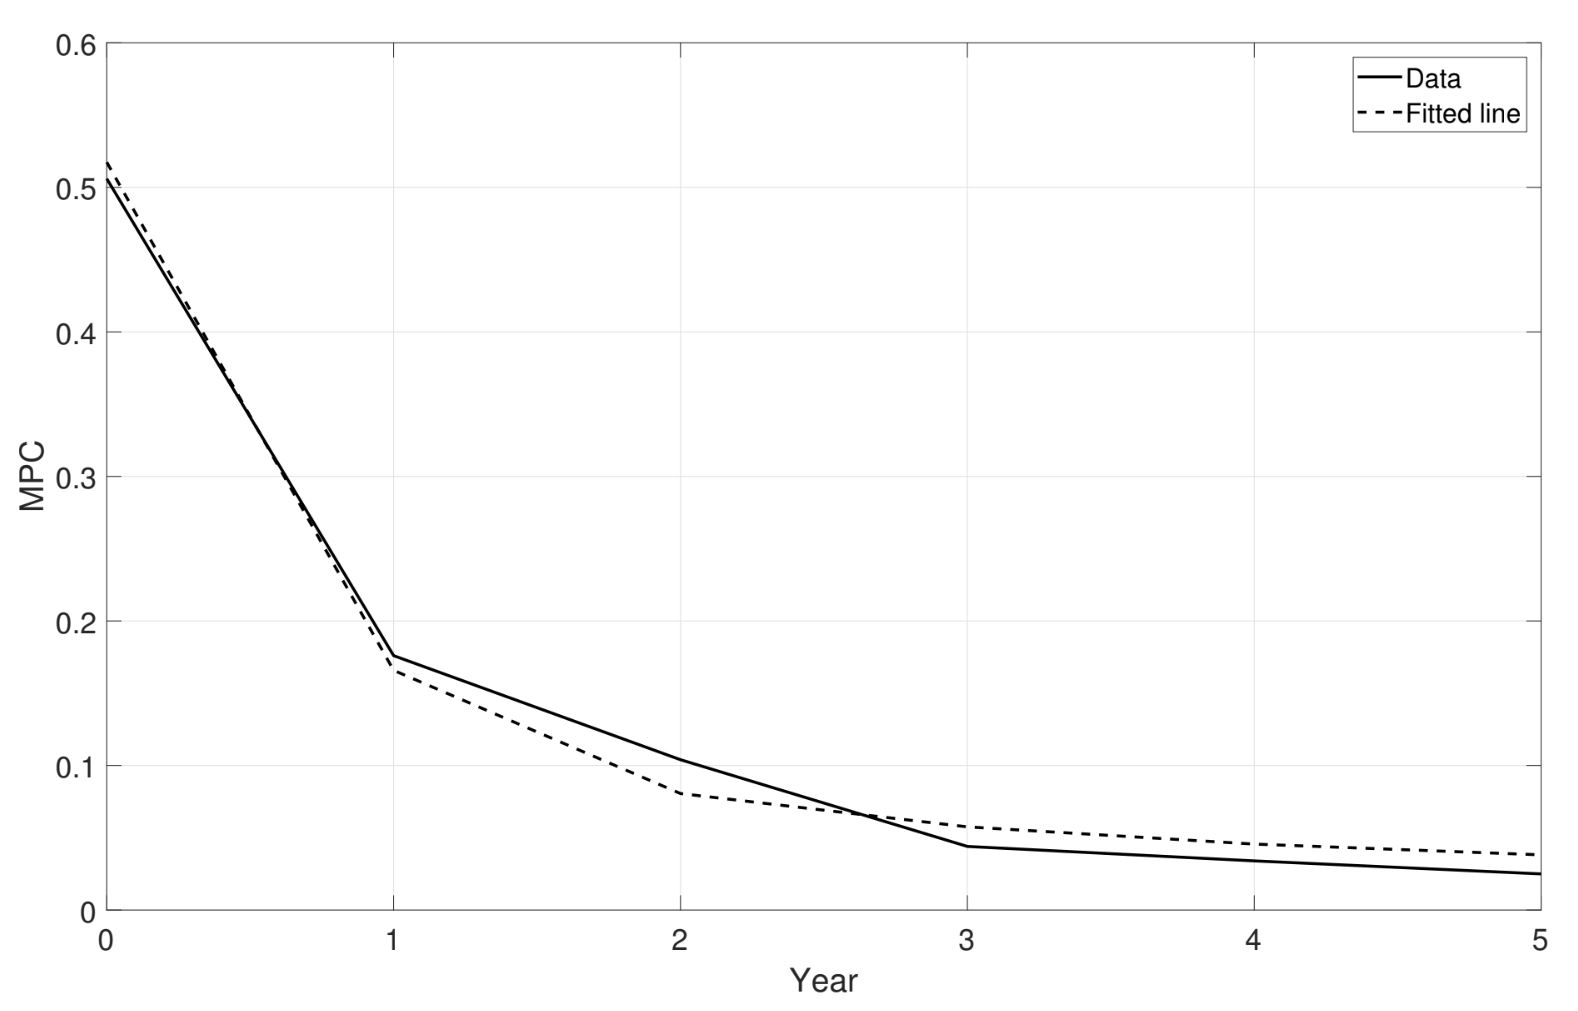
\includegraphics[scale=0.3]{../Figures/norway_cons_decay.JPG}
	\end{figure}
	\column{0.5\linewidth}
	\begin{figure}
	From \cite{gelman_what_2016}
	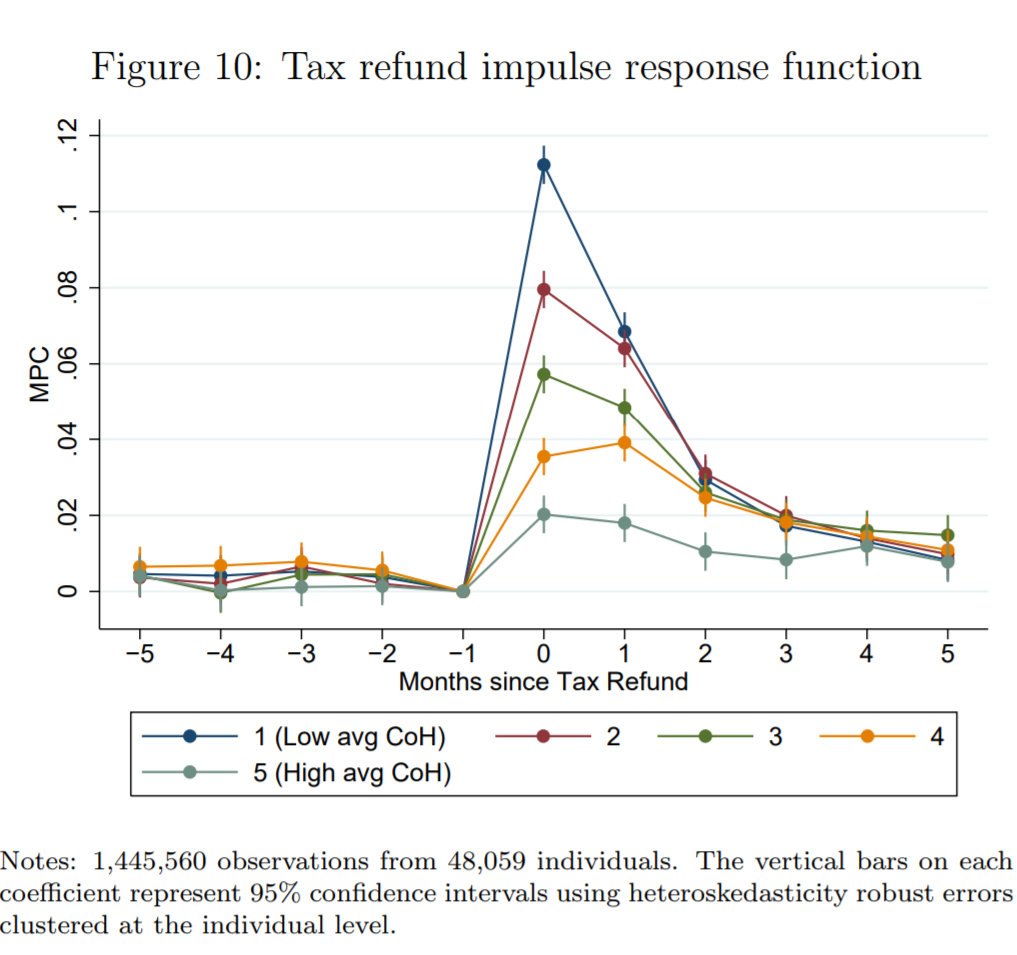
\includegraphics[scale=0.1]{../Figures/gelman_cons_decay.png}
	\end{figure}
	\end{columns}
	\hyperlink{cons_identification}{\beamerbutton{Back}}
}
\frame
{
	\frametitle{Data: When is Measurement Error a Problem?}
	\label{measurement_error}
	Our method has the same measurement error issues as the regressions:
	\begin{align*}
	\Delta^N c_i = \alpha^N + \beta^N \Delta^N y_i +\varepsilon_i
	\end{align*}
	That is:
	\begin{itemize}
		\item[1] Measurement error in $\Delta^N y_i$ leads to attenuation bias
		\item[2] Measurement error in $\Delta^N c_i$ should be uncorrelated with $\Delta^N y_i$
	\end{itemize}
	\bigskip
	When might 2 fail?
	\begin{itemize}
		\item When a proportion of assets are held off balance sheet
		\item When returns are correlated with \textit{changes} in income (e.g. own stock in the company you work for)
		\item When insurance is provided by friends and family
	\end{itemize}
}
\frame
{
	\frametitle{MPX by Net Wealth}
	\label{MPXbyNetWealth}
	\begin{columns}
		\column{0.5\linewidth}
		\centering
		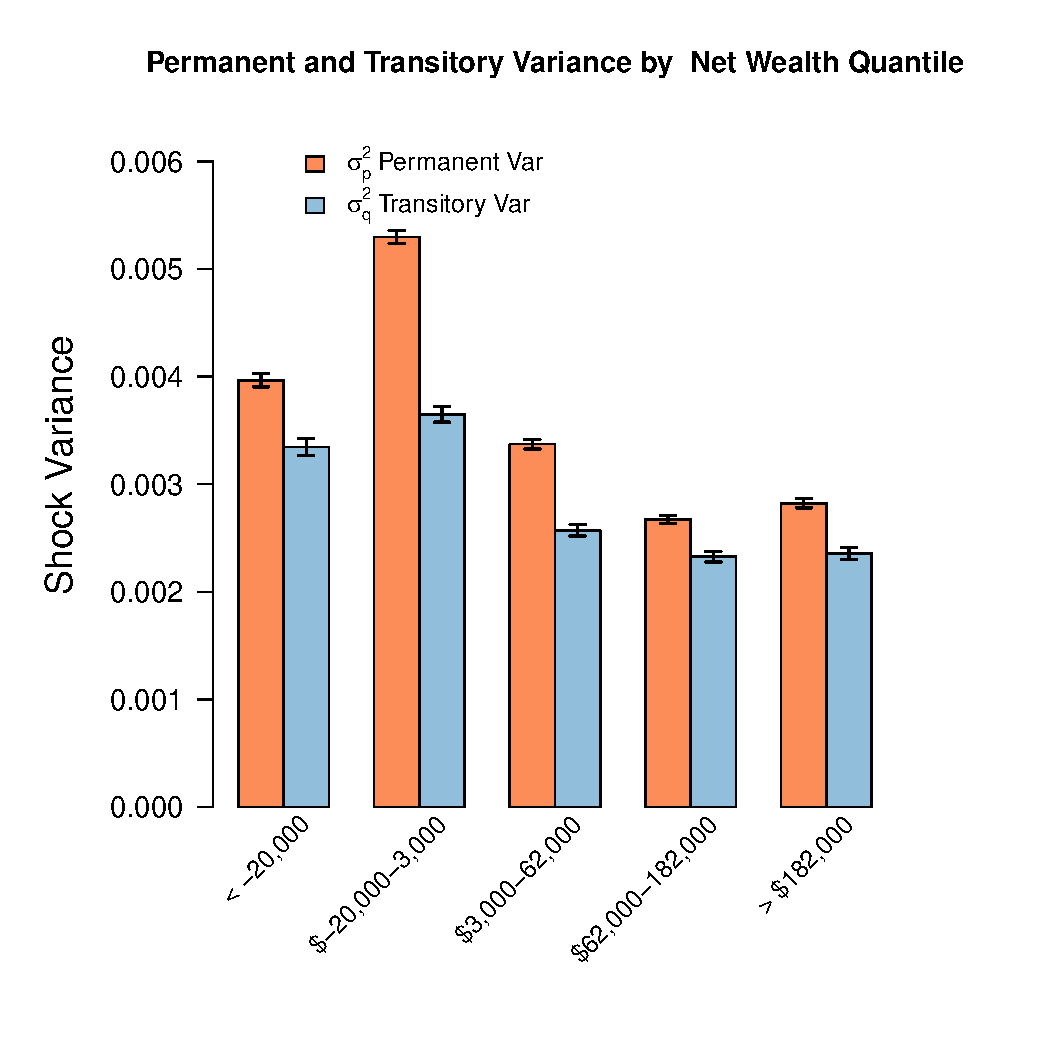
\includegraphics[scale=0.35]{../Figures/VarianceByNetWealth_level_lincome_head.pdf}
		\column{0.5\linewidth}
		\centering
		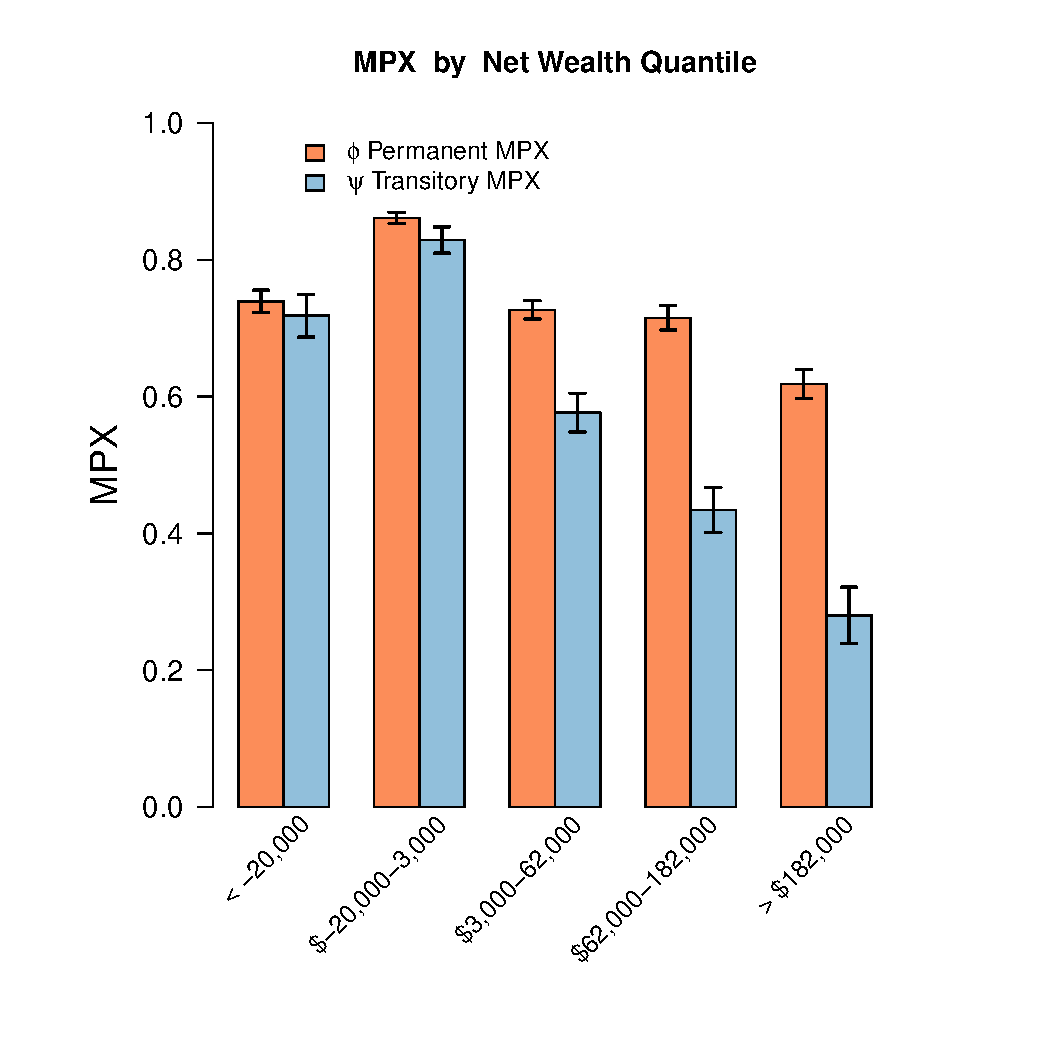
\includegraphics[scale=0.35]{../Figures/MPXByNetWealth_level_lincome_head.pdf}
	\end{columns} 	
	\hyperlink{MPXbyLiquidWealth}{\beamerbutton{Back}}
}
\begin{comment}
\section{Model}
\frame
{
	\frametitle{Model}
	How does this compare with a standard buffer-stock saving model?
	\begin{itemize}
		\item Build model to match Danish income process
		\item Allow \textit{heterogeneous discount factors} in order to match the distribution of \textit{liquid} assets in Denmark
		\item See how the distribution of transitory MPX varies with liquid asset holdings
	\end{itemize}
}
\frame
{
	\frametitle{Model}
Given market resources ($\boldmath{\mLevBF}_t$), households in this model maximize expected utility:
\begin{align*}
\mathbb{E}_t \sum_{i=t}^{\infty} \beta^i(1-D)^i  u(\cLevBF_i)
\end{align*}
subject to the constraints:
\begin{align*}
\aLevBF_t = \mLevBF_t - \cLevBF_t \\
\bLevBF_t = R\aLevBF_t \\
\yLevBF_t = \theta_t \pLevBF_t \\
\pLevBF_t = \Psi_t \pLevBF_{t-1} \\
\mLevBF_t = \bLevBF_t + \yLevBF_t
\end{align*}
}
\frame
{
	\frametitle{Calibration}
	\input ../Tables/CalibrationTable.tex
}
\frame
{
	\frametitle{Lorenz Curve}
	Lorenz Curve for Liquid Wealth Holdings
	\centering
	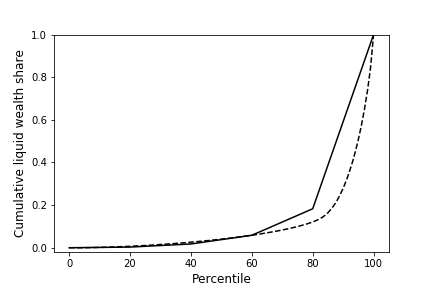
\includegraphics[scale=0.5]{../Figures/Lorenz.png}
}
\frame
{
	\frametitle{Does our Methodology Work?}
	\begin{columns}
	\column{0.5\linewidth}
	\centering
	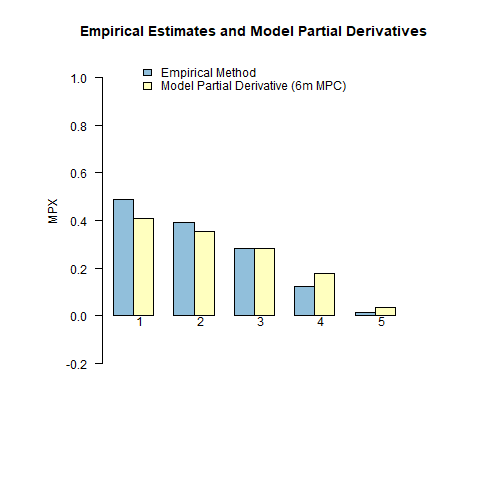
\includegraphics[scale=0.35]{../Figures/MPC_accuracy.png}
	\column{0.5\linewidth}
	\begin{itemize}
		\item Estimate is larger than 6m MPX for low liquid wealth
		\begin{itemize}
		\item Income jumps can be large
		\end{itemize}
		\item Estimate is smaller than 6m MPX for high levels of wealth
		\begin{itemize}
		\item Consumption response lasts more than 2 years
		\end{itemize}
	\end{itemize}
	\end{columns}
}
\frame
{
	\frametitle{Model vs Data}
	How does the model compare with the data?
	\begin{columns}
	\column{0.5\linewidth}
	\centering
	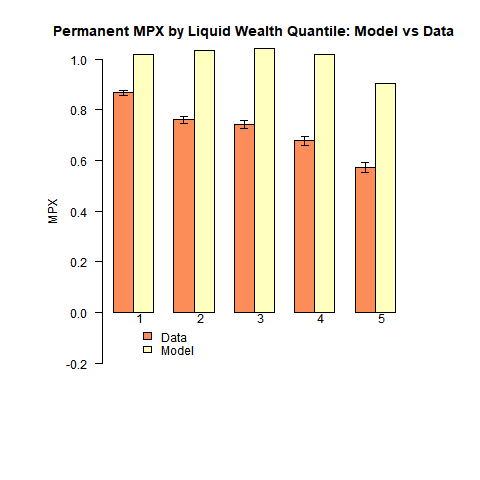
\includegraphics[scale=0.35]{../Figures/CSTW_perm_denmark.png}
	\column{0.5\linewidth}
	\centering
	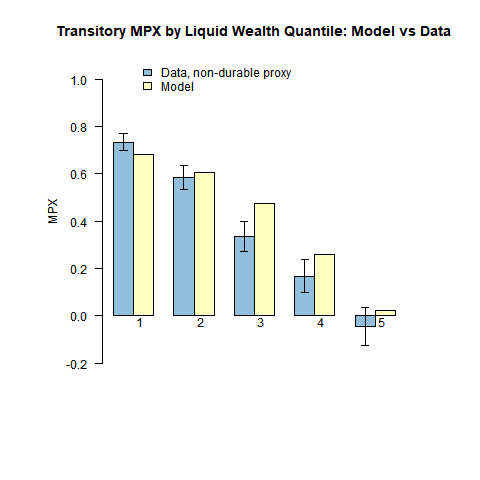
\includegraphics[scale=0.35]{../Figures/CSTW_tran_denmark.png}
	\end{columns} 
}

\frame{
	\frametitle{Aim of Modeling Exercise}
	Can we calibrate a standard Buffer-Stock saving model to fit the distribution of MPC with liquid wealth?
	\begin{columns}
	\column{0.5\linewidth}
	\centering
	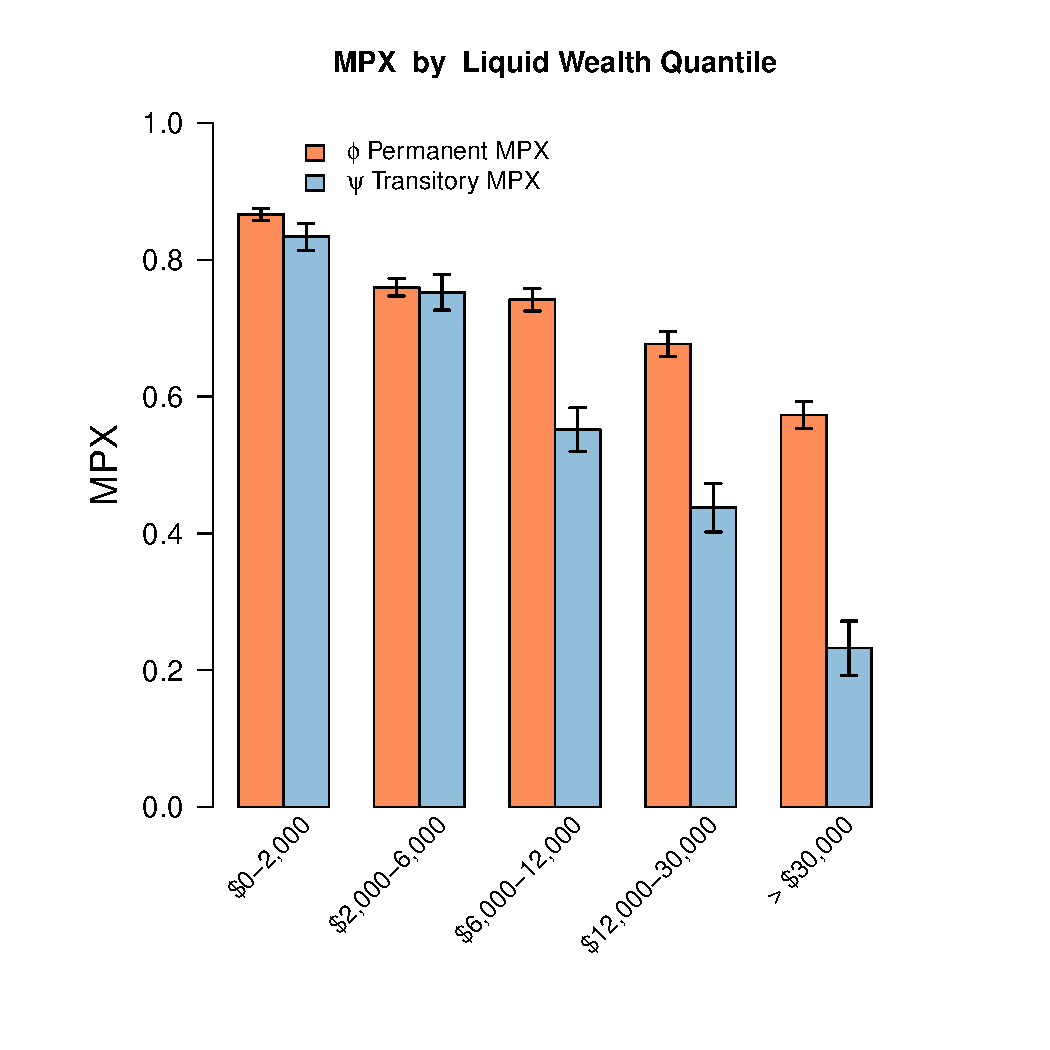
\includegraphics[scale=0.35]{../Figures/MPXByLiquidWealth_level_lincome_head.pdf}
	\column{0.5\linewidth}
	Key features:
	\begin{itemize}
		\item High overall Transitory MPC
		\item Decreasing with liquid wealth
	\end{itemize}
\end{columns}
}
\frame{
	\frametitle{Benchmark Model}
	Households maximize expected utility
	\begin{align*}
	\mathbb{E}_t \sum_{i=t}^{\infty} \beta^i u(\cLevBF_i)
	\end{align*}
	with:
	\begin{itemize}
		\item Permanent and Transitory shocks to income (calibrated to Danish data)
		\item Saving in one (liquid) asset
		\item No borrowing
		\item CRRA utility, $\rho = 2$
	\end{itemize}
}
\frame{
	\frametitle{Benchmark Model: Fitting the Liquid Wealth Distribution}
	Ex-ante heterogeneity in the discount rate\\
	\bigskip
	$\beta^i \sim \text{Unif}[ \beta_{\text{low}}, \beta_{\text{high}} ]$ Chosen to fit level and distribution of liquid wealth (especially at the low end)\\
	\centering
	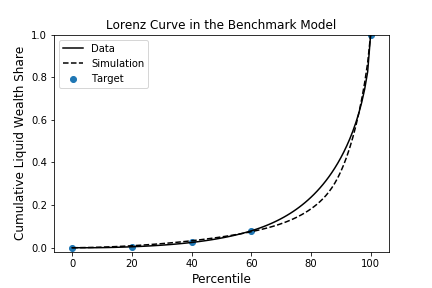
\includegraphics[scale=0.45]{../Figures/benchmark_Lorenz.png}	
}
\frame{
	\frametitle{Benchmark Model: Results}
	Simulate panel of data and estimate $\phi$ and $\psi$
	\begin{columns}
	\column{0.5\linewidth}
	\centering
	\begin{tikzpicture}
	\node (img1) {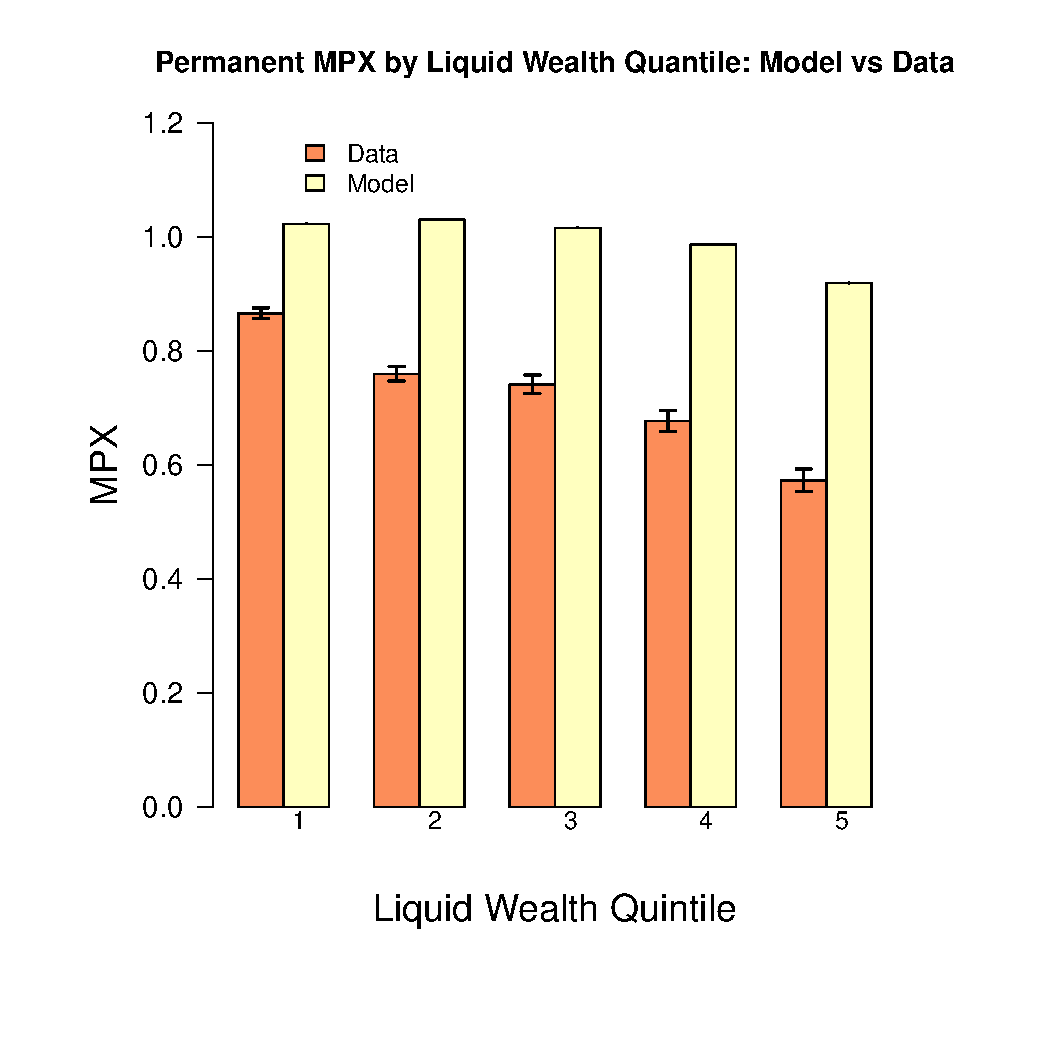
\includegraphics[scale=0.35]{../Figures/CSTW_perm_denmark.pdf}};
	\end{tikzpicture}
	\column{0.5\linewidth}
	\centering
	\begin{tikzpicture}
	\node (img3) {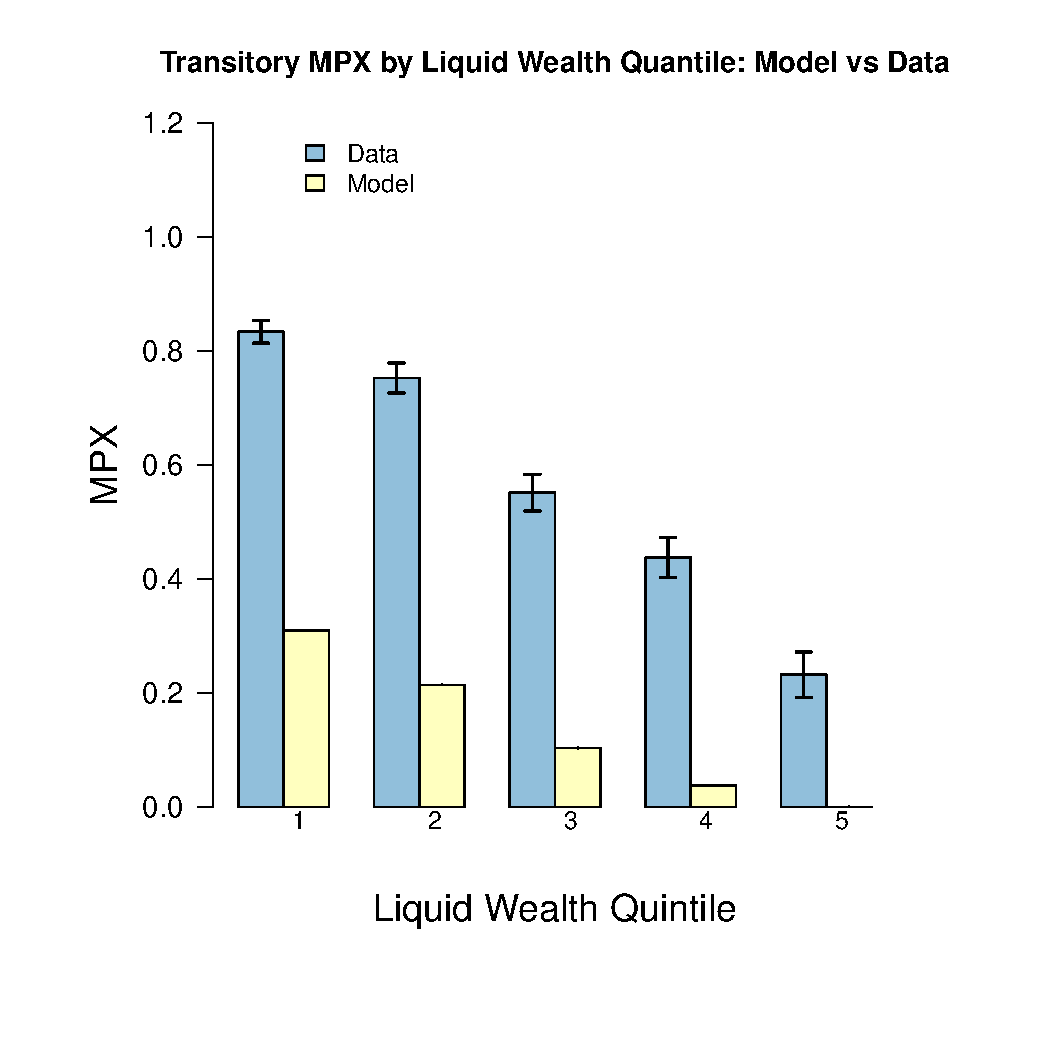
\includegraphics[scale=0.35]{../Figures/CSTW_tran_denmark.pdf}};
	\end{tikzpicture}
\end{columns} 	
}
\section{Model}
\frame{
	\frametitle{Taste Shock Model}
	\label{Model}
	First order problem: Transitory MPCs are too low\\
	\bigskip
	Need to lower $\beta$'s without reducing savings\\
	\bigskip
	Is income risk the only source of precautionary saving?
	\begin{itemize}
		\item In the data, expenditure FAR for volatile than income
		\item Surprise expenses can be large
	\end{itemize}
	Simple extension - add large taste shocks
	\begin{align*}
	\mathbb{E}_t \sum_{i=t}^{\infty} \beta^i \mathcal{X}_i u(\cLevBF_i)
	\end{align*}
}
\frame
{
	\frametitle{Taste Shock Model: Results}
	\begin{columns}
	\column{0.5\linewidth}
	\centering
	\begin{tikzpicture}
	\node (img1) {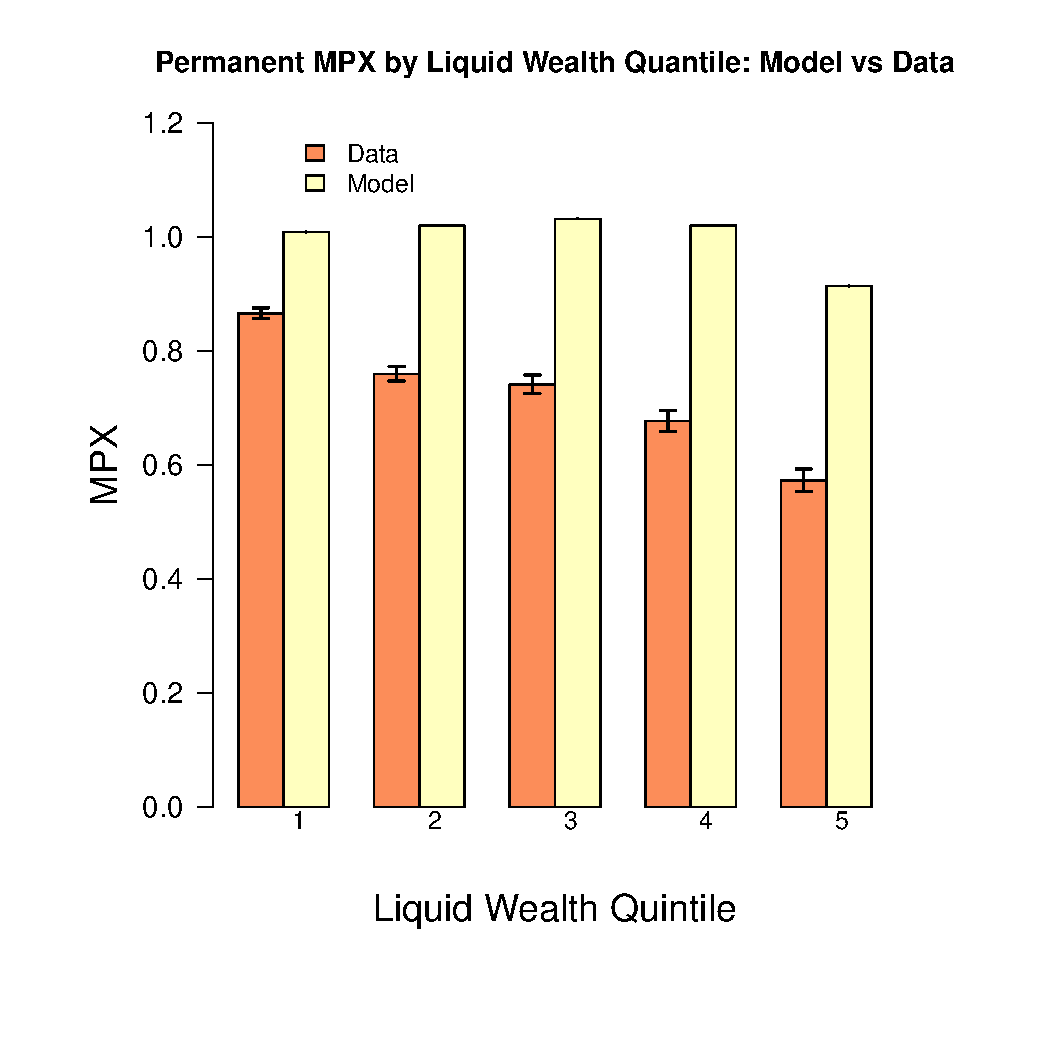
\includegraphics[scale=0.35]{../Figures/CSTW_perm_denmark_pref.pdf}};
	\end{tikzpicture}
	\column{0.5\linewidth}
	\centering
	\begin{tikzpicture}
	\node (img3) {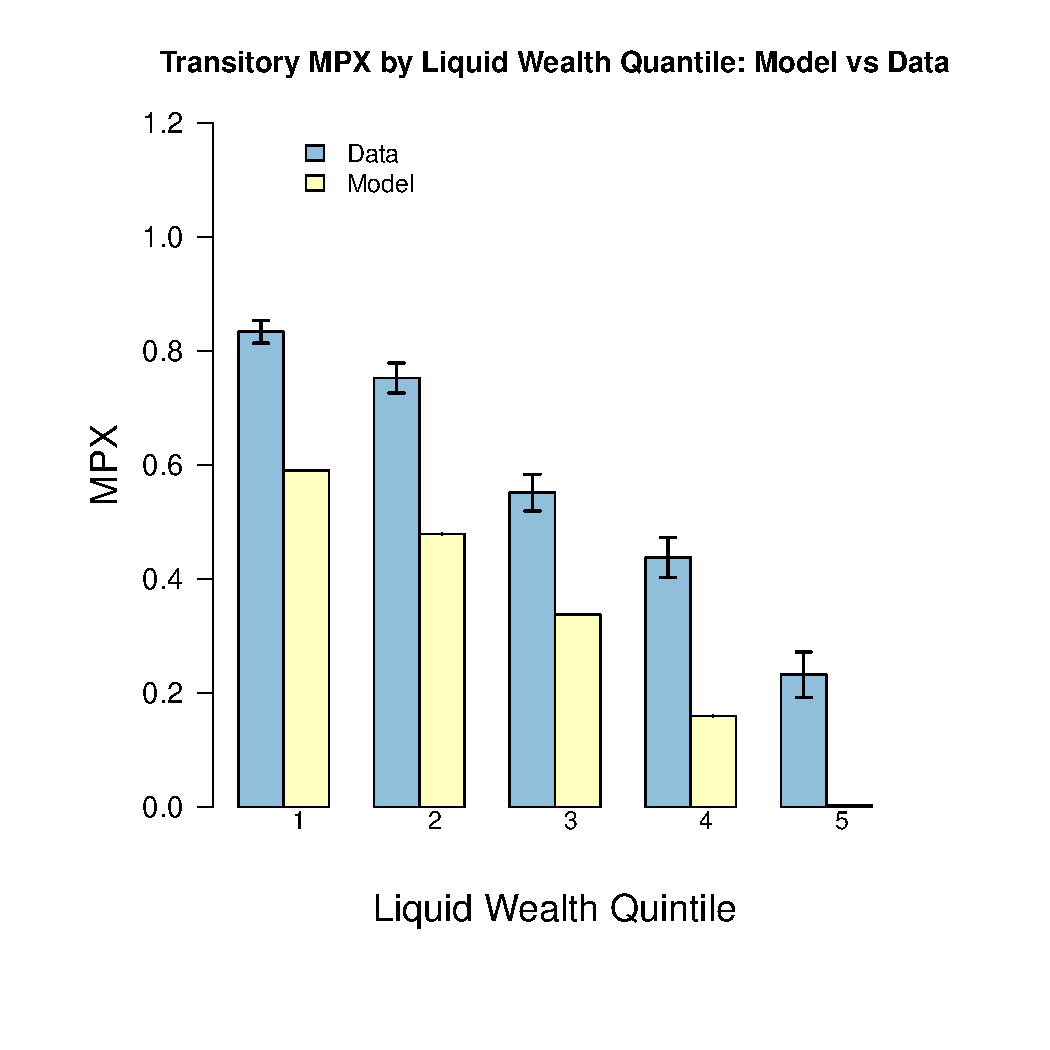
\includegraphics[scale=0.35]{../Figures/CSTW_tran_denmark_pref.pdf}};
	\end{tikzpicture}
\end{columns} 
}

\section{Threats to Identification}
\frame
{
	\frametitle{Endogenous Income Shocks}
	\begin{itemize}
		\item Household's consumption preference highly variable
		\item Hours worked is endogenous
	\end{itemize}
	The household maximizes:
	\begin{align*}
	\mathbb{E}_t \sum_{n=t}^{\infty} \beta^n \Bigg(\mathcal{X}_n \frac{ \cLevBF_n^{1-\rho}}{1-\rho}-\frac{\lLevBF_n^{1+\frac{1}{\xi}}}{1+\frac{1}{\xi}} \Bigg)
	\end{align*}
	\begin{itemize}
	\item Frisch elasticity $\xi$ 
	\item Preference shock $\mathcal{X}$
	\end{itemize}
}
\frame
{
	\frametitle{Endogenous Income Shocks}
	\input ../Tables/experimental/mpc_laborsupply.tex \\
	\input ../Tables/experimental/psi_laborsupply.tex
}
\frame
{
	\frametitle{Persistent Consumption Response}
	We assume the transitory consumption response lasts less than 2 years \\
	\begin{columns}
	\column{0.5\linewidth}
	\centering 
		High MPC Model\\
	\input ../Tables/experimental/Psi_array1.tex 
	\column{0.5\linewidth}
	\centering
	Low MPC Model\\
	\input ../Tables/experimental/Psi_array2.tex
\end{columns} 
	When MPCs are low, this assumption does not hold in the model, leading to downward bias		
}
\frame
{
	\frametitle{Income Measurement Error}
	Imputation method means measurement error in income shows up in consumption too\\
	Example:
	\begin{itemize}
		\item Actual transitory MPX is zero
		\item 25\% of transitory income variance is due to measurement error
		\item Methodology would result in MPX estimate of 25\%
	\end{itemize}	
	\pause
	But:
	\begin{itemize}
	\item Income is well measured (administrative data)
	\item Bias is much larger for households with small MPCs
	\begin{itemize}
		\item MPX for high liquid wealth households is close to zero
	\end{itemize}
\end{itemize}
}
\frame
{
	\frametitle{Permanent Shocks are AR(1)}
	How does our methodology do if permanent income follows an AR(1) process?
	\begin{align*}
	p_{t} = \rho p_{t-1} + \varepsilon_{t} \\
	y_t = p_t + q_t \\
	c_{t} = \phi y_t + \psi q_t
	\end{align*}
	\centering	
	\input ../Tables/experimental/psi_AR1.tex
}


%%%%%%%%%%%%%%%  bibliography
%%%%%%%%%%%%%%%%%%%%%%%%%%%%%%%%%%%%%%%%%%%%%%%%%%%%%%%%%%%%%%%%%%%%%%%%%%%%%%%%%%%%%%%%%%%%%%%%%%%%%%%%%%%%%%
\tiny

\beamerdefaultoverlayspecification{<*>}
\section{}

\begin{frame}[t,allowframebreaks]
	\frametitle{References}
	
	
	\bibliographystyle{\econtexBibStyle}
	\bibliography{Paper/AllPapers}
\end{frame}

\normalsize
\end{comment}
\bibliographystyle{\econtexBibStyle}
\newsavebox\mytempbib
\savebox\mytempbib{\parbox{\textwidth}{\bibliography{Paper/AllPapers}}}


\end{document}


